\documentclass[10pt,a4paper]{report} 

\usepackage[utf8]{inputenc}
\usepackage{amsmath}
\usepackage{amsfonts}
\usepackage{amssymb}
\usepackage{graphicx}
\usepackage[final]{pdfpages}
\usepackage{stmaryrd}
\usepackage{listings}
\usepackage[hidelinks]{hyperref}
\usepackage[english]{babel}
\usepackage{color}
\usepackage{fancyhdr}
\usepackage{xcolor}
\usepackage{url}
\usepackage{sectsty}
\usepackage{etoolbox}
\usepackage{tikz}
\usepackage[acronym]{glossaries}

% Abstract
\patchcmd{\abstract}{\null\vfil}{}{}{}

% Graphics and images
\graphicspath{{./images/}}

% Set headers to sans serif
\allsectionsfont{\sffamily}

% Defining colors for syntax highlighting
\definecolor{commentsColor}{rgb}{0.497495, 0.497587, 0.497464}
\definecolor{keywordsColor}{rgb}{0.000000, 0.000000, 0.635294}
\definecolor{stringColor}{rgb}{0.558215, 0.000000, 0.135316}

\lstset{aboveskip=20pt,belowskip=20pt}

% Source: https://denbeke.be/blog/programming/syntax-highlighting-in-latex/
\lstset{
  backgroundcolor=\color{white},
  basicstyle=\ttfamily\small,
  breakatwhitespace=false,
  breaklines=true,
  captionpos=b,
  commentstyle=\color{commentsColor}\textit,
  deletekeywords={...},
  escapeinside={\%*}{*)},
  extendedchars=true,
  frame=tb,
  keepspaces=true,
  keywordstyle=\color{keywordsColor}\bfseries,
  %language=Python,
  otherkeywords={*,...},
  %numbers=left,
  numbersep=5pt,
  numberstyle=\tiny\color{commentsColor}, 
  rulecolor=\color{black}, 
  showspaces=false,
  showstringspaces=false,
  showtabs=false, 
  stepnumber=1, 
  stringstyle=\color{stringColor},
  tabsize=2, 
  title=\lstname,
  columns=fixed 
}

% Bibliography
\bibliographystyle{unsrturl}

% Pagestyle
\pagestyle{fancy}

% Hyperlinks
\hypersetup{
  colorlinks=true,
  allcolors=black
}


\begin{document}

\title{
\vspace{-80px}
\includegraphics[width=5cm]{bfh-logo}\\
\vspace{80px}
\huge\textsf{\textbf{3D Terrain with Level of Detail}}\\
\vspace{50px}
\large{Written report for the module\\
BTI3041 -- Project 2\\ 
by\\}
\vspace{20px}
\Large{Amar Tabakovic\\}
\vspace{40px}
\large{
\textbf{Bern University of Applied Sciences}\\
  Engineering and Information Technology\\
  Computer Perception \& Virtual Reality Lab
\\
\vspace{20px}
\textbf{Supervisor}\\
Prof. Marcus Hudritsch}\\
\vspace{30px}
\today
}

\date{}
\maketitle

\begin{abstract}
 Rendering terrains is a central task for video games, geographic information systems and simulation software, 
 but also computationally expensive. Optimizations, one of which is the level of detail (LOD),
 are necessary in order to ensure adequate performances.
 Numerous algorithms were developed in the last 30 years which tackle the problem of efficient terrain rendering.
 A demo terrain renderer is developed with the goal to demonstrate and compare some of the ideas of these algorithms.
 The main implemented algorithm is mostly based on GeoMipMapping \cite{geomipmapping}, but also draws inspiration from GPU-based Geometry Clipmaps \cite{gpugeomclipmaps}
 and other approaches.
 The implementation was tested on a $14000 \times 14000$ heightmap of Switzerland and bordering regions, yielding around 
 60 FPS on a 2020 MacBook Air while delivering decent visualizations.
\end{abstract}

\tableofcontents

\listoftables
\listoffigures
\lstlistoflistings

\chapter{Introduction}
In the field of 3D computer graphics, rendering is one of the central tasks.
Many practical applications of 3D computer graphics make use of terrains, 
such as flight simulators, open-world video games, and Geographic Information Systems (GIS) \cite[p.~185]{lodfor3dgraphics}.
At the same time, rendering large and constantly visible objects, such as the terrain, is computationally expensive 
and optimizations are necessary in order to avoid performance deficiencies.

One area which offers potential for optimizations is the \textit{level of detail (LOD)} of objects.
The concept of LOD is based on the idea that the farther away an object is, the fewer details are going to be visible to the human eye.

The problem of rendering terrains spawned numerous algorithms and approaches specifically
for this purpose. 

\section{Goals of this Project}
%The goals of this project can be formulated as follows:
The main goal of this project is to gain an overview over the field of 
terrain LOD. This includes analyzing and comparing a selection of terrain LOD algorithms and approaches,
including implementing as part of a demo computer application.

% \begin{itemize}
%   \item Introduction to terrain LOD: 
% \end{itemize}
% Goals: Introduction to LOD and terrain LOD, give overview of algorithms and implementations, 
%        overview of applications in game engines and other, demo application for trying out LOD algorithms, 
%        performance comparison 

\section{Structure of the Report}
This report is structured as follows:
\begin{itemize}
  \item 
\end{itemize}



\chapter{Basics of Terrain Rendering}
\section{Terrain Data Representation}
\subsection{Heightmaps}
One way of representing terrains is using \textit{heightmaps}.
A heightmap is a $n\times n$-grid that contains 
the height value $y$ for each $(x,z)$-position\footnote{We always denote $y$ for the up direction except if explicitly stated otherwise.}.
Positions are always spaced evenly in a grid-like manner,
but the distance between any two neighboring positions is variable.

The main advantage of heightmaps is that they allow for very simple storage and manipulation of height data, e.g. in form of images,
where low color values represent low areas of terrain and vice versa for
high color values. For a grayscale image, up to 256 height values can be used and for an RGB image,
more than 16 million height values are supported.
Looking up a height value for a given $(x,z)$-position is easy as well,
which consists of a simple lookup at the given position in the image.
Figure~\ref{fig:dom} shows a $2000 \times 2000$ heightmap of the mountain Dom in Valais, Switzerland.
\begin{figure}[H]
  \centering
  \includegraphics[width=0.4\textwidth]{dom}
  \caption{$2000 \times 2000$ heightmap of the mountain Dom in Valais, Switzerland retrieved from SwissTopo \cite{alti3d}.}\label{fig:dom}
\end{figure}

\subsection{Triangulated Irregular Networks}
An alternative to the heightmap is the \textit{triangulated irregular network (TIN)} data structure.
A TIN consists of a collection of 3D vertices, where 
the arrangement of vertices can be irregular. Figure~\ref{fig:tin-example} shows 
an example of a TIN.
\begin{figure}[H]
  \centering
  \includegraphics[width=0.52\textwidth]{tin-example}
  \caption{Example of a TIN. Note that the left area represents a terrain area with many changes 
  (e.g. mountains, hills, etc.), and the right area represents an area with few changes (e.g. flat areas).}\label{fig:tin-example}
\end{figure}

The main advantage of TINs is that fewer polygons need to be used for 
e.g. smooth terrain areas. Another advantage is that
special terrain features can be modelled 
which are usually difficult to model with heightmaps, such as overhangs, cliffs and caves, 
The disadvantage of TINs, however, is that the full $(x,y,z)$ coordinates need to be stored,
whereas with heightmaps, only the height value $y$ needs to be stored.

\section{Bintrees and Quadtrees}
\textit{Binary triangle trees (bintrees)} and \textit{quadtrees} are 
recursive data structures based on triangles and quads respectively.
A bintree consists of up to two child triangles, both of which in turn also consist of up to two child triangles each, and so on.
Quadtrees are structured similarly, with a quad consisting of up to four child quads, and each child quad consisting
of up to four child quads, and so on.
Figure~\ref{fig:bintree-quadtree-example} shows an example of a bintree and a quadtree.

\begin{figure}[H]
  \centering
  \subfloat[\centering]{{\includegraphics[width=0.43\textwidth]{bintree-example} }}
  \qquad
  \subfloat[\centering]{{\includegraphics[width=0.33\textwidth]{quadtree-example.png} }}%
  \caption{Example of a bintree (a) and a quadtree (b).}\label{fig:bintree-quadtree-example}
\end{figure}

The main advantage of bintrees and quadtrees is that 
LOD can be modelled very naturally with them.
Bintree/quadtree sections with few children correspond to a low LOD and 
vice versa for bintree/quadtree sections with many children.

\section{Potential Problems During Terrain Rendering}
While terrain LOD algorithms dramatically improve the performance of terrain rendering, 
there are certain faults that can occur during rendering. 

\subsection{Cracks}
Cracks and holes in terrains can appear when a higher LOD terrain section is bordered 
by a lower LOD terrain section. The main problem is that when a vertex $v_{\text{high}}$ of a higher LOD terrain section lies on the edge $e_{\text{low}}$
of a lower LOD terrain section and the $y$ coordinate of $v_{\text{high}}$ is greater or less than the 
height of $e_{\text{low}}$ at that point, the difference in height causes the crack to appear, as shown in figure~\ref{fig:crack-example}.
\begin{figure}[H]
  \centering
  \subfloat[\centering The crack is caused by the height difference of $v_{\text{high}}$ and $e_{\text{low}}$.]{{\includegraphics[width=0.5\textwidth]{crack-example} }}
  \qquad
  \subfloat[\centering The background color is set to red to highlight the cracks.]{{\includegraphics[width=0.4\textwidth]{cracks-terrain} }}%
  \caption{Illustration of a crack (a) and some examples of cracks in a real rendered terrain (b).}\label{fig:crack-example}
\end{figure}
Cracks can be solved by either of the following, depending on the capabilities of the LOD approach:
\begin{itemize}
  \item Removing the vertex in question, cuasing the higher and lower LOD meshes to be connected seamlessl (in figure~\ref{fig:crack-example} vertex $v_{\text{high}}$).
  \item Inserting an extra vertex at the border edge of the lower LOD mesh \cite[p.~194]{lodfor3dgraphics} (in figure~\ref{fig:crack-example} on top of vertex $v_{\text{high}}$). The disadvantage of this is that an extra vertex needs to get created.
  \item By force splitting the terrain mesh to get a more continuous mesh \cite[p.~193]{lodfor3dgraphics}. 
\end{itemize}

\subsection{Popping}
The phenomenon of \textit{popping} occurs when the camera is moving 
and the transition of the terrain's LOD level causes visual pops to appear.
Popping decreases the realism of the terrain and should be as minimal as possible.
Popping can be reduced by introducing \textit{vertex morphing} \cite{geomipmapping,geomclipmaps,cdlod}, 
i.e. by animating the transition of one LOD level to the next seamlessly through interpolation.
\chapter{Existing Work and Literature}
This chapter starts off by presenting some of the existing algorithms and approaches to terrain rendering.
Afterwards, a selection of real-world systems are given, in which terrain LOD algorithms are used.

\section{Algorithms and Approaches for Terrain LOD}
Terrain LOD is a well-researched topic and over the last three decades, numerous approaches have been published.
In the following, some of the most important publications are listed in chronological order.
The approaches that are described in greater detail in the upcoming subsections are highlighted in \textbf{bold}:
\begin{itemize}
  \item ``Real-Time, Continuous Level of Detail Rendering of Height Fields'' \cite{lindstrom1996} by Lindstrom \textit{et al.} in 1996.
  \item \textbf{``ROAMing Terrain: Real-time Optimally Adapting Meshes''} \cite{roam} by Duchaineau \textit{et al.} in 1997.
  \item ``Real-Time Generation of Continuous Levels of Detail for Height Fields'' \cite{rottgerpaper} by Röttger \textit{et al.} in 1998.
  \item \textbf{``Fast Terrain Rendering Using Geometrical MipMapping''}  \cite{geomipmapping} by de Boer in 2000.
  \item ``Rendering Massive Terrains using Chunked Level of Detail Control'' \cite{chunkedlod} by Ulrich in 2002.
  \item ``Geometry Clipmaps: Terrain Rendering Using Nested Regular Grids'' \cite{geomclipmaps} by Hoppe and Losasso in 2004 and the follow-up \textbf{``Terrain Rendering Using GPU-Based Geometry Clipmaps''} by Asirvatham and Hoppe \cite{gpugeomclipmaps} in 2005.
  \item ``Continuous Distance-Dependent Level of Detail for Rendering Heightmaps (CDLOD)'' \cite{cdlod} by Strugar in 2009.
  \item \textbf{``Concurrent Binary Trees (with application to longest edge bisection)''} \cite{cbt} by Dupuy in 2020.
\end{itemize}
In the following subsections on the algorithms, all presented ideas are taken from their respective original publications,
unless noted otherwise.

\subsection{ROAM}
\textit{ROAM} (short for \textbf{R}eal-time \textbf{O}ptimally \textbf{A}dapting \textbf{M}eshes) 
is a terrain LOD algorithm developed by Duchaineau \textit{et al.} \cite{roam} published in 1997.
ROAM represents the terrain mesh using bintrees and performs triangle splits and merges
for generating and removing detail.

The central idea of the algorithm is to use temporal coherence: often, between two frames 
the meshes are very similar. This means that the mesh from a previous frame can be used to compute 
the mesh of the current frame, rather than building up the mesh from ground up.
This is done using two priority queues: a split queue $\mathcal{Q}_s$ and a merge queue $\mathcal{Q}_m$.
The split queue contains splittable triangles $T$
and the merge queue contains mergable triangle pairs $(T,T_B)$.
At each frame, the terrain mesh gets split and merged using $\mathcal{Q}_s$ and $\mathcal{Q}_m$. until either the required size/accuracy is reached
or the time runs out. 
The splits and merges always result in a continuous mesh, i.e. the mesh cannot contain any 
T-junctions.
The elements of $\mathcal{Q}_s$ and $\mathcal{Q}_m$ are ordered by 
various geometric error metrics, some of which are the following:
\begin{itemize}
  \item Nested bounding volumes named \textit{wedgies}, which are defined to include the entire $x$ and $z$ extent of a triangle and its subtriangles 
        plus some padding space above and below the highest and lowest points respectively. Wedgies are computed while building the initial mesh at the beginning of the algorithm.
  \item Another metric is the distance between where a node is supposed to be on the screen and where the algorithm actually placed the node.
        The maximum of all distances is calculated and used as the base priority metric of the algorithm.
\end{itemize}

While the bintree trees gets traversed, various flags are updated which indicate whether a wedgie is inside the view-frustum, partially or not at all.
ROAM is designed as a greedy algorithm, meaning it will always performs the most optimal splits/merges for each frame.


\subsection{GeoMipMapping}
\textit{Geometrical Mipmapping (GeoMipMapping)} is a terrain LOD approach published by de Boer \cite{geomipmapping} in the year 2000.
The central idea of GeoMipMapping is its analogy to texture mipmapping: just like how textures of far away objects are rendered using lower resolution texture mipmaps,
terrain areas that are far away from the camera should also be rendered with a lower resolution mesh.

This is achieved by splitting up the terrain into so-called \textit{blocks} (also called \textit{patches}) of a fixed side length $2^n + 1$ for some $n \in \mathbb{N}$.
Each block has a LOD level\footnote{The original GeoMipMapping paper uses 0 to denote the maximum LOD level and vice-versa for the minimum LOD level. In order to avoid any confusion with the term \textit{LOD}, this report denotes 0 as the minimum LOD level and vice versa for the maximum LOD level.} $0\leq l \leq n$ that changes dynamically at runtime.
Each representation of a block at a specific LOD level is called a \textit{GeoMipMap}.
For each GeoMipMap, the number of vertices on one side is $2^{l}+1$ and the number of quads is $2^{2l}$.
Figure~\ref{fig:geomipmapping-patch-example} shows an example of a $5 \times 5$ block at LOD levels 2, 1 and 0.

\begin{figure}[H]
  \centering
  \subfloat[\centering LOD level 2 (maximum).]{{\includegraphics[width=0.28\textwidth]{geomipmapping-level-2.png} }}
  \qquad
  \subfloat[\centering LOD level 1.]{{\includegraphics[width=0.28\textwidth]{geomipmapping-level-1.png} }}
  \qquad
  \subfloat[\centering LOD level 0 (minimum).]{{\includegraphics[width=0.28\textwidth]{geomipmapping-level-0.png} }}
  \caption{Example of each GeoMipMap of a $5 \times 5$ block. The omitted vertices of lower LOD GeoMipMaps are marked as dotted circles (based on \cite{geomipmapping}).}\label{fig:geomipmapping-patch-example}
\end{figure}

The organisation of the terrain into blocks allows for easy view-frustum culling, which is performed 
with a quadtree, where each node contains the AABB of its four children and the leaf nodes 
contain the actual blocks.

The LOD level for each block is selected at runtime and is based on the 
screen-space error that is caused by changing the LOD level of a block.
When the LOD level of a block changes, vertices get added or removed from the block,
which causes a difference in height $\delta$ between the two GeoMipMaps of that block. Projecting $\delta$ into 
screen-space yields $\varepsilon$. 
This $\varepsilon$ can be limited with a threshold $\tau$, such that 
the change in LOD level occurs only if $\varepsilon < \tau$.
The LOD selection can be sped up by pre-computing $\varepsilon$ per GeoMipMap and storing it in a look-up table.

GeoMipMapping avoids cracks by checking the four neighboring blocks
of a block and omitting the vertices that would cause cracks in the terrain.
The vertex omission is performed by rendering the bordering row/column of the current block
as triangle fans, as shown in figure~\ref{fig:geomipmapping-crack-avoidance}.

\begin{figure}[H]
  \centering
  \includegraphics[width=0.7\textwidth]{geomipmapping-crack-avoidance}
  \caption{Example of GeoMipMapping's crack avoidance between a LOD 2 and a LOD 1 GeoMipMap of two $5 \times 5$ blocks (based on \cite{geomipmapping}).}\label{fig:geomipmapping-crack-avoidance}
\end{figure}

Some further optimizations that were mentioned, which extend the just described basic GeoMipMapping algorithm, 
are \textit{trilinear GeoMipMapping} (i.e. morphing the vertices at LOD transitions similarly to trilinear mipmapping),
and \textit{progressive GeoMipMap streaming}.

\subsection{(GPU-based) Geometry Clipmaps}
Geometry Clipmaps \cite{geomclipmaps} is a terrain rendering technique published by Hoppe and Losasso in 2004.
A follow-up GPU-based variant of Geometry Clipmaps \cite{gpugeomclipmaps} was published in GPU Gems 2 by Hoppe and Asirvatham in 2005.
In this section, the basic features of the GPU-based Geometry Clipmaps algorithm are described,
and we leave out some more advanced features, such as compression and noise-generated details.

The algorithm is based on a single flat mesh centered around the camera.
The flat mesh is organized as a set of nested rings of $l$ levels, 
where the innermost level $l-1$ is a filled-in $n \times n$ grid, and where the ring at level $i$ is twice as big as the ring 
at level $i + 1$. This $n$ must be of the form $2^k - 1$ for some $k \in \mathbb{N}$. 
Each ring at a level is organized into 12 blocks of size $m \times m$, where $m = (n+1)/4$.
Gaps inbetween the blocks are filled up with special types of blocks, namely the $m \times 3$ \textit{ring fix-up} and the $(2m+1) \times n$ \textit{interior trim}.
In order to avoid T-junctions, a string of degenerate triangles is rendered at the border between blocks of 
different size. Since each block is identical up to translation and uniform scale, they get stored once on a vertex and index buffer 
and translated and scaled in the vertex shader at runtime, which greatly reduces memory consumption.
Figure \ref{fig:geometry-clipmaps-mesh} shows an example of this mesh. 

\begin{figure}[H]
  \centering
  \includegraphics[width=1.0\textwidth]{geometry-clipmaps-mesh}
  \caption{Example of the flat mesh in Geometry Clipmaps with $n = 15$, $m = 4$ and $l = 3$ (based on \cite{gpugeomclipmaps}).}\label{fig:geometry-clipmaps-mesh}
\end{figure}

In the vertex shader, the algorithm samples the height values from the heightmap texture.
Additionally, it performs the calculations for the so-called \textit{transition regions}, 
which are regions near the border of two levels in which 
the levels get morphed, so that the transition between levels is smooth and no popping occurs.
The morphing is performed by computing the blend factor $\alpha$,
which is based on the position of the viewer and the position of the vertex in world-space.
This factor $\alpha$ is defined such that it is 0 everywhere except at the transition region,
which then linearly grows to 1 until reaching the border.

During rendering, view-frustum culling is performed by intersecting each block with the view-frustum,
and if the AABB of the block does not intersect the view-frustum, it does not get rendered.

Shading is performed with a normal map, which has twice the resolution of the heightmap.
The normal map is computed whenever the clipmap gets updated.

\subsection{Concurrent Binary Trees}
The \textit{concurrent binary tree (CBT)} is a data structure published by Dupuy in 2020.
It essentially allows for binary trees to be computed in parallel using a binary heap 
stored as a bitfield. This allows for easy concurrent manipulation of tree nodes using bitwise operations.
The data structure is applicable to problems relying on binary trees, 
such as the \textit{longest edge bisection}.

The paper contains a section describing the application of CBTs to terrain rendering.
The approach is similar to \cite{roam} in the sense that it computes a triangulation of the terrain using bintree splitting and merging.
The main difference is that the spliting and merging of the bintrees happens in parallel on compute shaders with the 
CBT data structure, whereas in \cite{roam}, the bintrees are split and merged on the CPU.
The split and merge criteria are defined such that sub-pixel rasterization is avoided.
Triangles outside of the view-frustum and triangles at flat areas are not split or merged further.

Dupuy claims

An issue which is not adressed in the paper is how popping is avoided in the terrain.

\subsection{Conclusion}
In this subsection, the algorithms and their suitability for implementation are discussed.

\paragraph{ROAM} ROAM is not particularly suited for today's GPU, since it mainly relies 
on immediate mode rendering \cite{geomclipmaps}, which is outdated in most graphics APIs of today.
In addition to this, the costly splits and merges of the priority queues happen entirely on the CPU,
which is undesirable.

\paragraph{GeoMipMapping} The strongest point of GeoMipMapping is the fact that its easy to understand and 
to implement.
GeoMipMapping was published at a time in which immediate mode was widely-used.
Nowadays, mmediate mode is deprecated in most graphics APIs.
In order for GeoMipMapping to be suitable for modern GPUs, it needs to be modified such that 
it can work with vertex and index buffers, which is feasible thanks to its block-based nature.

\paragraph{Geometry Clipmaps} GPU-based Geometry Clipmaps was one of the first algorithms to utilize 
the vertex texturing functionality of GPU, which was newly introduced at the time of its publication.
The fact that only very few vertices and indices are required (which are translated and scaled during rendering to their corresponding position) 
and the fact that the heightmap can be sampled in the vertex shader makes GPU-based Geometry Clipmaps still a suitable 
approach for modern hardware. This is reflected in the fact that the most widely-used Godot plugin for heightmap rendering 
is based on GPU-based Geometry Clipmaps, (see the next section).
Some other strong points are the transition regions for avoiding pops, its configurability, and the fact that 
no LOD determination has to be performed, since the mesh is constant.

\paragraph{CBT} The CBT data structure ``revitalized'' mesh-subdivision-based approaches, such as \cite{lindstrom1996,roam},
since bintrees can now be computed in parallel with compute shaders, rather than on the CPU. However, some aspects are not yet handled, such as 
preventing pops. It is a rather new approach that has not yet been tested in the real-world.

\paragraph{Overall Conclusion}
Overall, algorithms which load the vertices and indices once to the GPU and do not touch the buffers again 


\section{Terrain LOD in Real-world Systems}
\subsection{Game Engines}
\subsubsection{Godot}
Godot is a cross-platform game engine written in C\#, C++ and its own scripting language GDScript.
Terrains are supported in form of extensions developed by community members, 
which can be installed and used in Godot projects by game developers.

One such extension is Terrain3D by Cory Petkovsek \cite{godotterrain3dgithub} 
written in C++ for Godot 4. The LOD approach used in this extension is based on 
geometry clipmaps by Hoppe and Losasso \cite{geomclipmaps}. % TODO Explain algo in high-level fashion
The concrete implementation
of the geometry clipmap mesh code was created by Mike J Savage \cite{geomclipmapssavage}. 

% TODO https://github.com/Zylann/godot_heightmap_plugin/blob/11e0db92c2f8e0e907ae173b983d73af1e35c4c2/addons/zylann.hterrain/doc/docs/index.md
Another extension for terrains is Godot Heightmap Plugin by Marc Gilleron \cite{godotheightmapplugingithub} written in GDScript and C++.
The extension uses a quadtree-based approach for terrain LOD. 

\subsubsection{Unity}
Unity is another cross-platform game engine written in C\# and C++, and has a 
built-in terrain system. 
The core engine source code of Unity is only accessible
by owning an enterprise licence, therefore no information is given on which 
specific terrain LOD algorithm is used for the built-in terrain in Unity.
Instead, a high-level overview of Unity's terrain system is given 
and some additional information on related projects.

The terrain system supports importing and exporting of heightmaps in 
the RAW file format, with either an 8-bit or 16-bit grayscale value per pixel.
Visually, the mesh of the terrain LOD resembles that from a quadtree-based LOD approach, such as \cite{chunkedlod}.
The Unity terrain does not perform any morphing between different LOD levels,
which means that pops are visible at LOD level changes.

There exists an open-source library for hierarchical LOD in Unity called HLODSystem developed by JangKyu Seo at Unity TODO citation .
HLODSystem also supports terrains with its TerrainHLOD component, allowing for conversion from an Unity Terrain object to a HLOD mesh with configurable parameters, such as chunk size and border vertex count.
HLODSystem allows the developer to specify the mesh simplifier to be used and currently the only supported simplifier is UnityMeshSimplifier, 
an open-source mesh simplifier developed by TODO that utilizes the fast quadratic mesh simplification algorithm developed by Sven Forstmann TODO citation.

The previously described CBT data structure and its application to terrain rendering was published by Dupuy 
at Unity Labs. 
At SIGGRAPH Courses 2021, Deliot et al. gave a talk in which they described some additional implementation details 
and the (potential) integration into the Unity game engine. As of today, Unity does not yet use 
the CBTs for its terrain system.

\subsubsection{Unreal Engine}
Unreal Engine is another cross-platform game engine written in C++ and features
an integrated terrain system called the Landscape system.

The maximum supported heightmap size is $8192 \times 8192$.


\subsubsection{Frostbite}
Frostbite is a closed-source game engine developed by DICE and is known for the \textit{Battlefield} series.
DICE has held numerous talks in the last few years describing iterations of their
terrain system.
During the Game Developers Conference 2012, DICE presented the terrain system of \textit{Battlefield 3}, which was developed with their Frostbite 2 engine.
They mention a quadtree-based terrain LOD system and describe several optimizations regarding paging and streaming of terrain.
TODO cite.

% \subsection{Geographic Information Systems}
% TODO: Check out Google maps, Google Earth, other GIS
% TODO: Maybe look at flight simulators (if information available)


% \section{Research Articles and Publications}
% Terrain LOD is a well-researched topic and over the last three decades, numerous approaches have been published.
% In the following, some of the most important publications are listed in chronological order.
% The approaches that are described in greater detail in chapter ``Algorithms and Approaches for Terrain LOD'' are highlighted in \textbf{bold}:
% \begin{itemize}
%   \item ``Real-Time, Continuous Level of Detail Rendering of Height Fields'' \cite{lindstrom1996} by Lindstrom \textit{et al.} in 1996.
%   \item \textbf{``ROAMing Terrain: Real-time Optimally Adapting Meshes''} \cite{roam} by Duchaineau \textit{et al.} in 1997.
%   \item ``Real-Time Generation of Continuous Levels of Detail for Height Fields'' \cite{rottgerpaper} by Röttger \textit{et al.} in 1998.
%   \item \textbf{``Fast Terrain Rendering Using Geometrical MipMapping''}  \cite{geomipmapping} by de Boer in 2000.
%   \item ``Rendering Massive Terrains using Chunked Level of Detail Control'' \cite{chunkedlod} by Ulrich in 2002.
%   \item ``Geometry Clipmaps: Terrain Rendering Using Nested Regular Grids'' \cite{geomclipmaps} by Hoppe and Losasso in 2004 and the follow-up \textbf{``Terrain Rendering Using GPU-Based Geometry Clipmaps''} by Asirvatham and Hoppe TODO Cite in 2005.
%   \item ``Continuous Distance-Dependent Level of Detail for Rendering Heightmaps (CDLOD)'' \cite{cdlod} by Strugar in 2009.
%   \item \textbf{``Concurrent Binary Trees (with application to longest edge bisection)''} TODO cite by Dupuy in 2020.
% \end{itemize}

% \section{Game Developers Conference}
% The \textit{Game Developers Conference} is a yearly conference for professionals in the game development industry.
% Numerous game development companies have held technical talks about their terrain systems.
% The slides, papers and video recordings of the talks are available online on GDC's homepage.
% % TODO

% \section{Level of Detail for Computer Graphics}
% \textit{Level of Detail for Computer Graphics} by Luebke \textit{et al.} \cite{lodfor3dgraphics} 
% is a reference book for the topic of 
% LOD published in 2002. The book builds on top of years of research in the 
% area of LOD and provides an overview to many LOD techniques. For this project,
% chapter 7 ``Terrain Level of Detail'' of the book is especially relevant, 
% as it dives into the topic of LOD for terrains specifically.
% It covers basic approaches and techniques for terrain LOD, 
% common problems that can arise during rendering of terrains and some solutions to them, 
% and a catalog of terrain LOD algorithms.

% \section{Focus on 3D Terrain Programing}
% \textit{Focus on 3D Terrain Programming} by Trent Polack \cite{focuson3dterrainprogramming} is a book about terrain programming published in 2002.
% Part one of the book introduces the reader to the basics of terrains, such as heightmaps and texturing. Part two then 
% covers some more advanced topics, including a selection of terrain LOD algorithms. The presented LOD algorithms are
% ROAM \cite{roam}, Röttger's quadtree-based algorithm \cite{rottgerpaper}, and GeoMipMapping \cite{geomipmapping}.
% The book also includes demo source code written in C++ and OpenGL, albeit somewhat outdated today.

% \section{Virtual Terrain Project}
% The \textit{Virtual Terrain Project} \cite{vtp} was a project run from 2001 to 2013 
% that consisted of a collection of software, information and resources on terrain modelling and rendering,
% including a large overview of publications and implementations related to terrain LOD algorithms.

\chapter{ATLOD: A Terrain Level of Detail (Renderer)}
This chapter describes \textit{ATLOD} (short for \textbf{A} \textbf{T}errain \textbf{L}evel \textbf{o}f \textbf{D}etail (Renderer)), the demo terrain rendering application.

\section{Preliminaries}
\subsection{Used Technologies}
ATLOD is written in C++17 and OpenGL 4.2.
For compiling build files, CMake (minimum version 3.5) is used.
ATLOD uses the following third-party libraries:
\begin{itemize}
  \item GLM: The \textit{OpenGL Mathematics (GLM)} library provides functionality for the mathematics of graphics programming, such as classes for vectors, matrices and perspective transformations.
  \item GLEW: The \textit{OpenGL Extension Wranger Library (GLEW)} is an extension loading library for OpenGL. 
  \item GLFW: \textit{GLFW} is a multi-platform library for desktop-based OpenGL applications, offering an API for managing windows, contexts and input handling.
  \item STB: STB is a collection of header-only libraries developed by Sean Barrett TODO cite. ATLOD uses \texttt{stb\_image.h} for loading images of heightmaps and textures.
\end{itemize}

The source code is hosted on GitHub on the repository AmarTabakovic/3d-terrain-with-lod
and is licensed under TODO.

\subsection{Chosen Algorithms}
The chosen algorithms and their reasons for implementing them are the following:
\paragraph{Naive Brute-force Algorithm} The naive brute-force algorithm consists of simply reading in all height values from the heightmap as vertices and rendering them directly to the screen.
The main reason for implementing the naive brute-force algorithm is to motivate the usage of terrain LOD algorithms by showing the difference in performance
compared to the optimized LOD approaches.

% TBD, depends on how far I come
\paragraph{GeoMipMapping} The main reason for implementing GeoMipMapping is to have at least one CPU-based approach
as a reference point for comparison with GPU-based approaches.
In addition, GeoMipMapping is considered to be relatively straightforward to implement \cite[p.~79]{focuson3dterrainprogramming}.

% \paragraph{Hoppe and Lossaso's Geometry Clipmaps} TODO
% \paragraph{Strugar's CDLOD} TODO

\section{Height and Texture Data}
\subsection{Data Sources}
\subsubsection{SwissTopo}

\subsubsection{SRTM}

\subsection{Supported Formats}
The following file formats are supported for loading heightmaps:
\begin{itemize}
  \item \texttt{.png} and \texttt{.jpg}: Heightmaps can be loaded as PNG and JPG images. This is implemented using \texttt{stb\_image.h}.
  \item \texttt{.asc}: Heightmaps as ASCII grids are supported. Digital elevation data from the Shuttle Radar Topography Mission (SRTM) is delivered in ASCII grid format.
  \item \texttt{.xyz}: the XYZ format is based on SwissTopo
\end{itemize}


\section{Basic Setup and Architecture}
\subsection{Overview}
TODO High-level class diagram
\subsection{Shaders}

\subsection{Camera}

\subsection{Heightmap}

\subsection{Terrain}
Each terrain LOD algorithm is encapsulated in a class, which inherits from the base terrain class \texttt{Terrain}.
The base terrain is structured as shown in listing TODO.

\section{Naive Brute-force Algorithm}
The naive brute-force algorithm, which simply renders every vertex without any LOD considerations, is encapsulated in the class \texttt{NaiveRenderer}.

The method \texttt{loadBuffers()} loads the height data from the heightmap directly into a vertex buffer with the ID \texttt{terrainVBO} and the indices into an index (i.e. element) buffer named \texttt{terrainEBO}.
The indices are organized such that they can be rendered as triangle strips with \texttt{GL\_TRIANGLE\_STRIPS}.
Each row is separated using a special marker index named \texttt{RESTART}, which is set to the maximum possible \texttt{GLuint} value and is used for the \texttt{GL\_PRIMITIVE\_RESTART} mode,
allowing for the entire terrain to be rendered in a single \texttt{glDrawElements()} call. This draw call happens every frame in the 
method \texttt{render()}. Figure~\ref{fig:naive-triangles} shows the organization of indices for rendering the terrain as triangle strips.

\begin{figure}[H]
  \centering
  \includegraphics[width=0.9\textwidth]{naive-triangles}
  \caption{Example of a terrain layout for triangle strips. The looping index \texttt{i} goes from 0 to the terrain height and \texttt{j} from 0 to the terrain width. The final indices to be rendered are \texttt{0,3,1,4,2,5,RESTART,3,6,4,7,5,8,RESTART}.}\label{fig:naive-triangles}
\end{figure}

\section{GeoMipMapping}
ATLOD's GeoMipMapping implementation is encapsulated in the class \texttt{GeoMipMapping}.

\subsection{Data Structures}

\subsection{Vertex and Index Organisation}
Vertices are loaded into the vertex buffer with the method \texttt{loadBuffers()}.

\subsection{Avoiding Pops}


\chapter{Results}
\section{Experimental Setup}
For testing out the algorithms, I used a MacBook etc. TODO
\chapter{Discussion}
Overall, the implemented algorithm works decently well, despite 
lacking some features for it to be fully optimized.
The configurability of the implementation allows for usage of the 
system for different applications and purposes.

In order to actually test the limits of the implemented algorithm, the performance measurements
should be conducted again with stronger hardware.
It is to be noted that the implementation still performs decently 
well, given the relatively weak hardware it was tested on.

A comparison with existing systems and game engines is difficult. ATLOD is 
developed specifically for terrain rendering, whilst game engines
contain other components and often perform various tasks in the background, 
which hinders an accurate performance comparison.

\chapter{Conclusion}
\section{Potential Improvements}
The GeoMipMapping implementation has some room for improvement:
\begin{itemize}
      \item The view-frustum culling can be implemented more efficiently with a quadtree. The main problem with quadtree-based view-frustum culling 
            is that in order to support non-square terrains, special care needs to be taken for the quadtree size.
            A simple solution would be to define the quadtree to have a side length of the next power of two 
            larger than $\max \{terrainWidth, terrainHeight\}$ and to mark nodes as \texttt{null} in quadrants where there is no terrain.
      \item The performance can be further increased with \textit{instanced rendering}. This would reduce the number of draw calls dramatically.
      \item The idea that a $(0,0,1,0)$ border permutation is simply a $(1,0,0,0)$ border permutation with a rotation of $-\pi/2$ can be applied
     to further reduce GPU memory usage. This could be achieved by allocating only the indices for the border permutations $(0,0,0,0),(1,0,0,0),(1,1,0,0),(1,1,1,0)$ and $(1,1,1,1)$
            and then by simply rotating the flat mesh in the vertex shader, in addition to translating it.
      \item Another potential improvement is to extend the implemented algorithm with vertex morphing in order to reduce the popping artifacts.
\end{itemize}

\section{Outlook for the Bachelor Thesis}
There are several possible project ideas for the bachelor thesis which build upon this project and the topics behind it:
\begin{itemize}
      \item Integration of a terrain LOD system in a game engine (e.g. Godot) or in a scene-graph library (e.g. SLProject).
      \item Development of a flight simulator, where the user can control the aircraft/camera using gestures.
      \item Implementation of a streaming/paging-based terrain LOD algorithm, where multiple terrain instances are dynamically loaded and offloaded depending on the position.
            This would allow for (theoretically) infinite terrains. 
      \item Implementation and benchmarking of additional terrain LOD algorithms. Some interesting and relevant algorithms that could be added 
      are GPU-based Geometry Clipmaps, CDLOD and Concurrent Binary Trees.
\end{itemize}

\bibliography{bibliography}
\addcontentsline{toc}{chapter}{Bibliography}

\appendix
\chapter{DEM Preprocessing}
The following steps can be performed to convert 
a GeoTIFF file or Esri ASCII grid file 
into a 16-bit grayscale PNG heightmap image using 
the GIS software tool QGIS:
\begin{enumerate}
  \item Open the GeoTIFF or Esri ASCII grid file with QGIS
  \item Select ``Raster'' $\rightarrow$ ``Conversion''  $\rightarrow$ ``Translate (Convert Format)...''
  \item Select your heightmap as the input layer
  \item ``Output data type'': UInt16
  \item ``Converted'': the path for the new heightmap with ``.png'' postfixed.
  \item Press ``Convert''
\end{enumerate}

\chapter{Visual Accuracy Benchmarking Images}
\subsection{Large Terrain Screenshots}
\subsubsection{Large Terrain Screenshot 1}
\begin{figure}[H]
  \centering
  \subfloat[\centering No LOD.]{{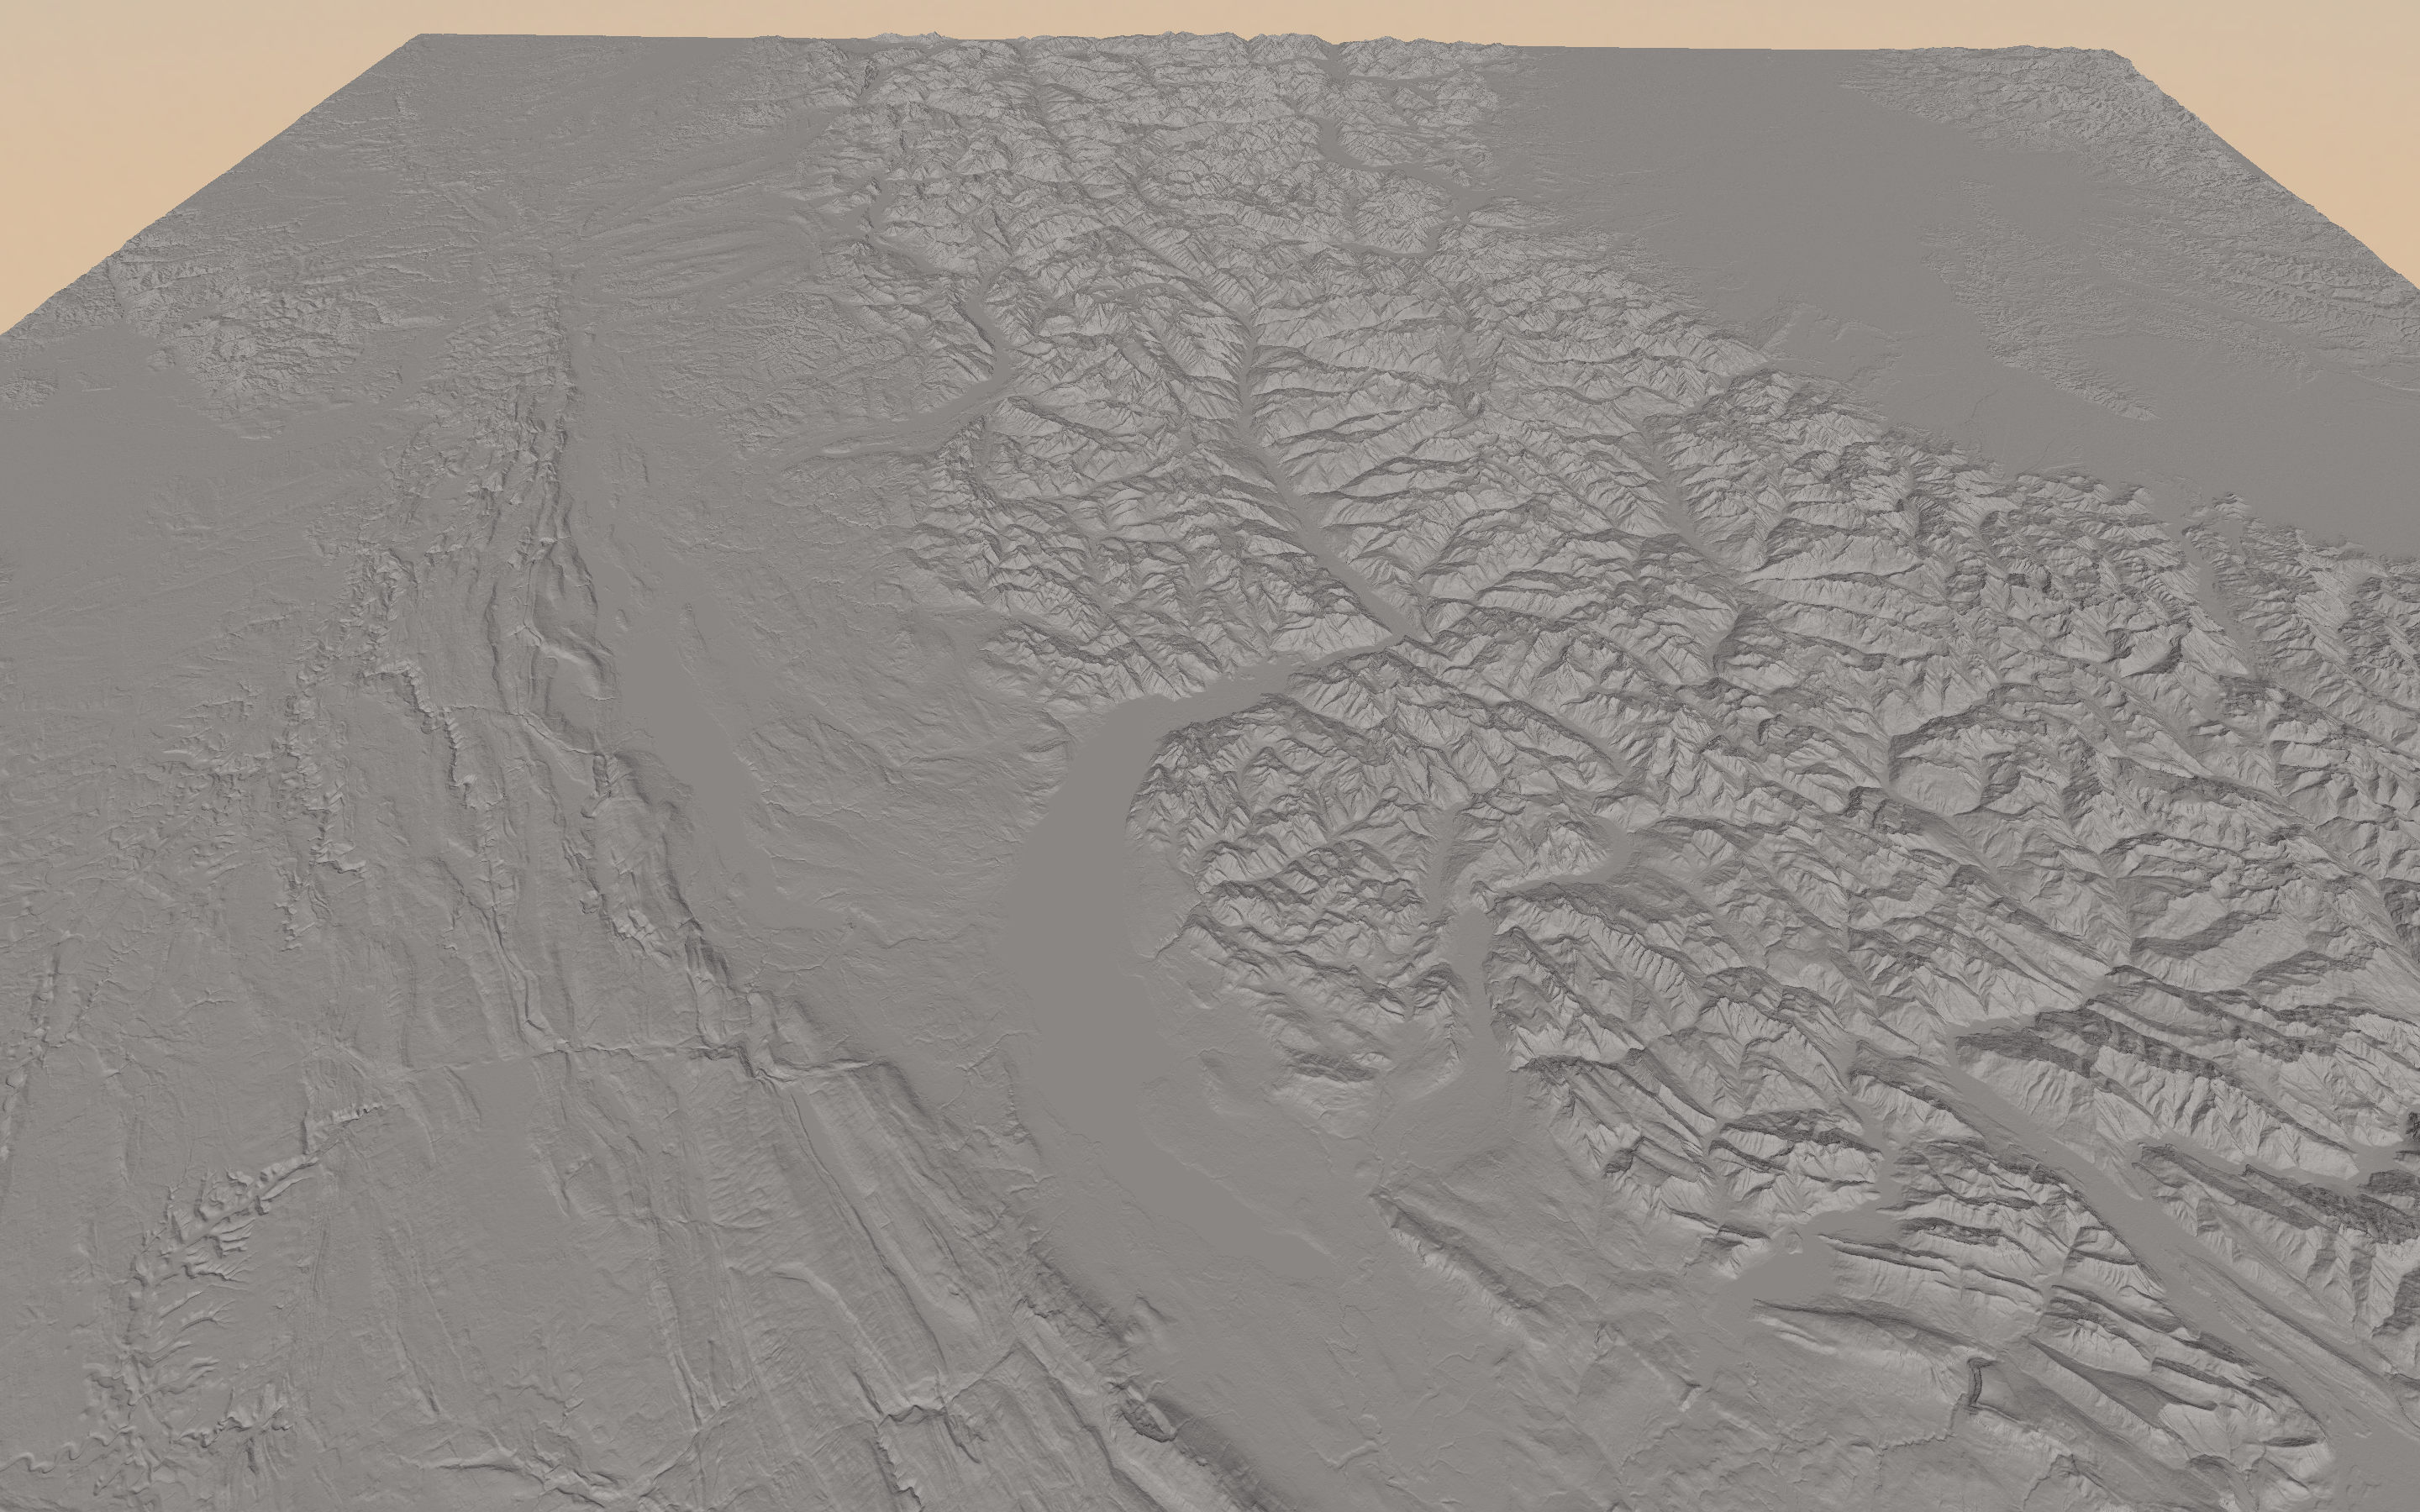
\includegraphics[width=0.4\textwidth]{results-accuracy-large-1-no-lod} }}
  \qquad
  \subfloat[\centering With LOD.]{{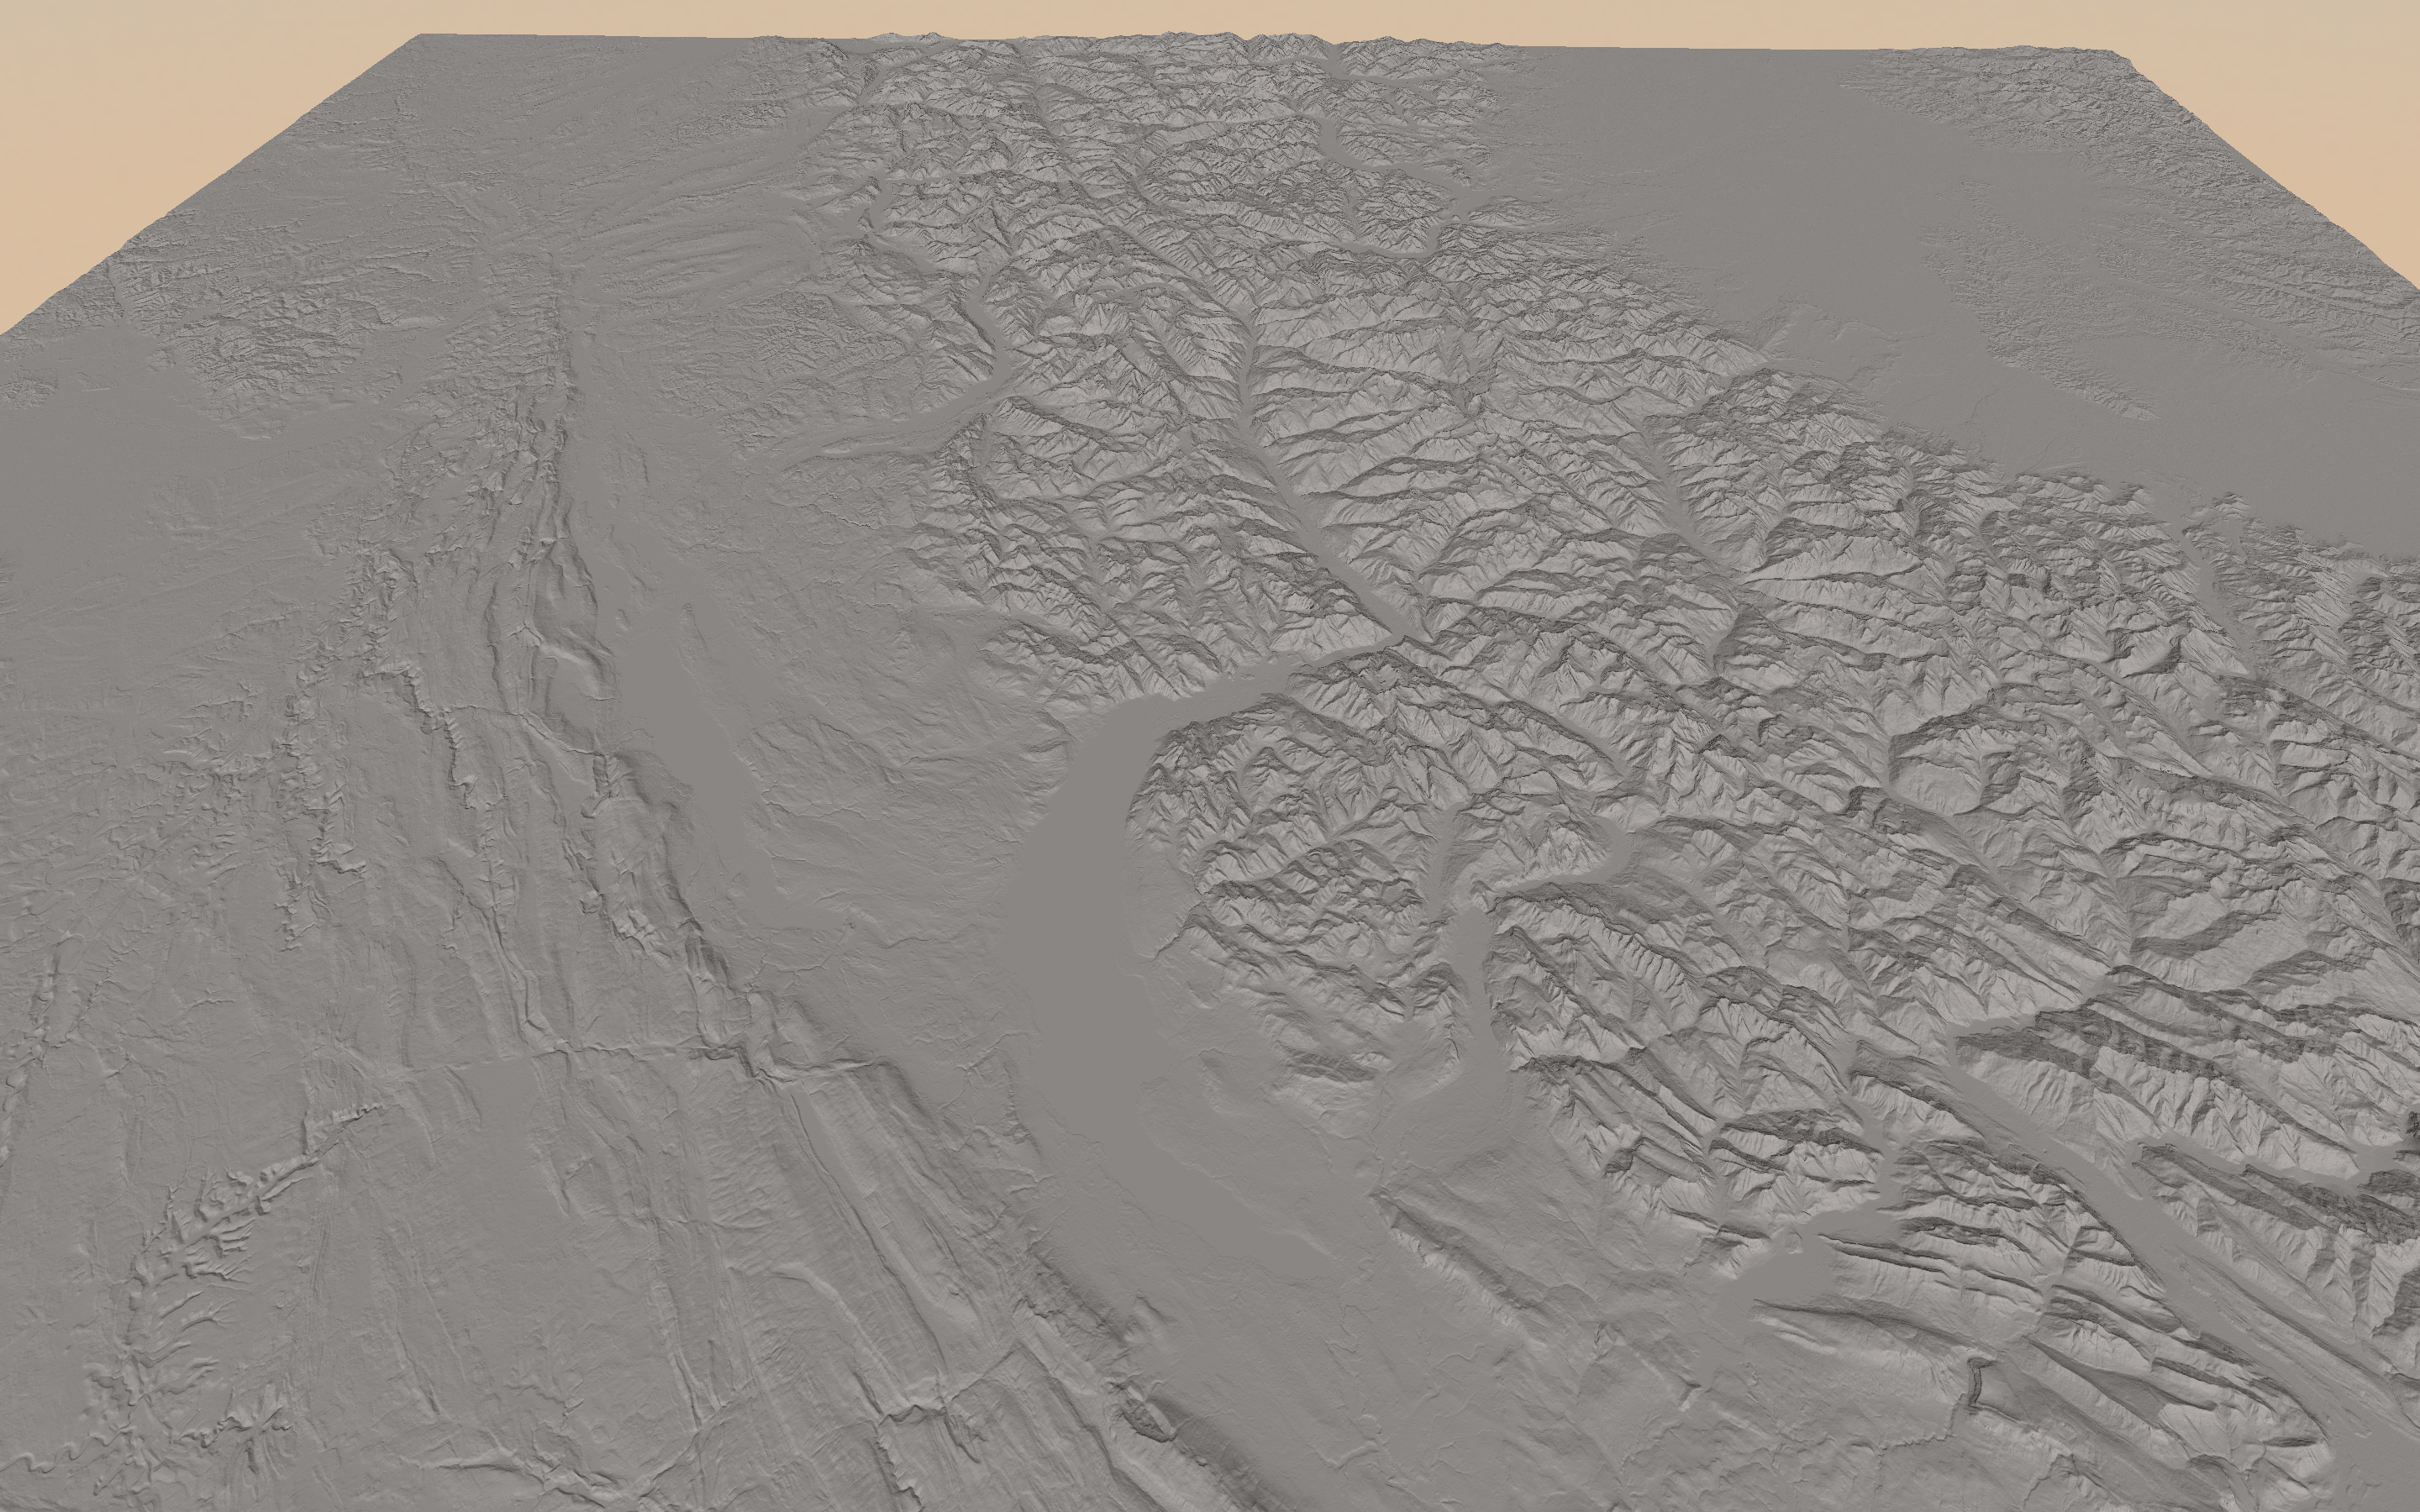
\includegraphics[width=0.4\textwidth]{results-accuracy-large-1-lod} }}
  \qquad
  \subfloat[\centering Absolute difference.]{{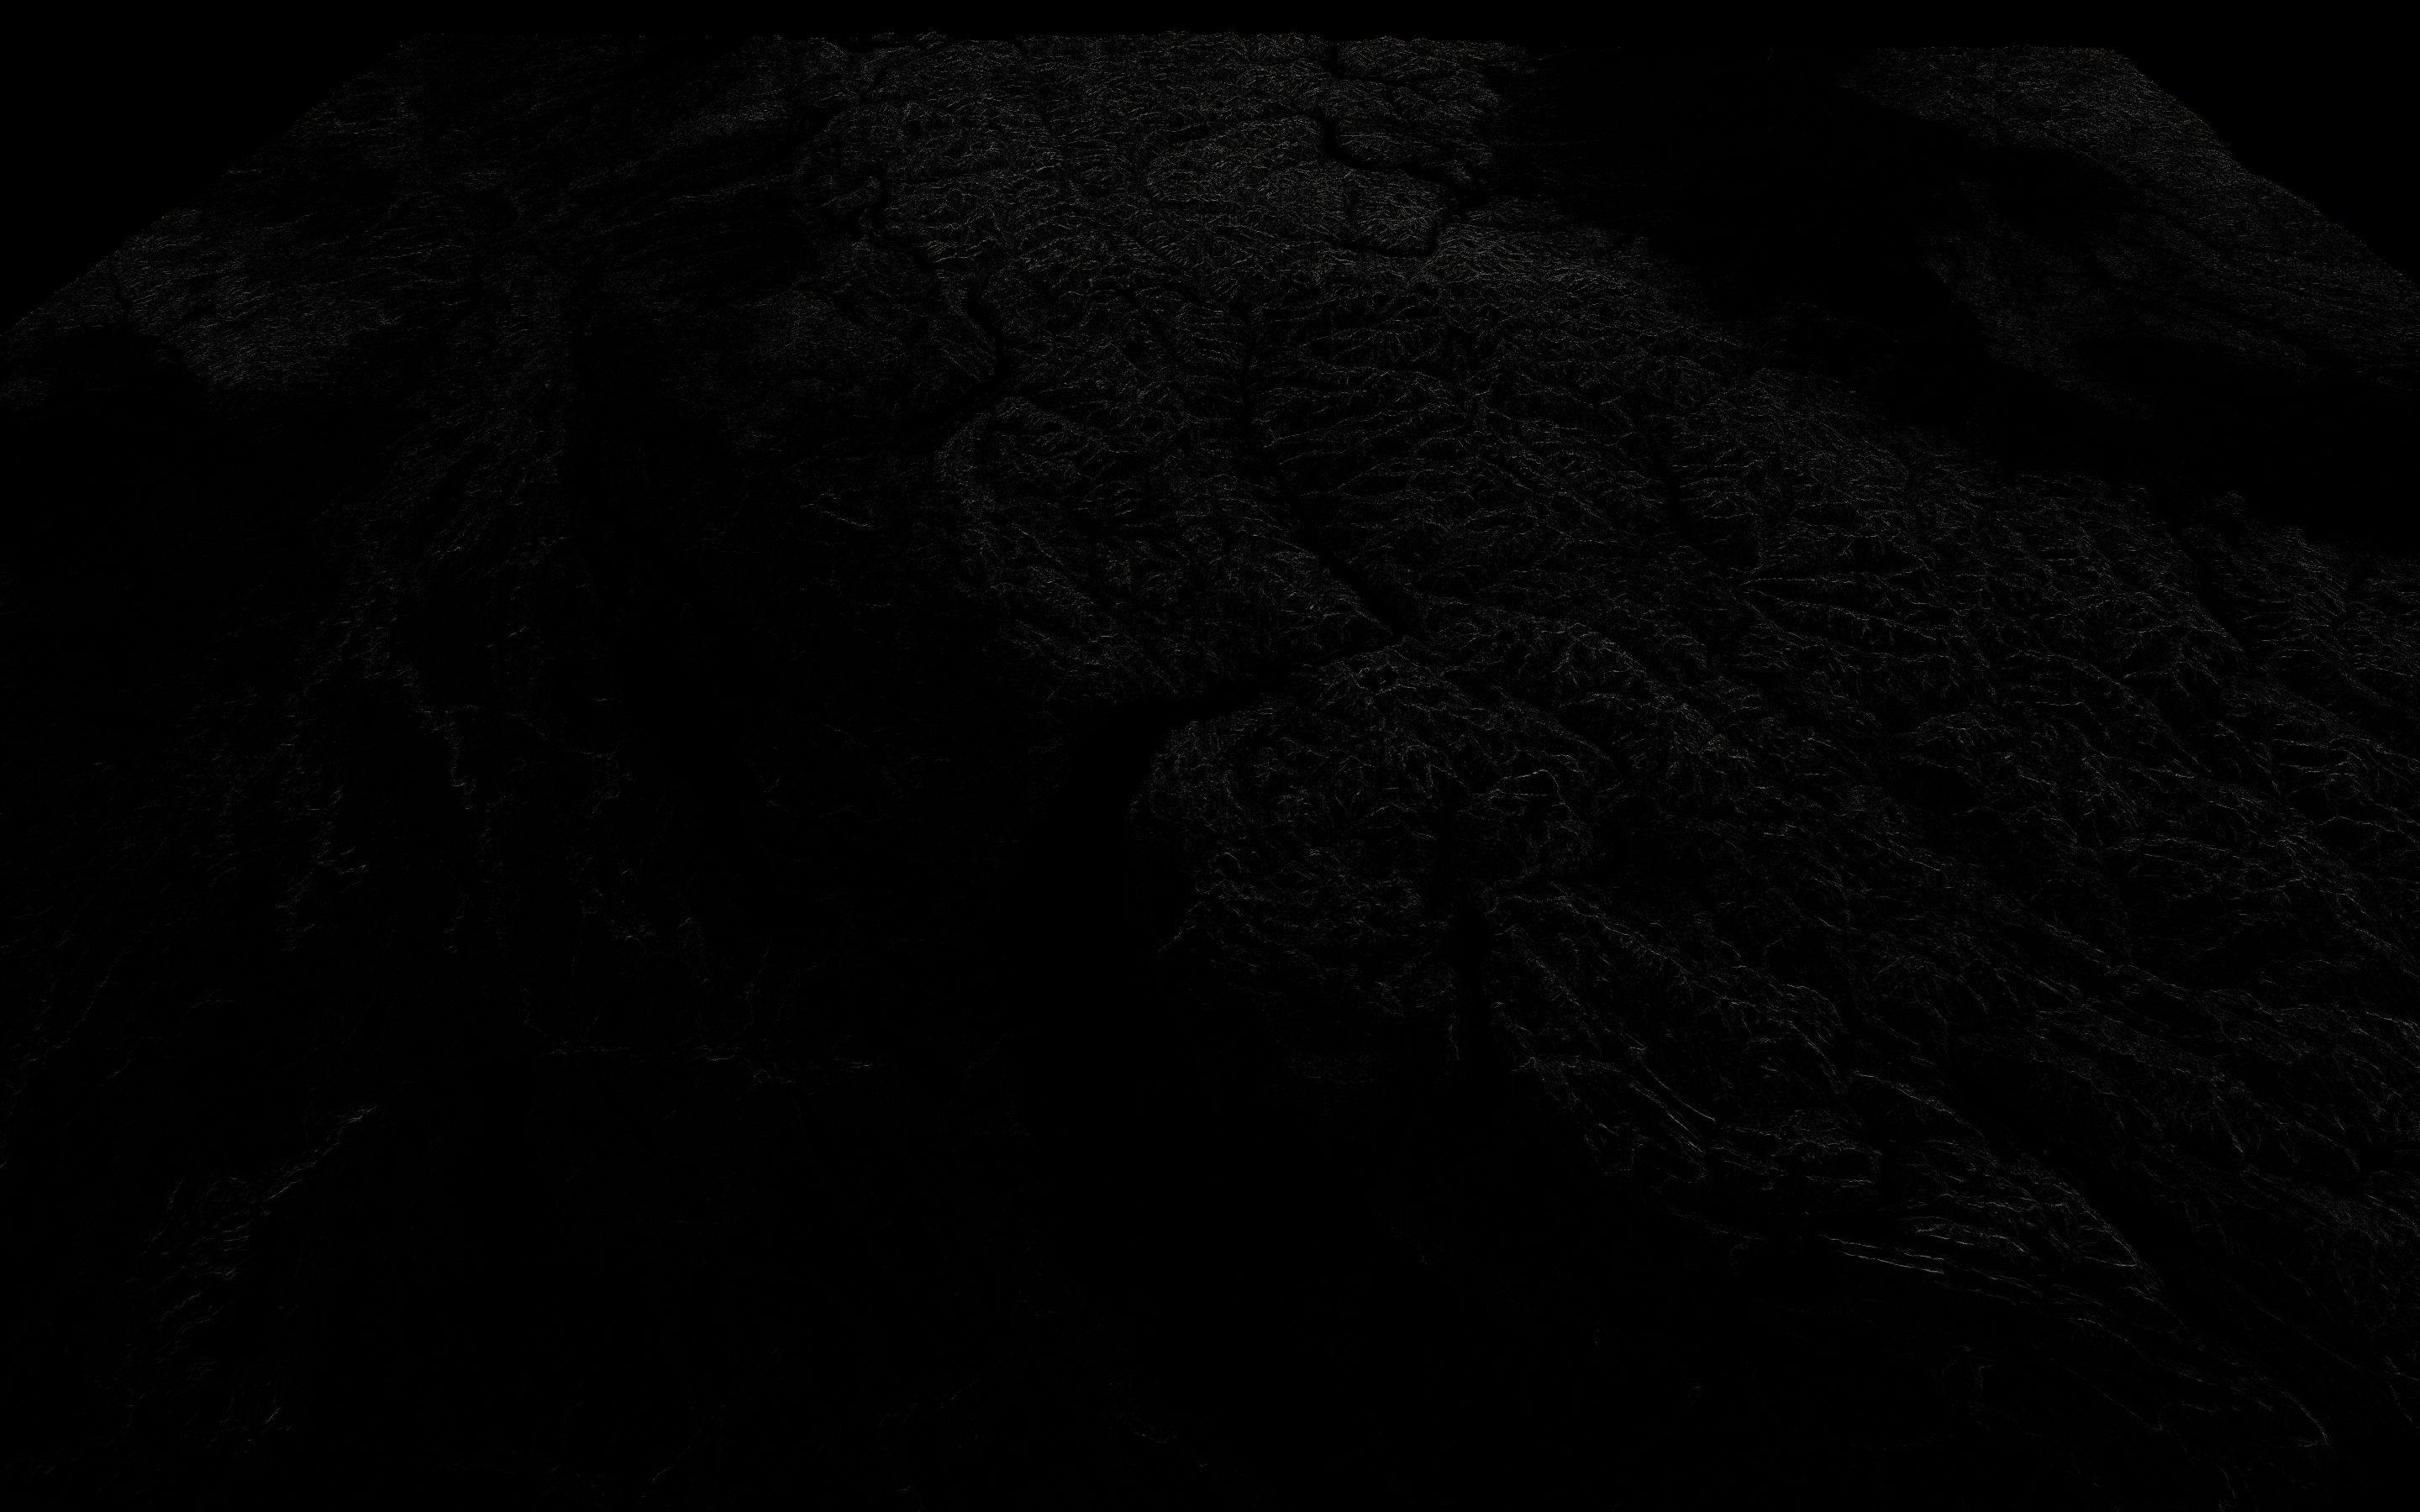
\includegraphics[width=0.4\textwidth]{results-accuracy-large-1-diff} }}
  \qquad
  \subfloat[\centering Absolute difference (binarised).]{{\includegraphics[width=0.4\textwidth]{results-accuracy-large-1-diff-bin} }}
  \caption{Screenshot showcasing the screenshot of a large section of the terrain with no LOD (a), with LOD (b),
   the absolute difference (c) between (a) and (b), and the binarised absolute difference (d) of (c). The computed RMSE is 3.94.}\label{fig:results-large-1}
\end{figure}
\subsubsection{Large Terrain Screenshot 2}
\begin{figure}[H]
  \centering
  \subfloat[\centering No LOD.]{{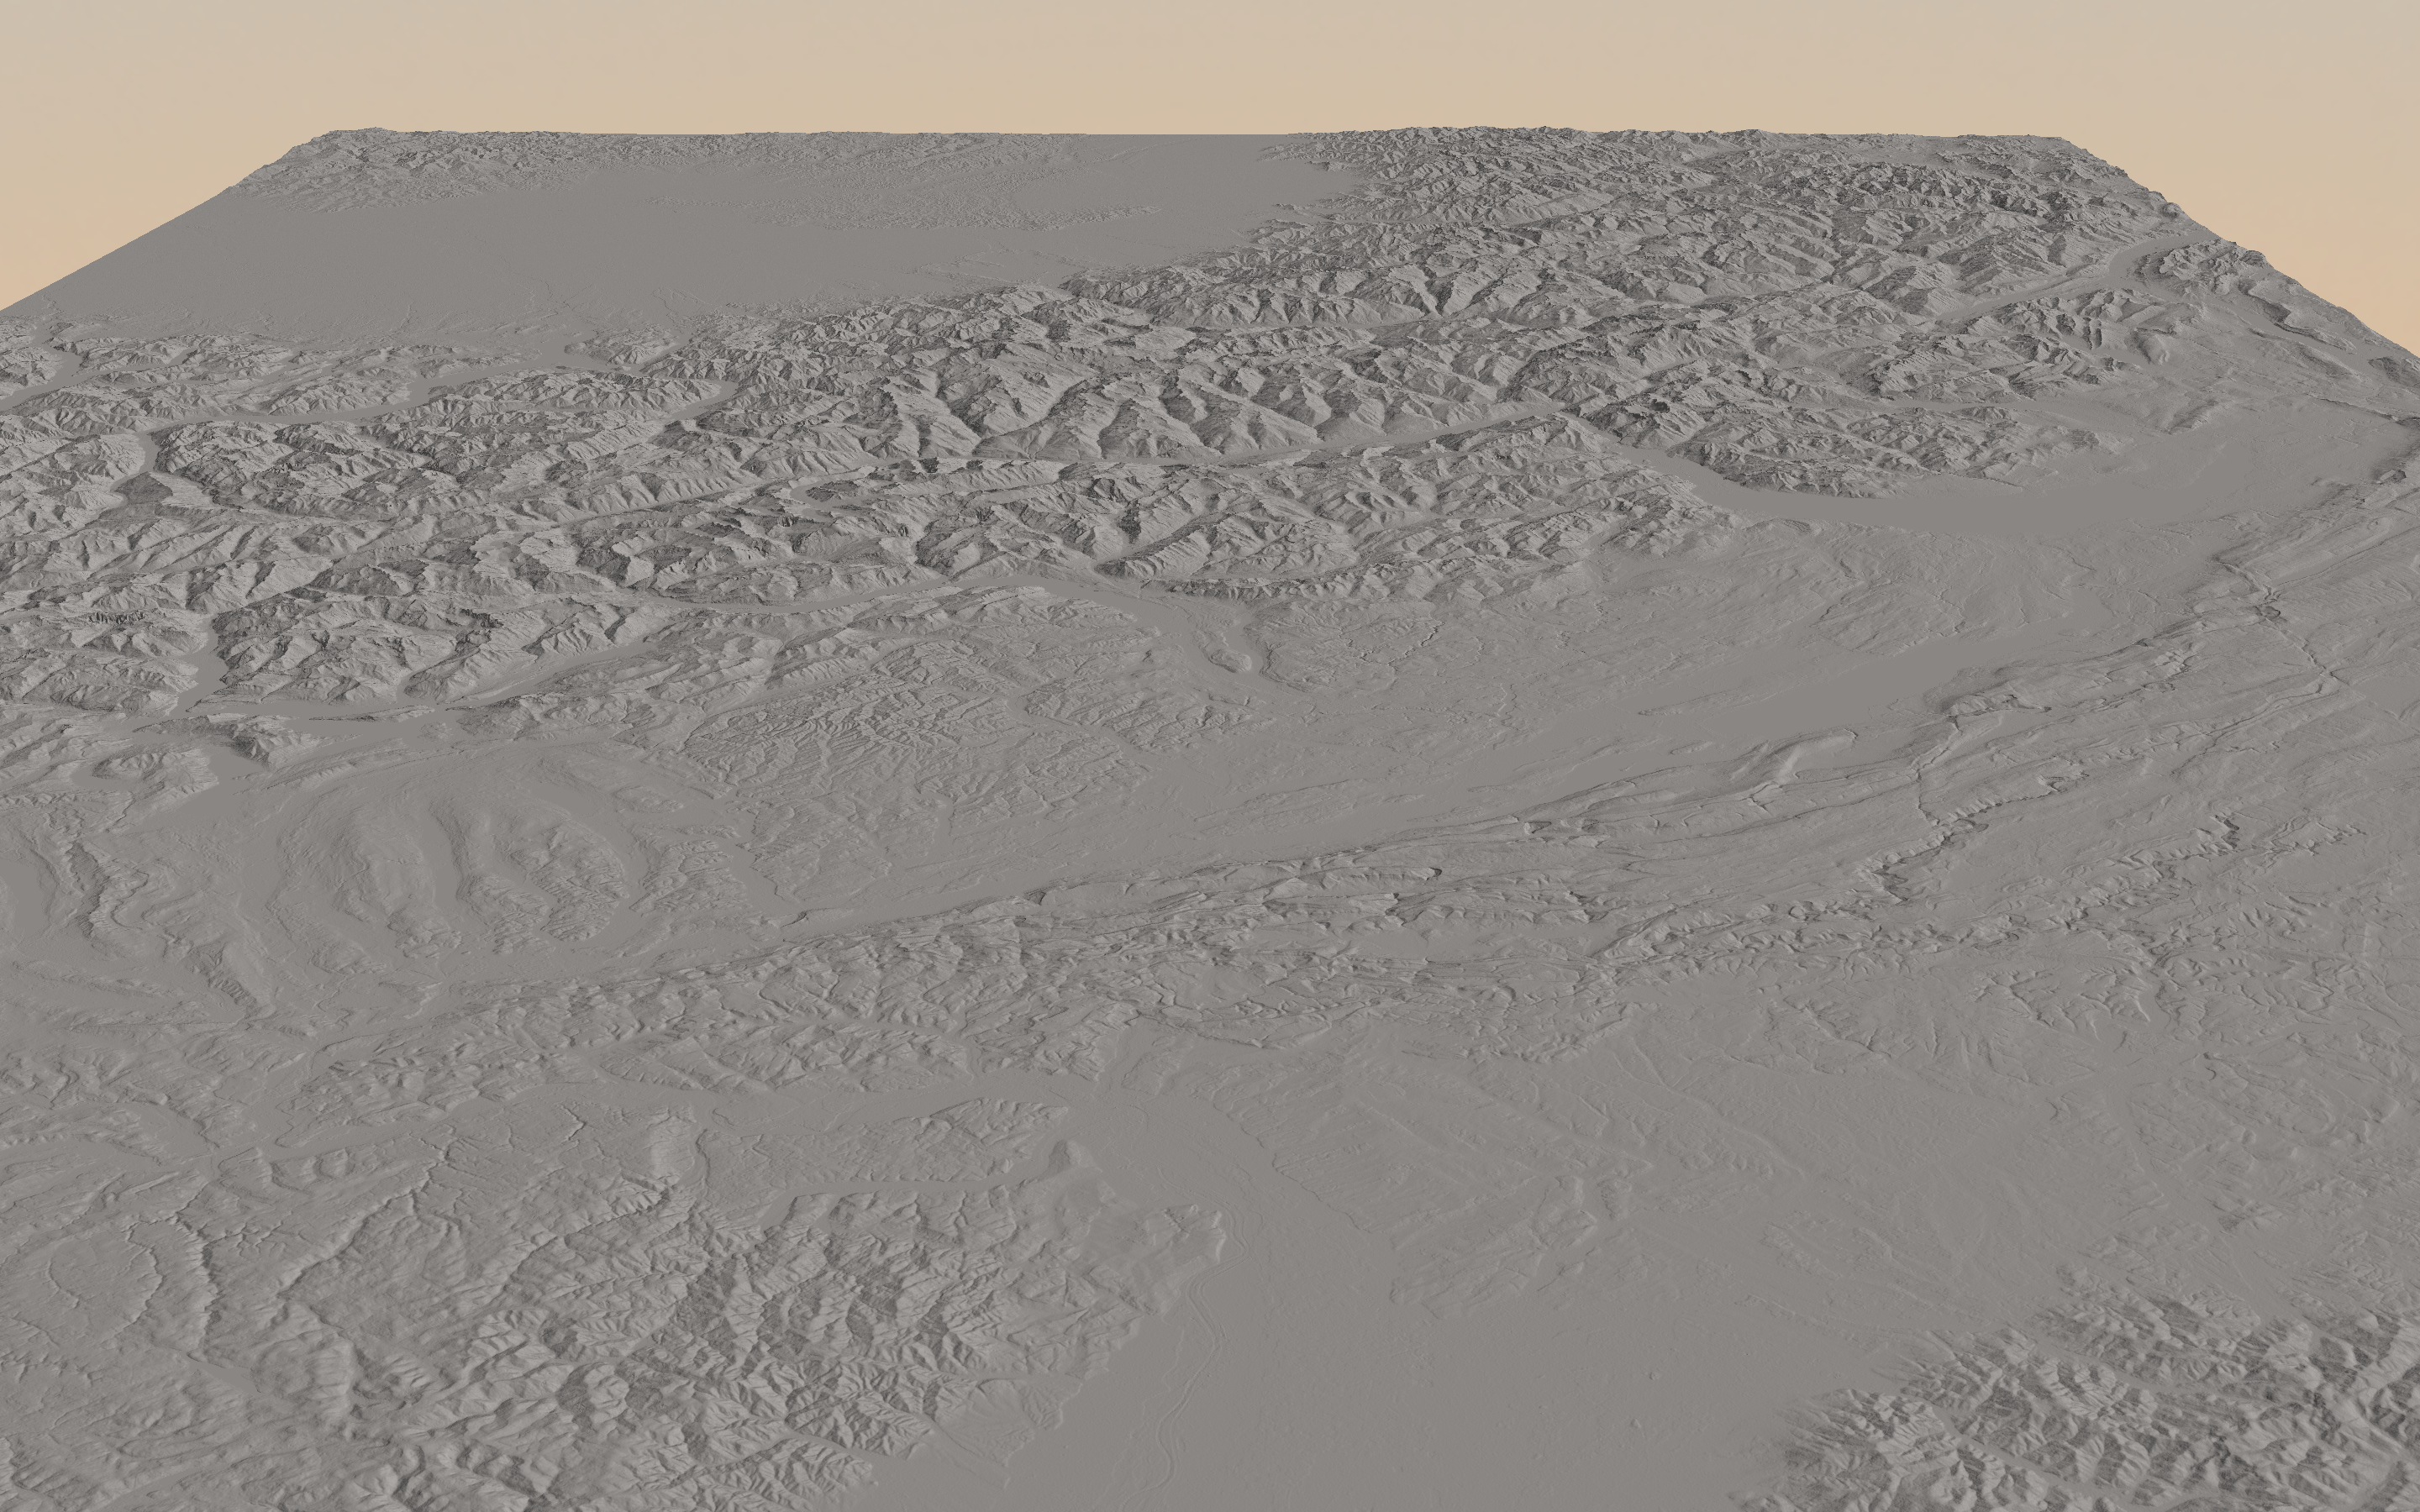
\includegraphics[width=0.4\textwidth]{results-accuracy-large-2-no-lod} }}
  \qquad
  \subfloat[\centering With LOD.]{{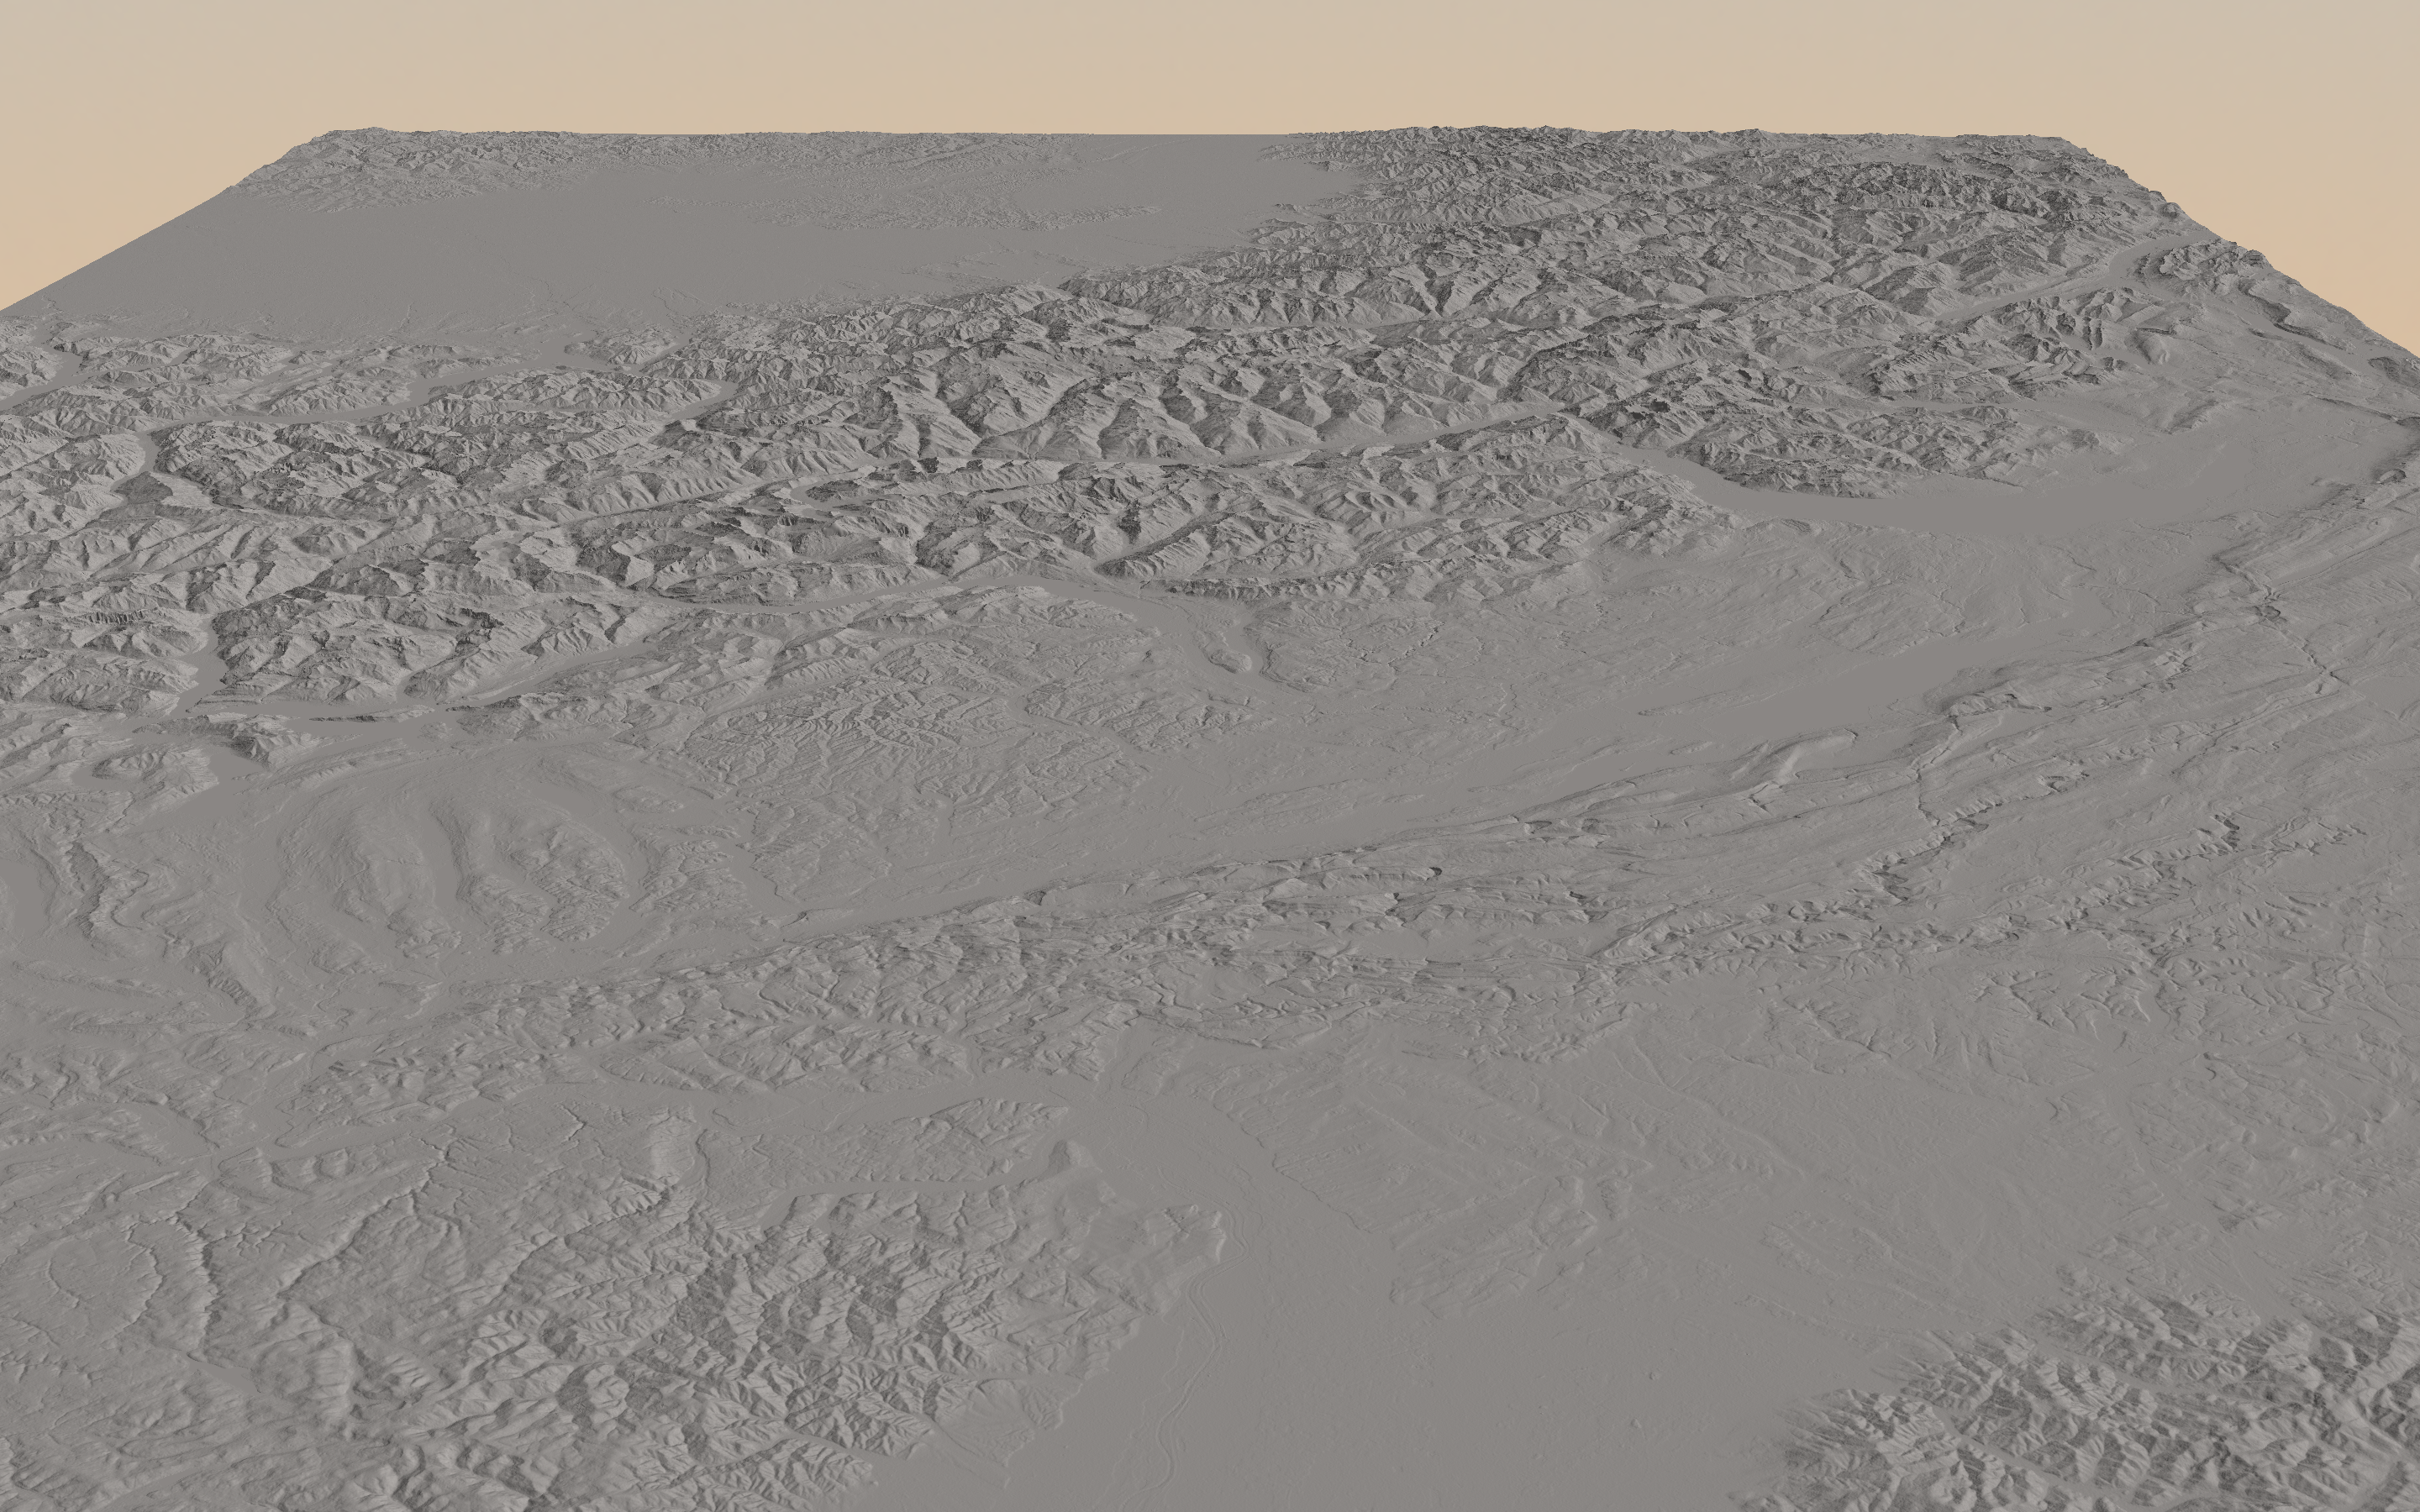
\includegraphics[width=0.4\textwidth]{results-accuracy-large-2-lod} }}
  \qquad
  \subfloat[\centering Absolute difference.]{{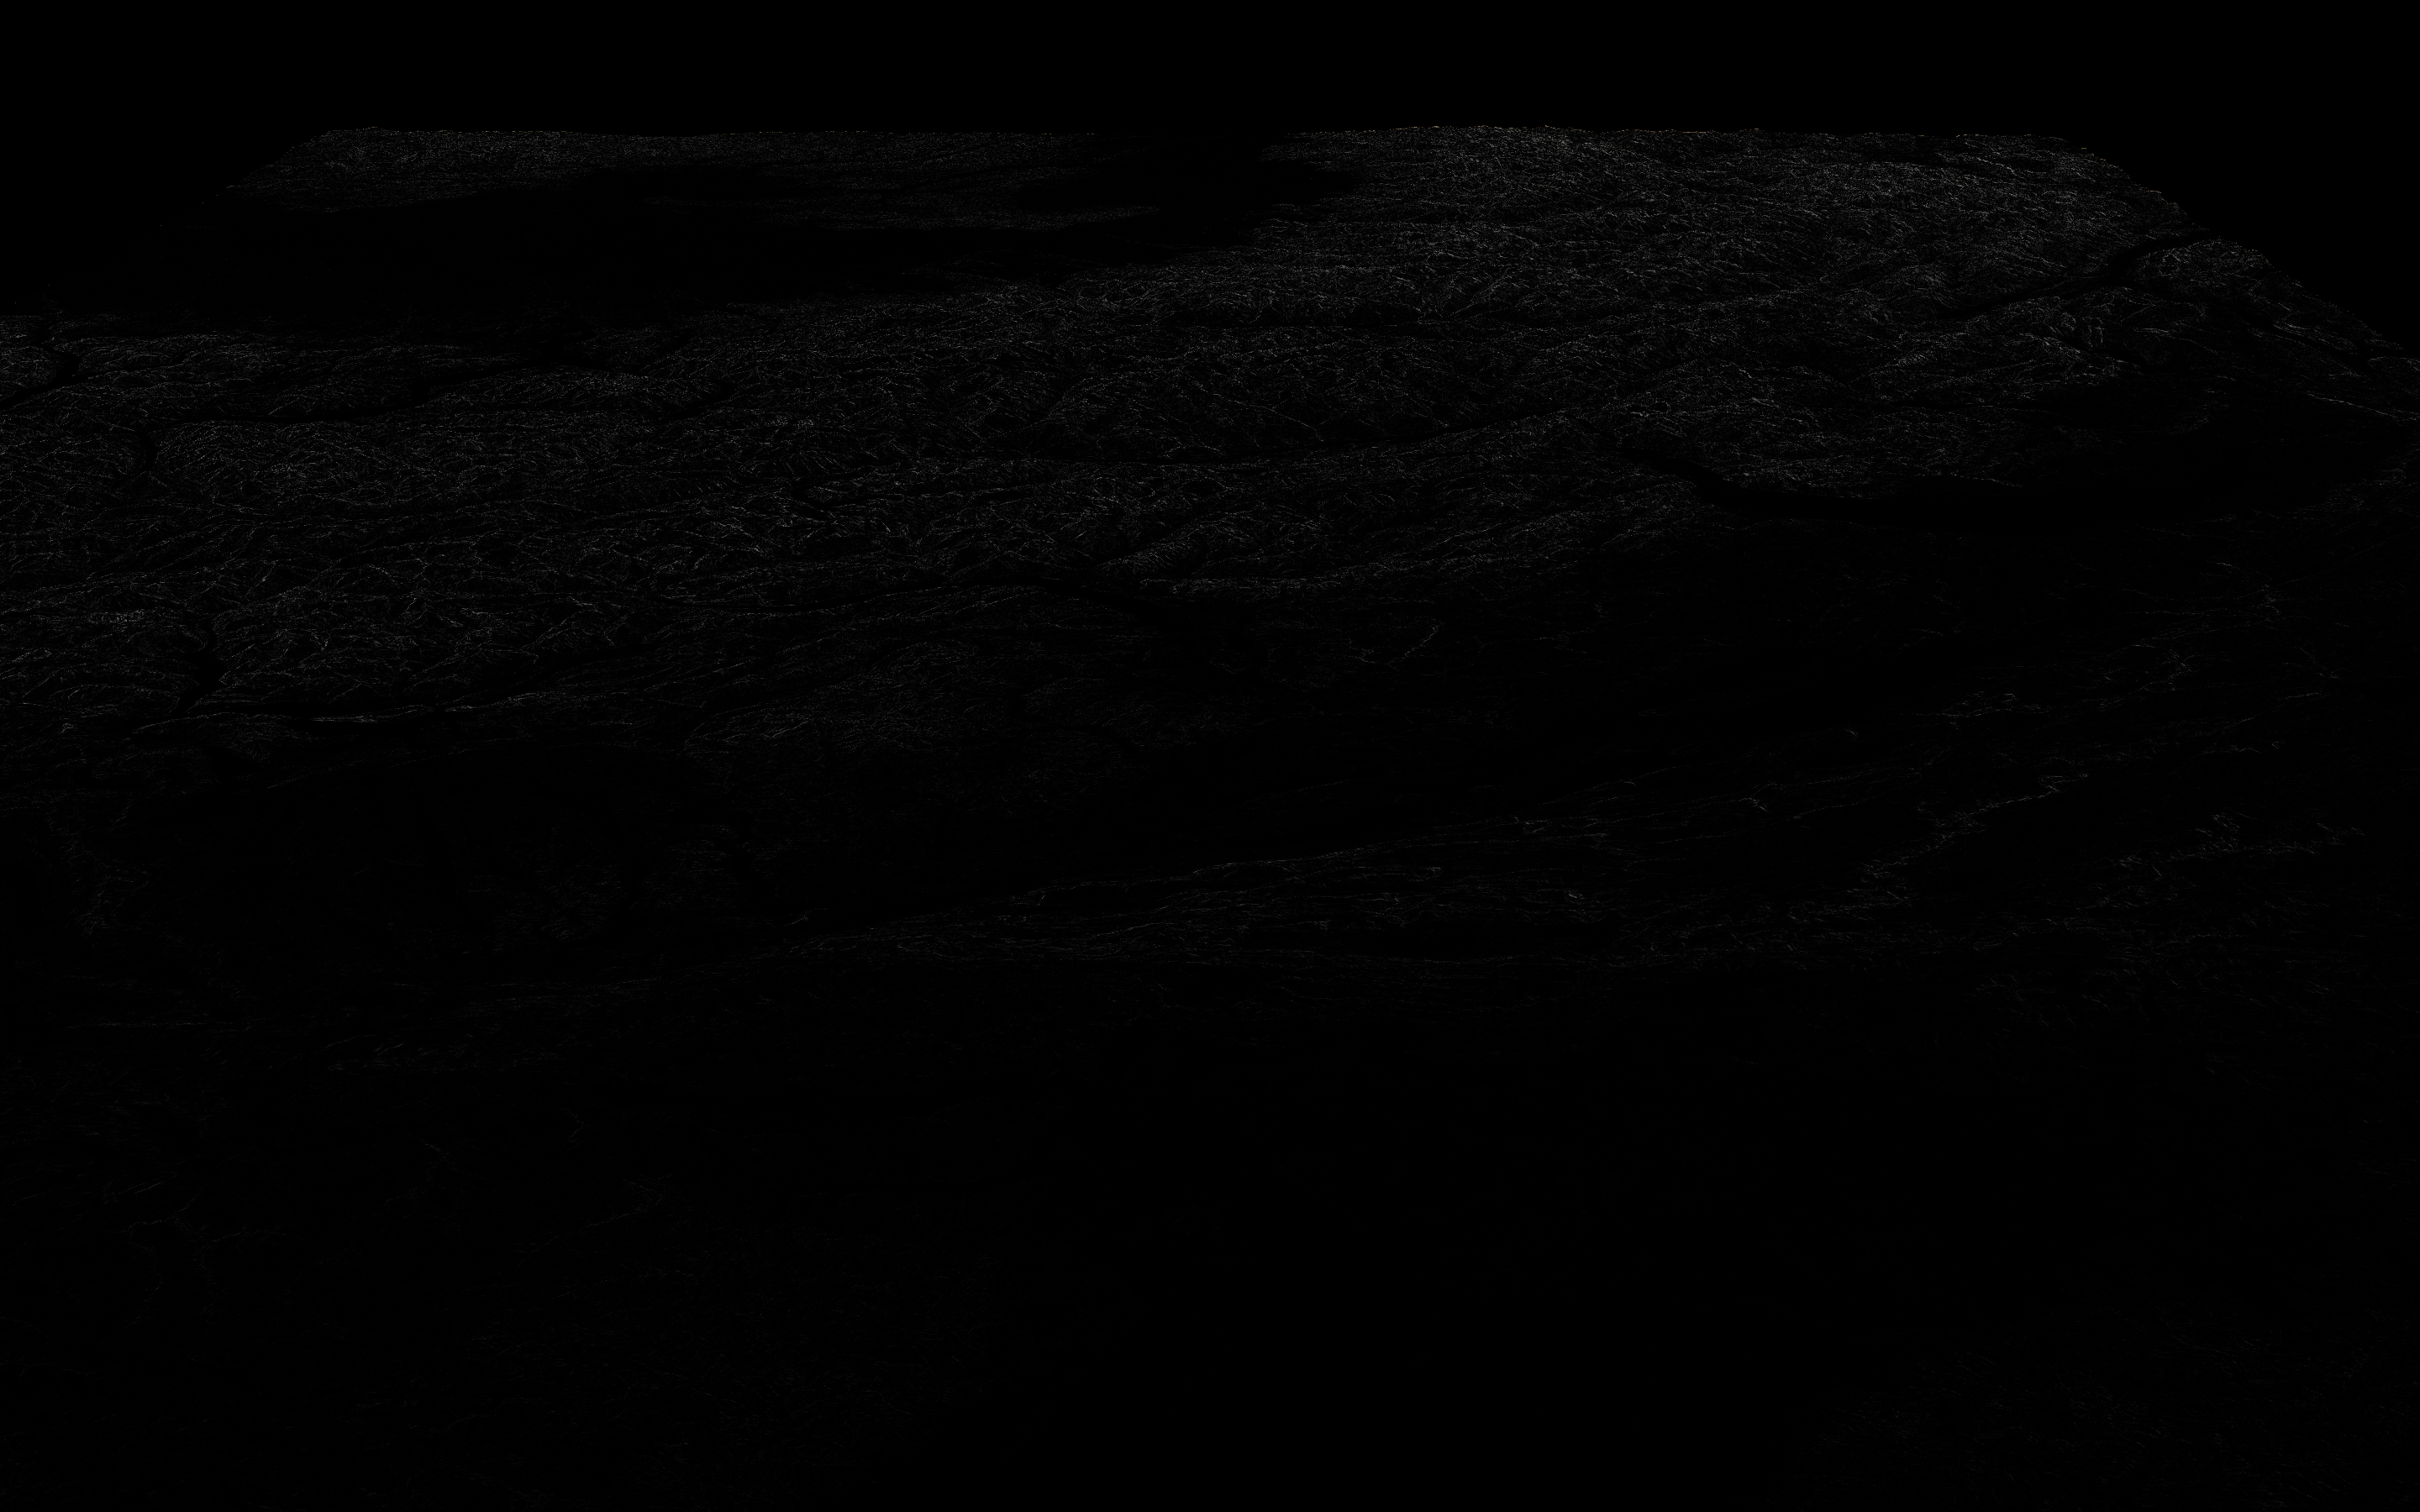
\includegraphics[width=0.4\textwidth]{results-accuracy-large-2-diff} }}
  \qquad
  \subfloat[\centering Absolute difference (binarised).]{{\includegraphics[width=0.4\textwidth]{results-accuracy-large-2-diff-bin} }}
  \caption{Screenshot showcasing the screenshot of a large section of the terrain with no LOD (a), with LOD (b),
   the absolute difference (c) between (a) and (b), and the binarised absolute difference (d) of (c). The computed RMSE is 3.1.}\label{fig:results-large-2}
\end{figure}
\subsubsection{Large Terrain Screenshot 3}
\begin{figure}[H]
  \centering
  \subfloat[\centering No LOD.]{{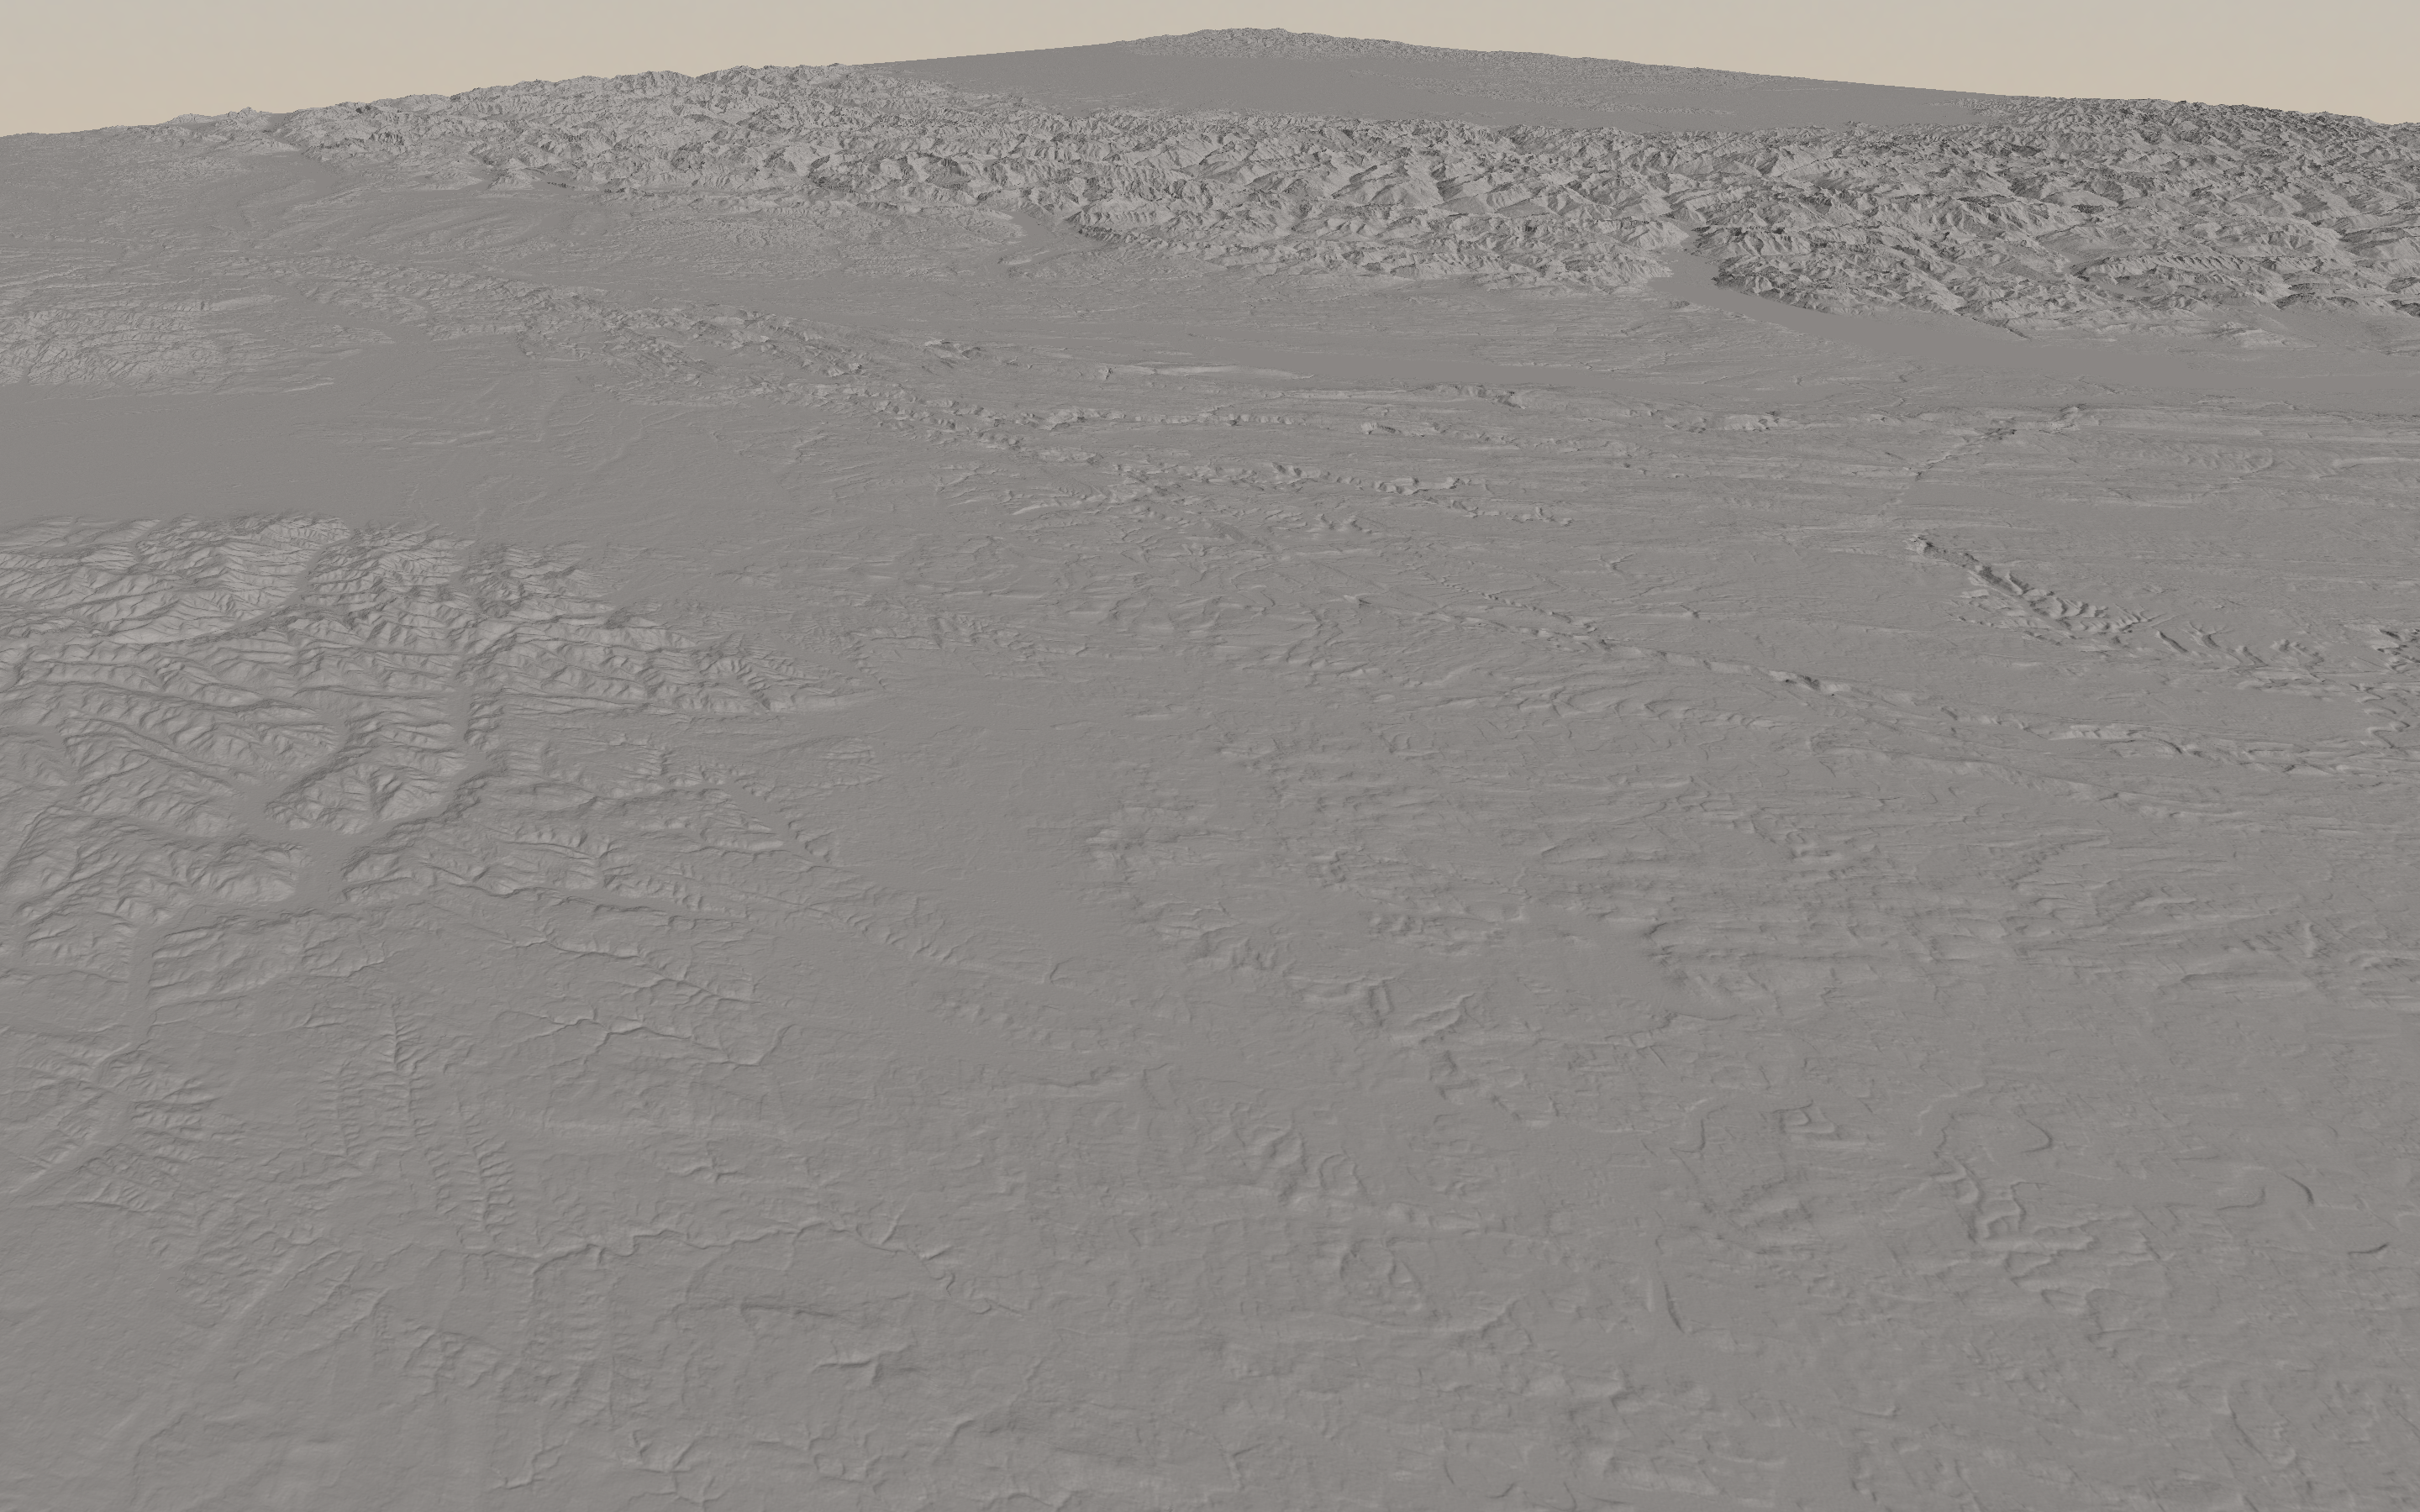
\includegraphics[width=0.4\textwidth]{results-accuracy-large-3-no-lod} }}
  \qquad
  \subfloat[\centering With LOD.]{{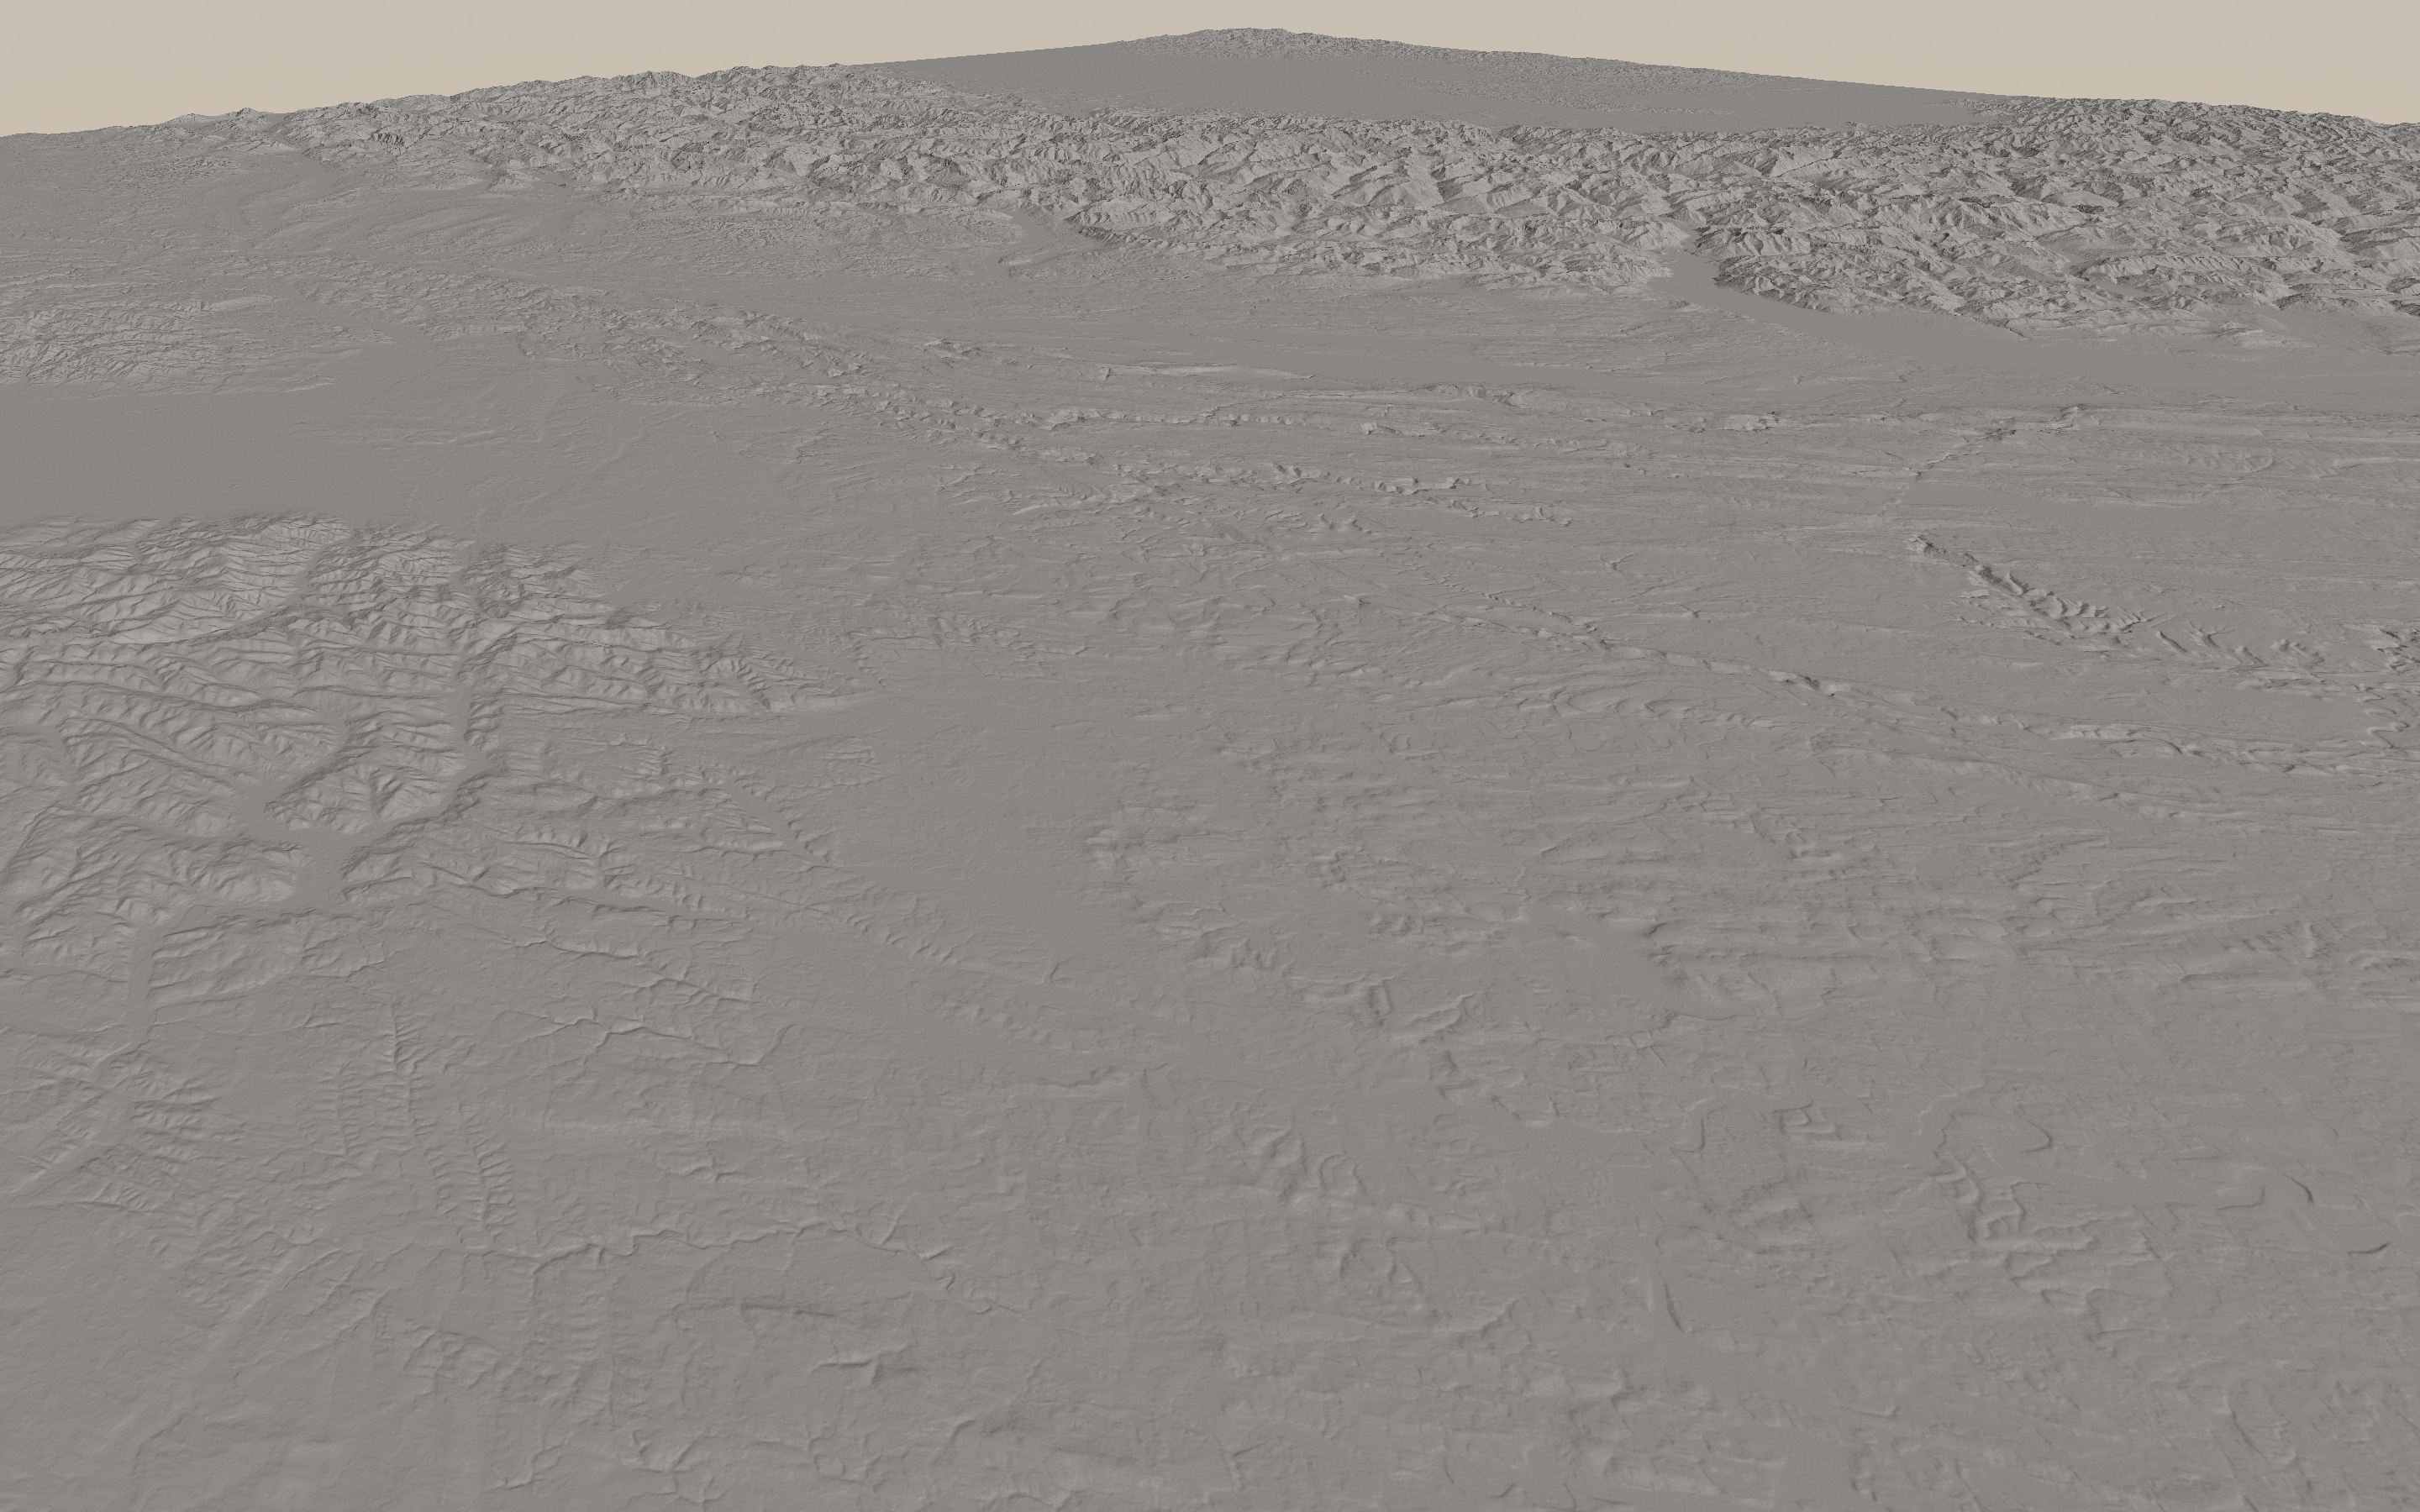
\includegraphics[width=0.4\textwidth]{results-accuracy-large-3-lod} }}
  \qquad
  \subfloat[\centering Absolute difference.]{{\includegraphics[width=0.4\textwidth]{results-accuracy-large-3-diff} }}
  \qquad
  \subfloat[\centering Absolute difference (binarised).]{{\includegraphics[width=0.4\textwidth]{results-accuracy-large-3-diff-bin} }}
  \caption{Screenshot showcasing the screenshot of a large section of the terrain with no LOD (a), with LOD (b),
   the absolute difference (c) between (a) and (b), and the binarised absolute difference (d) of (c). The computed RMSE is 2.59.}\label{fig:results-large-3}
\end{figure}
\subsubsection{Large Terrain Screenshot 4}
\begin{figure}[H]
  \centering
  \subfloat[\centering No LOD.]{{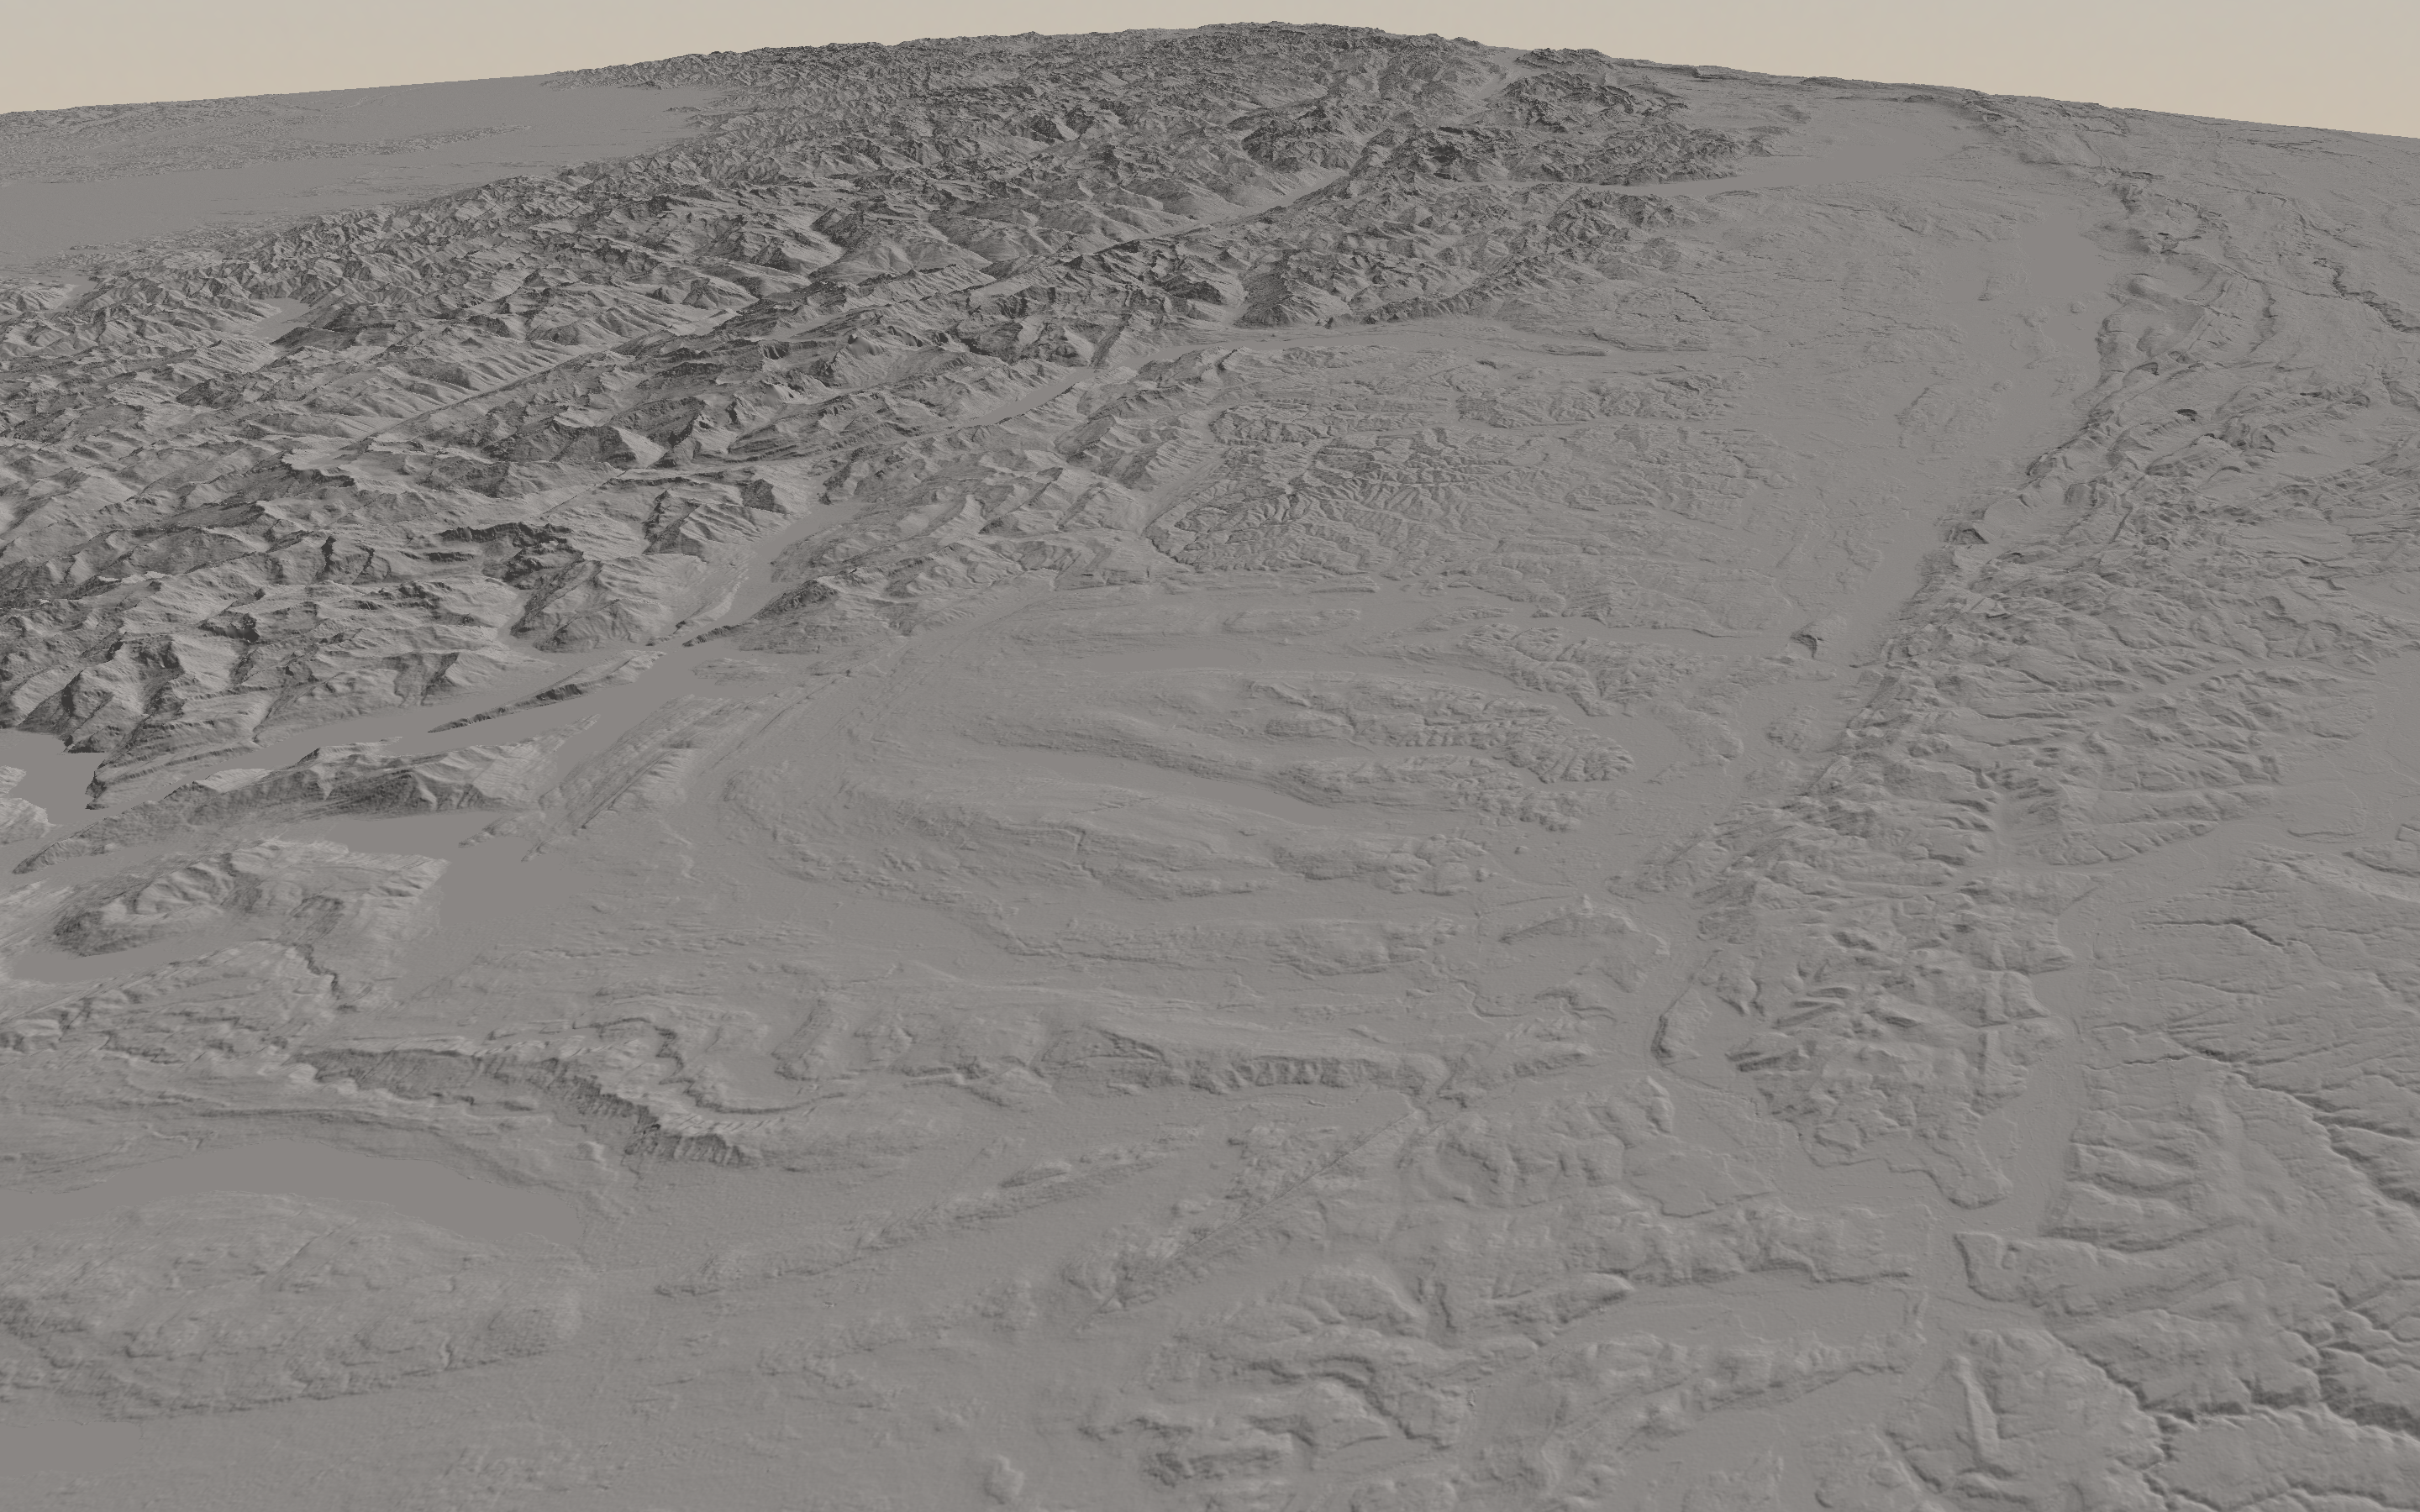
\includegraphics[width=0.4\textwidth]{results-accuracy-large-4-no-lod} }}
  \qquad
  \subfloat[\centering With LOD.]{{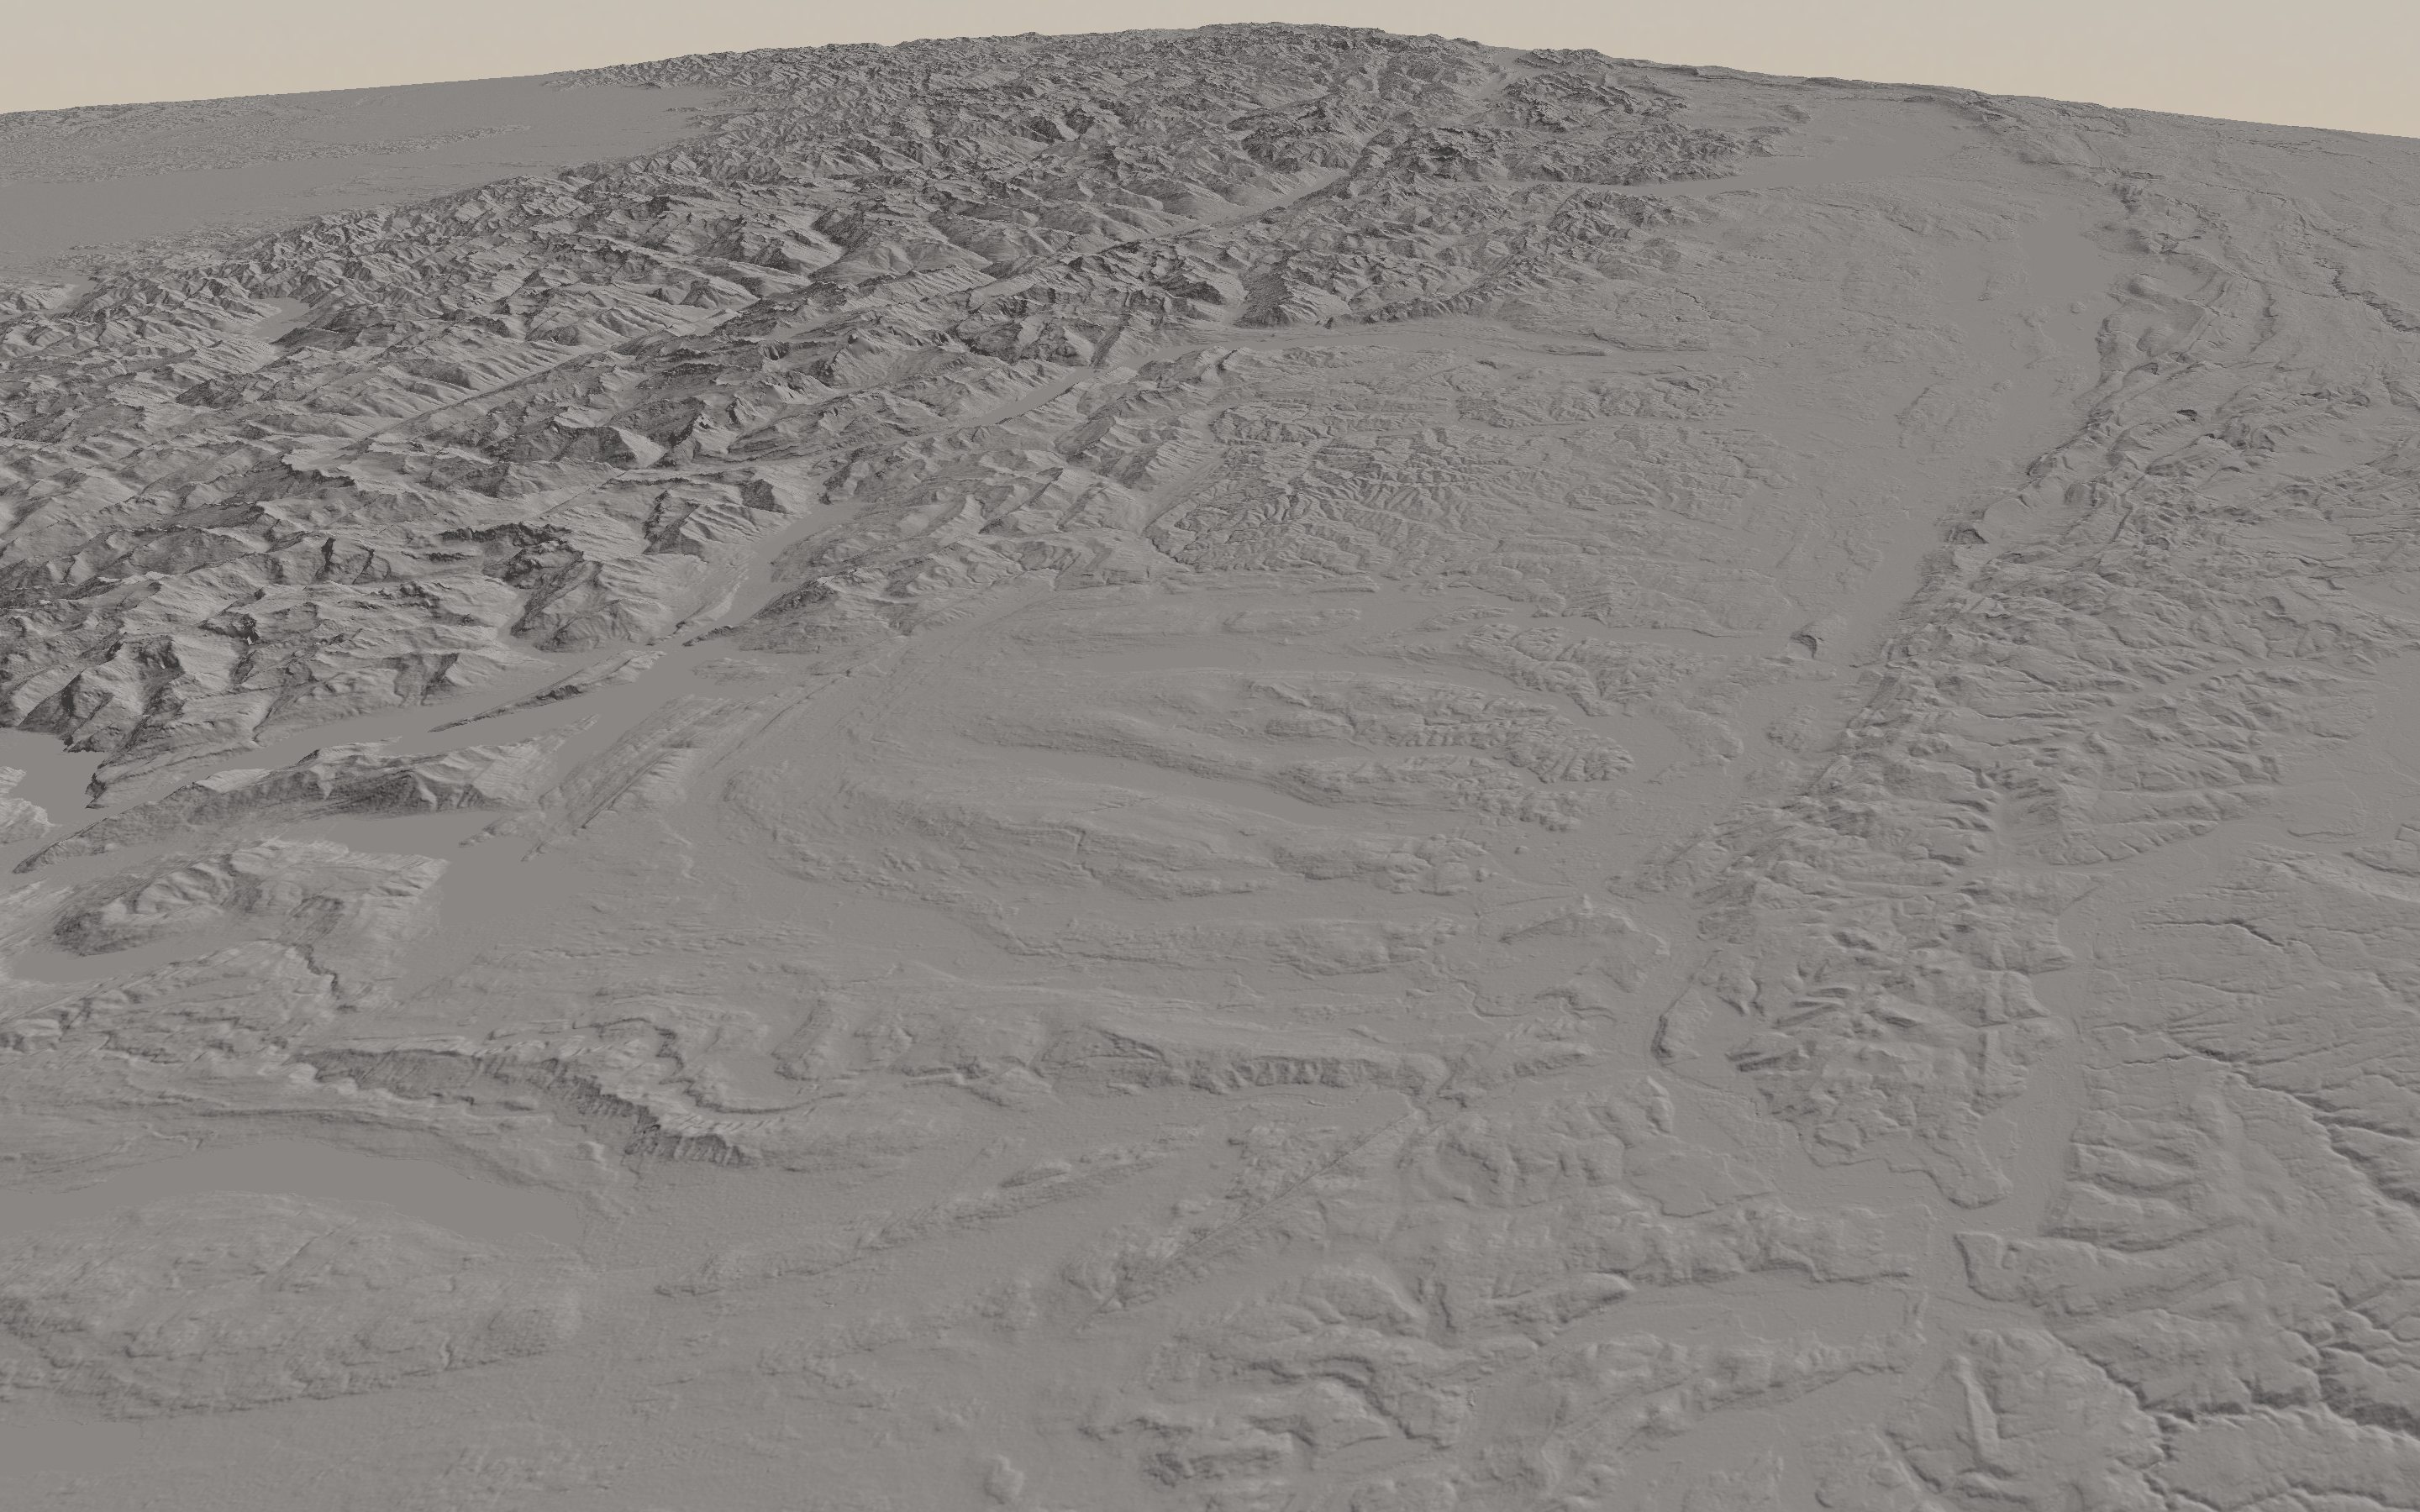
\includegraphics[width=0.4\textwidth]{results-accuracy-large-4-lod} }}
  \qquad
  \subfloat[\centering Absolute difference.]{{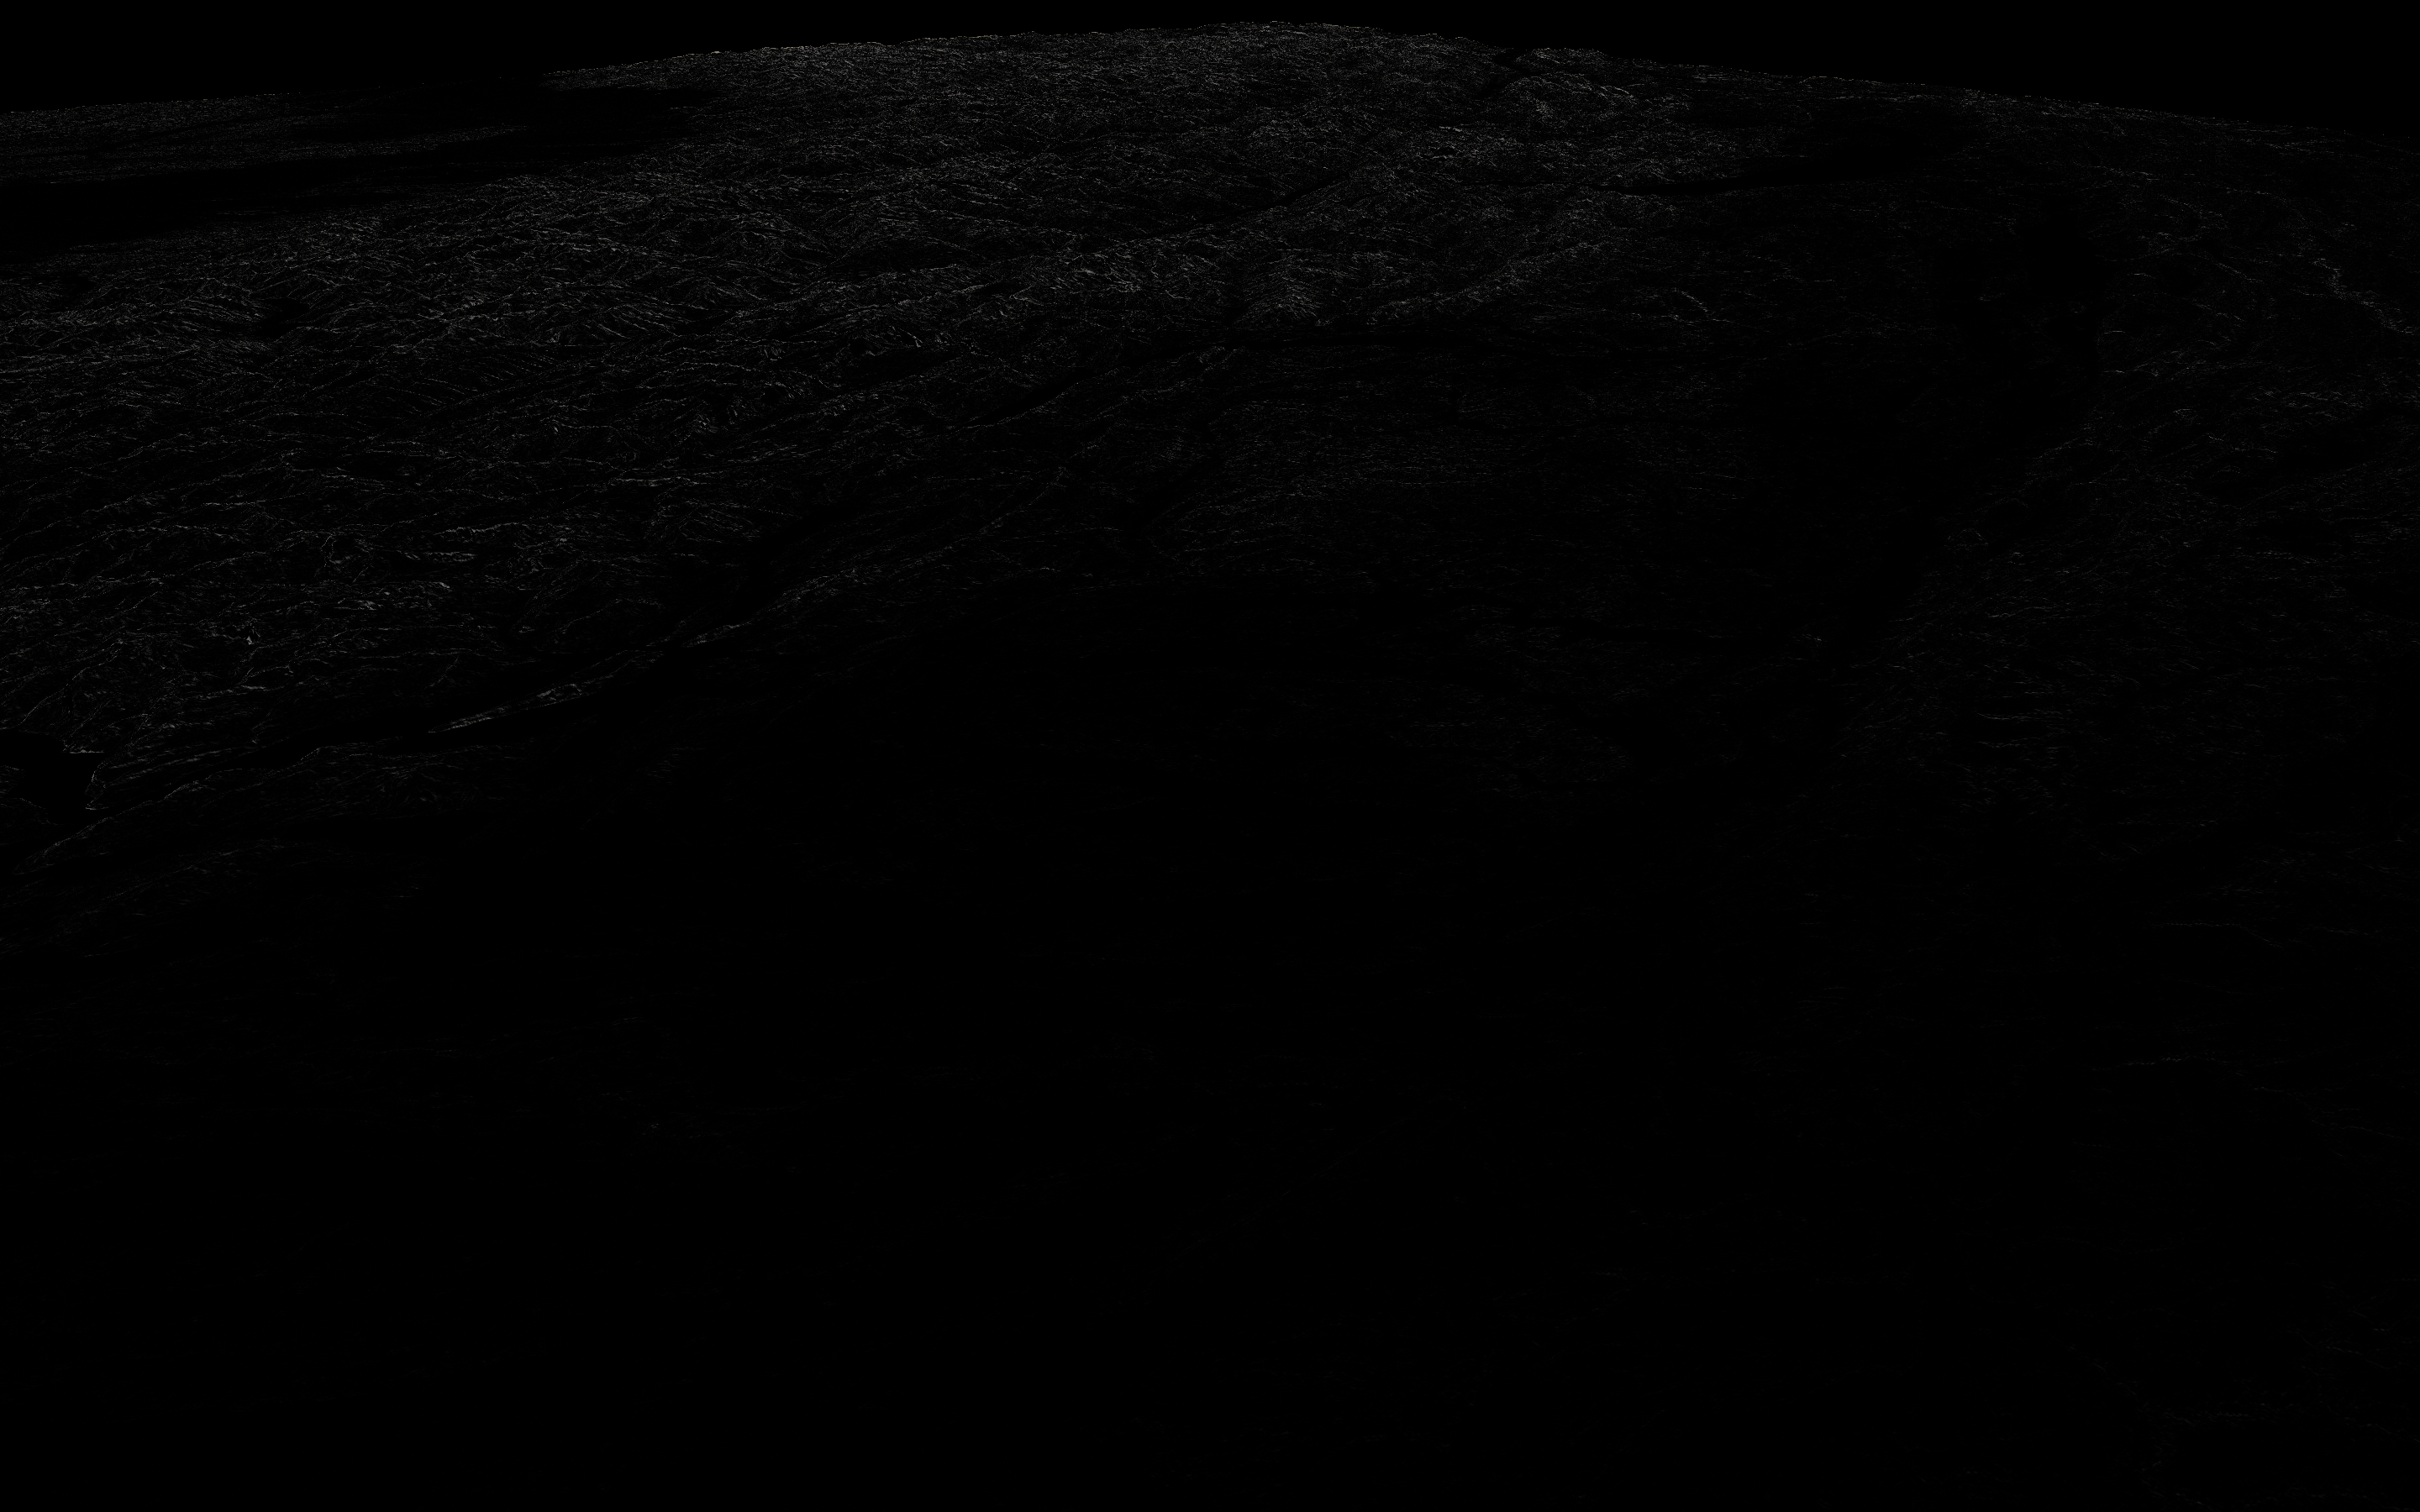
\includegraphics[width=0.4\textwidth]{results-accuracy-large-4-diff} }}
  \qquad
  \subfloat[\centering Absolute difference (binarised).]{{\includegraphics[width=0.4\textwidth]{results-accuracy-large-4-diff-bin} }}
  \caption{Screenshot showcasing the screenshot of a large section of the terrain with no LOD (a), with LOD (b),
   the absolute difference (c) between (a) and (b), and the binarised absolute difference (d) of (c). The computed RMSE is 1.96.}\label{fig:results-large-4}
\end{figure}
\subsubsection{Large Terrain Screenshot 5}
\begin{figure}[H]
  \centering
  \subfloat[\centering No LOD.]{{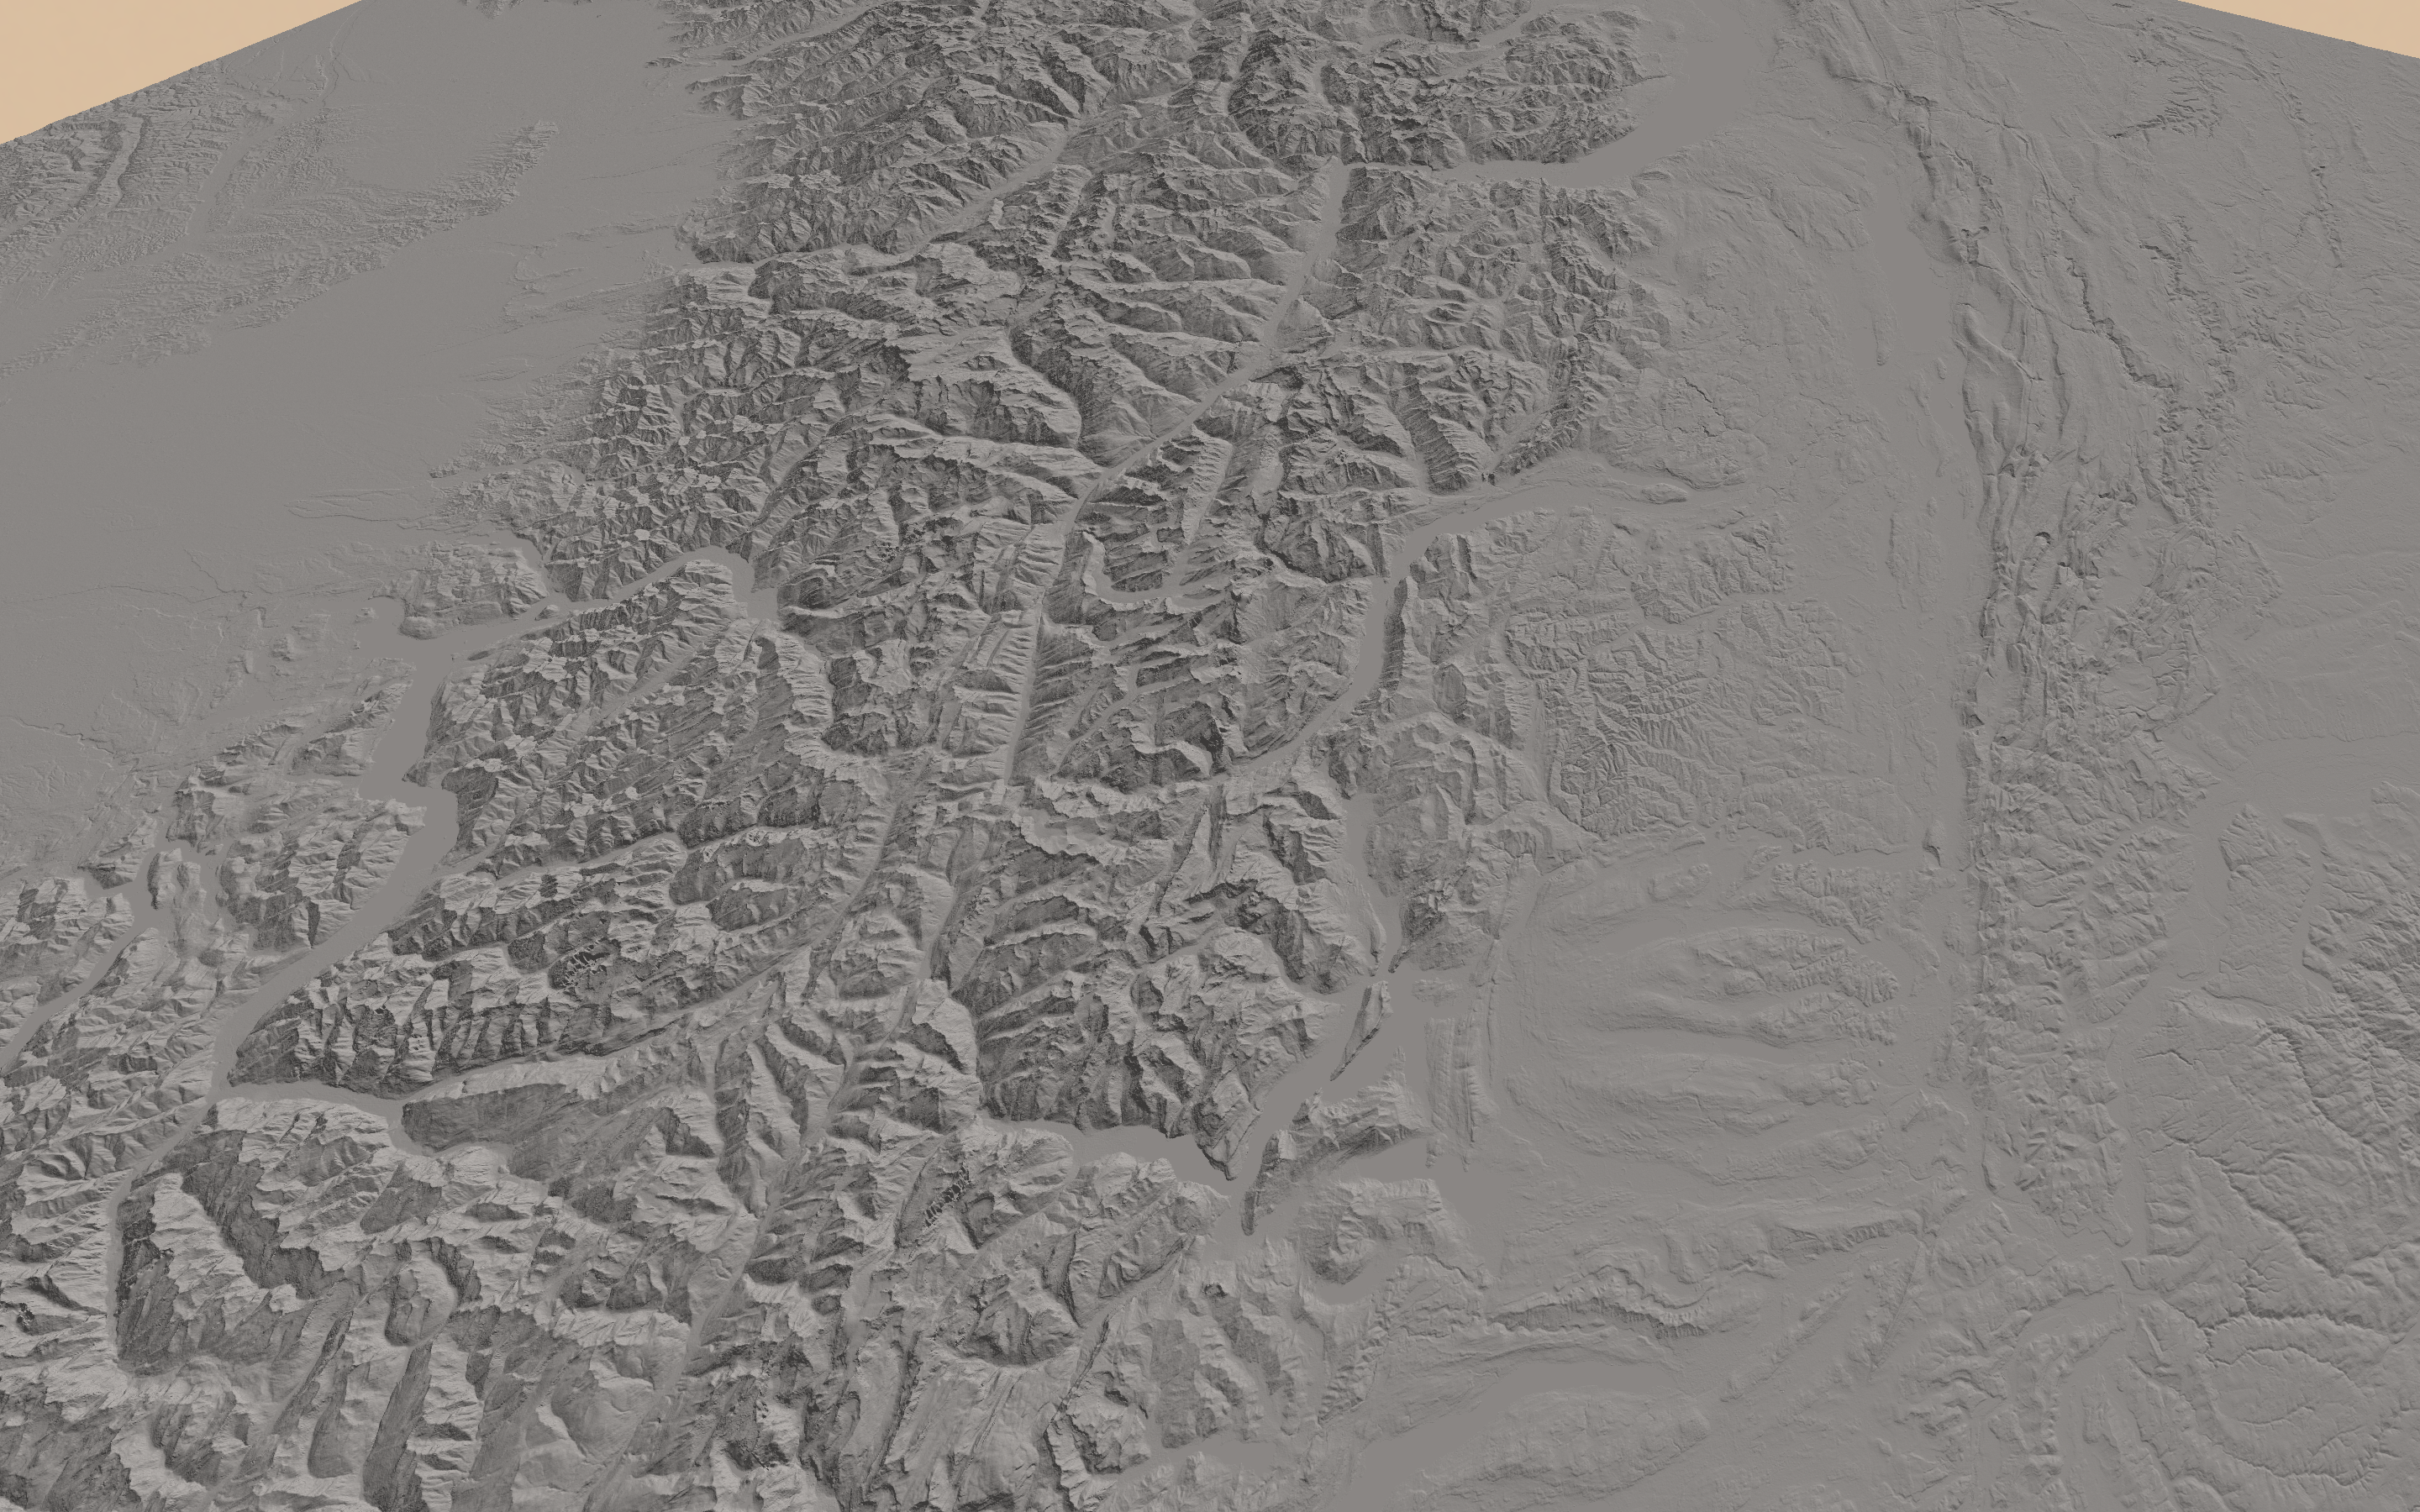
\includegraphics[width=0.4\textwidth]{results-accuracy-large-5-no-lod} }}
  \qquad
  \subfloat[\centering With LOD.]{{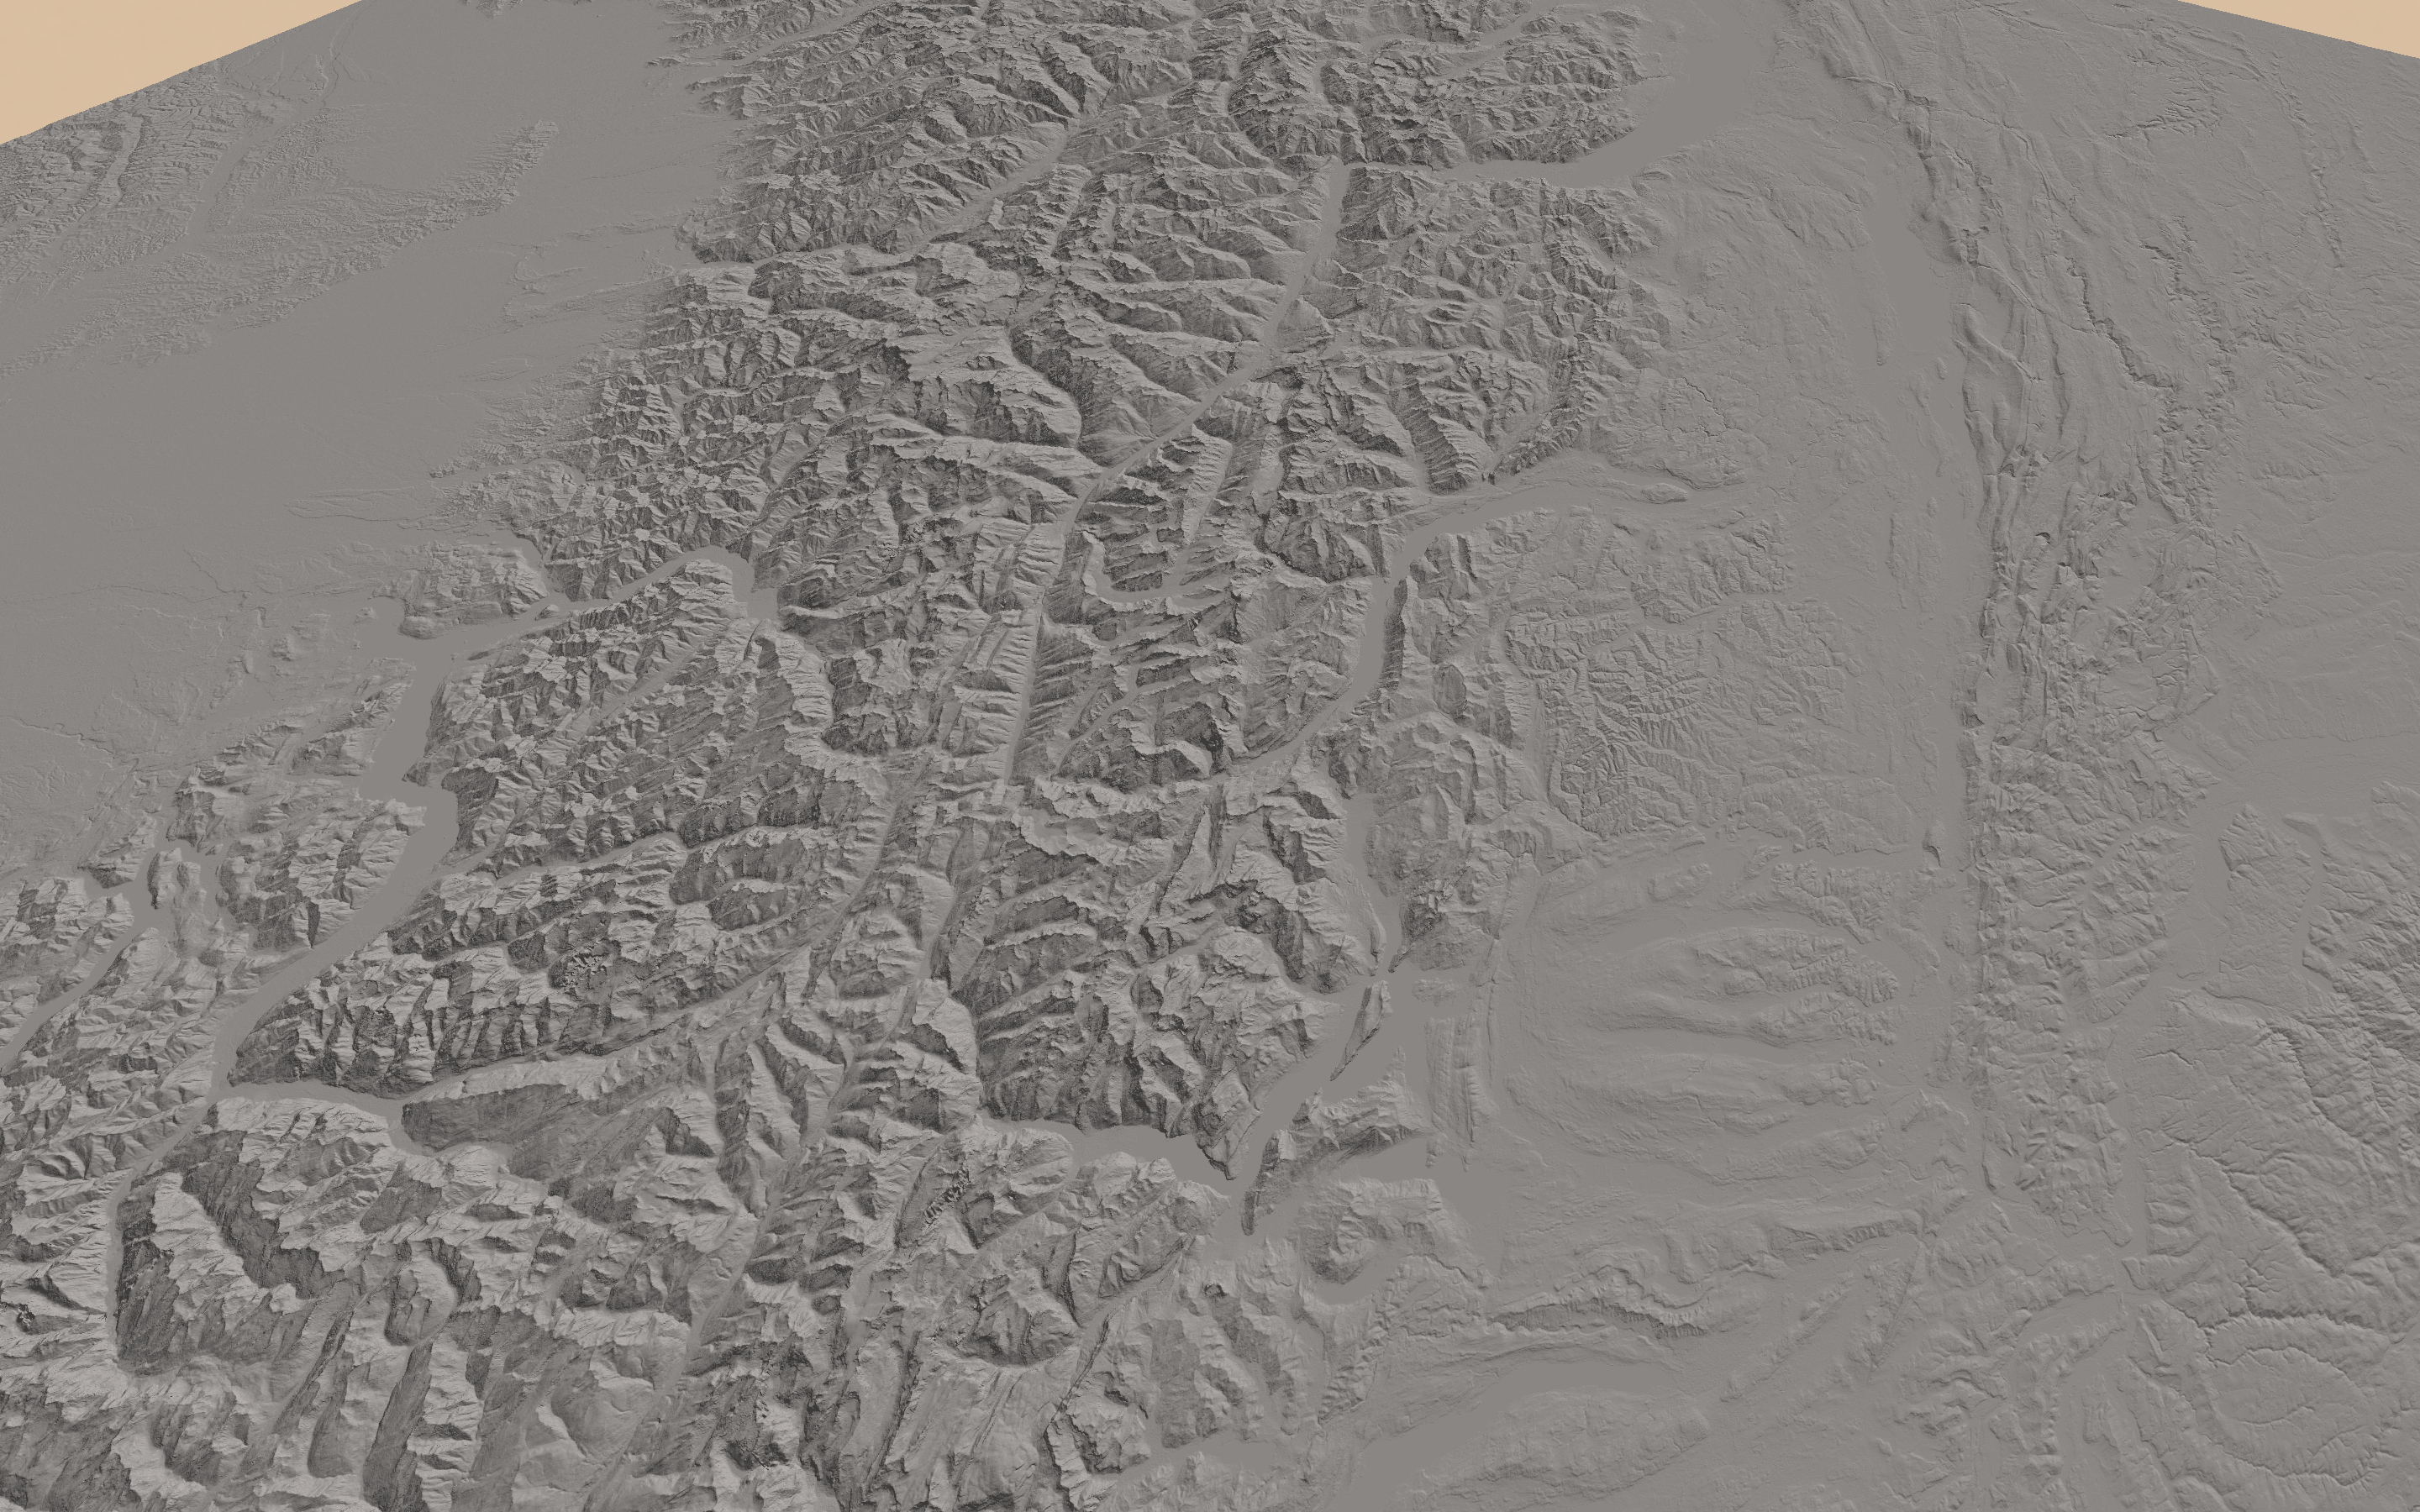
\includegraphics[width=0.4\textwidth]{results-accuracy-large-5-lod} }}
  \qquad
  \subfloat[\centering Absolute difference.]{{
\includegraphics[width=0.4\textwidth]{results-accuracy-large-5-diff} }}
  \qquad
  \subfloat[\centering Absolute difference (binarised).]{{\includegraphics[width=0.4\textwidth]{results-accuracy-large-5-diff-bin} }}
  \caption{Screenshot showcasing the screenshot of a large section of the terrain with no LOD (a), with LOD (b),
   the absolute difference (c) between (a) and (b), and the binarised absolute difference (d) of (c). The computed RMSE is 2.32.}\label{fig:results-large-5}
\end{figure}

\subsubsection{Low FOV Screenshot 1}
\begin{figure}[H]
  \centering
  \subfloat[\centering No LOD.]{{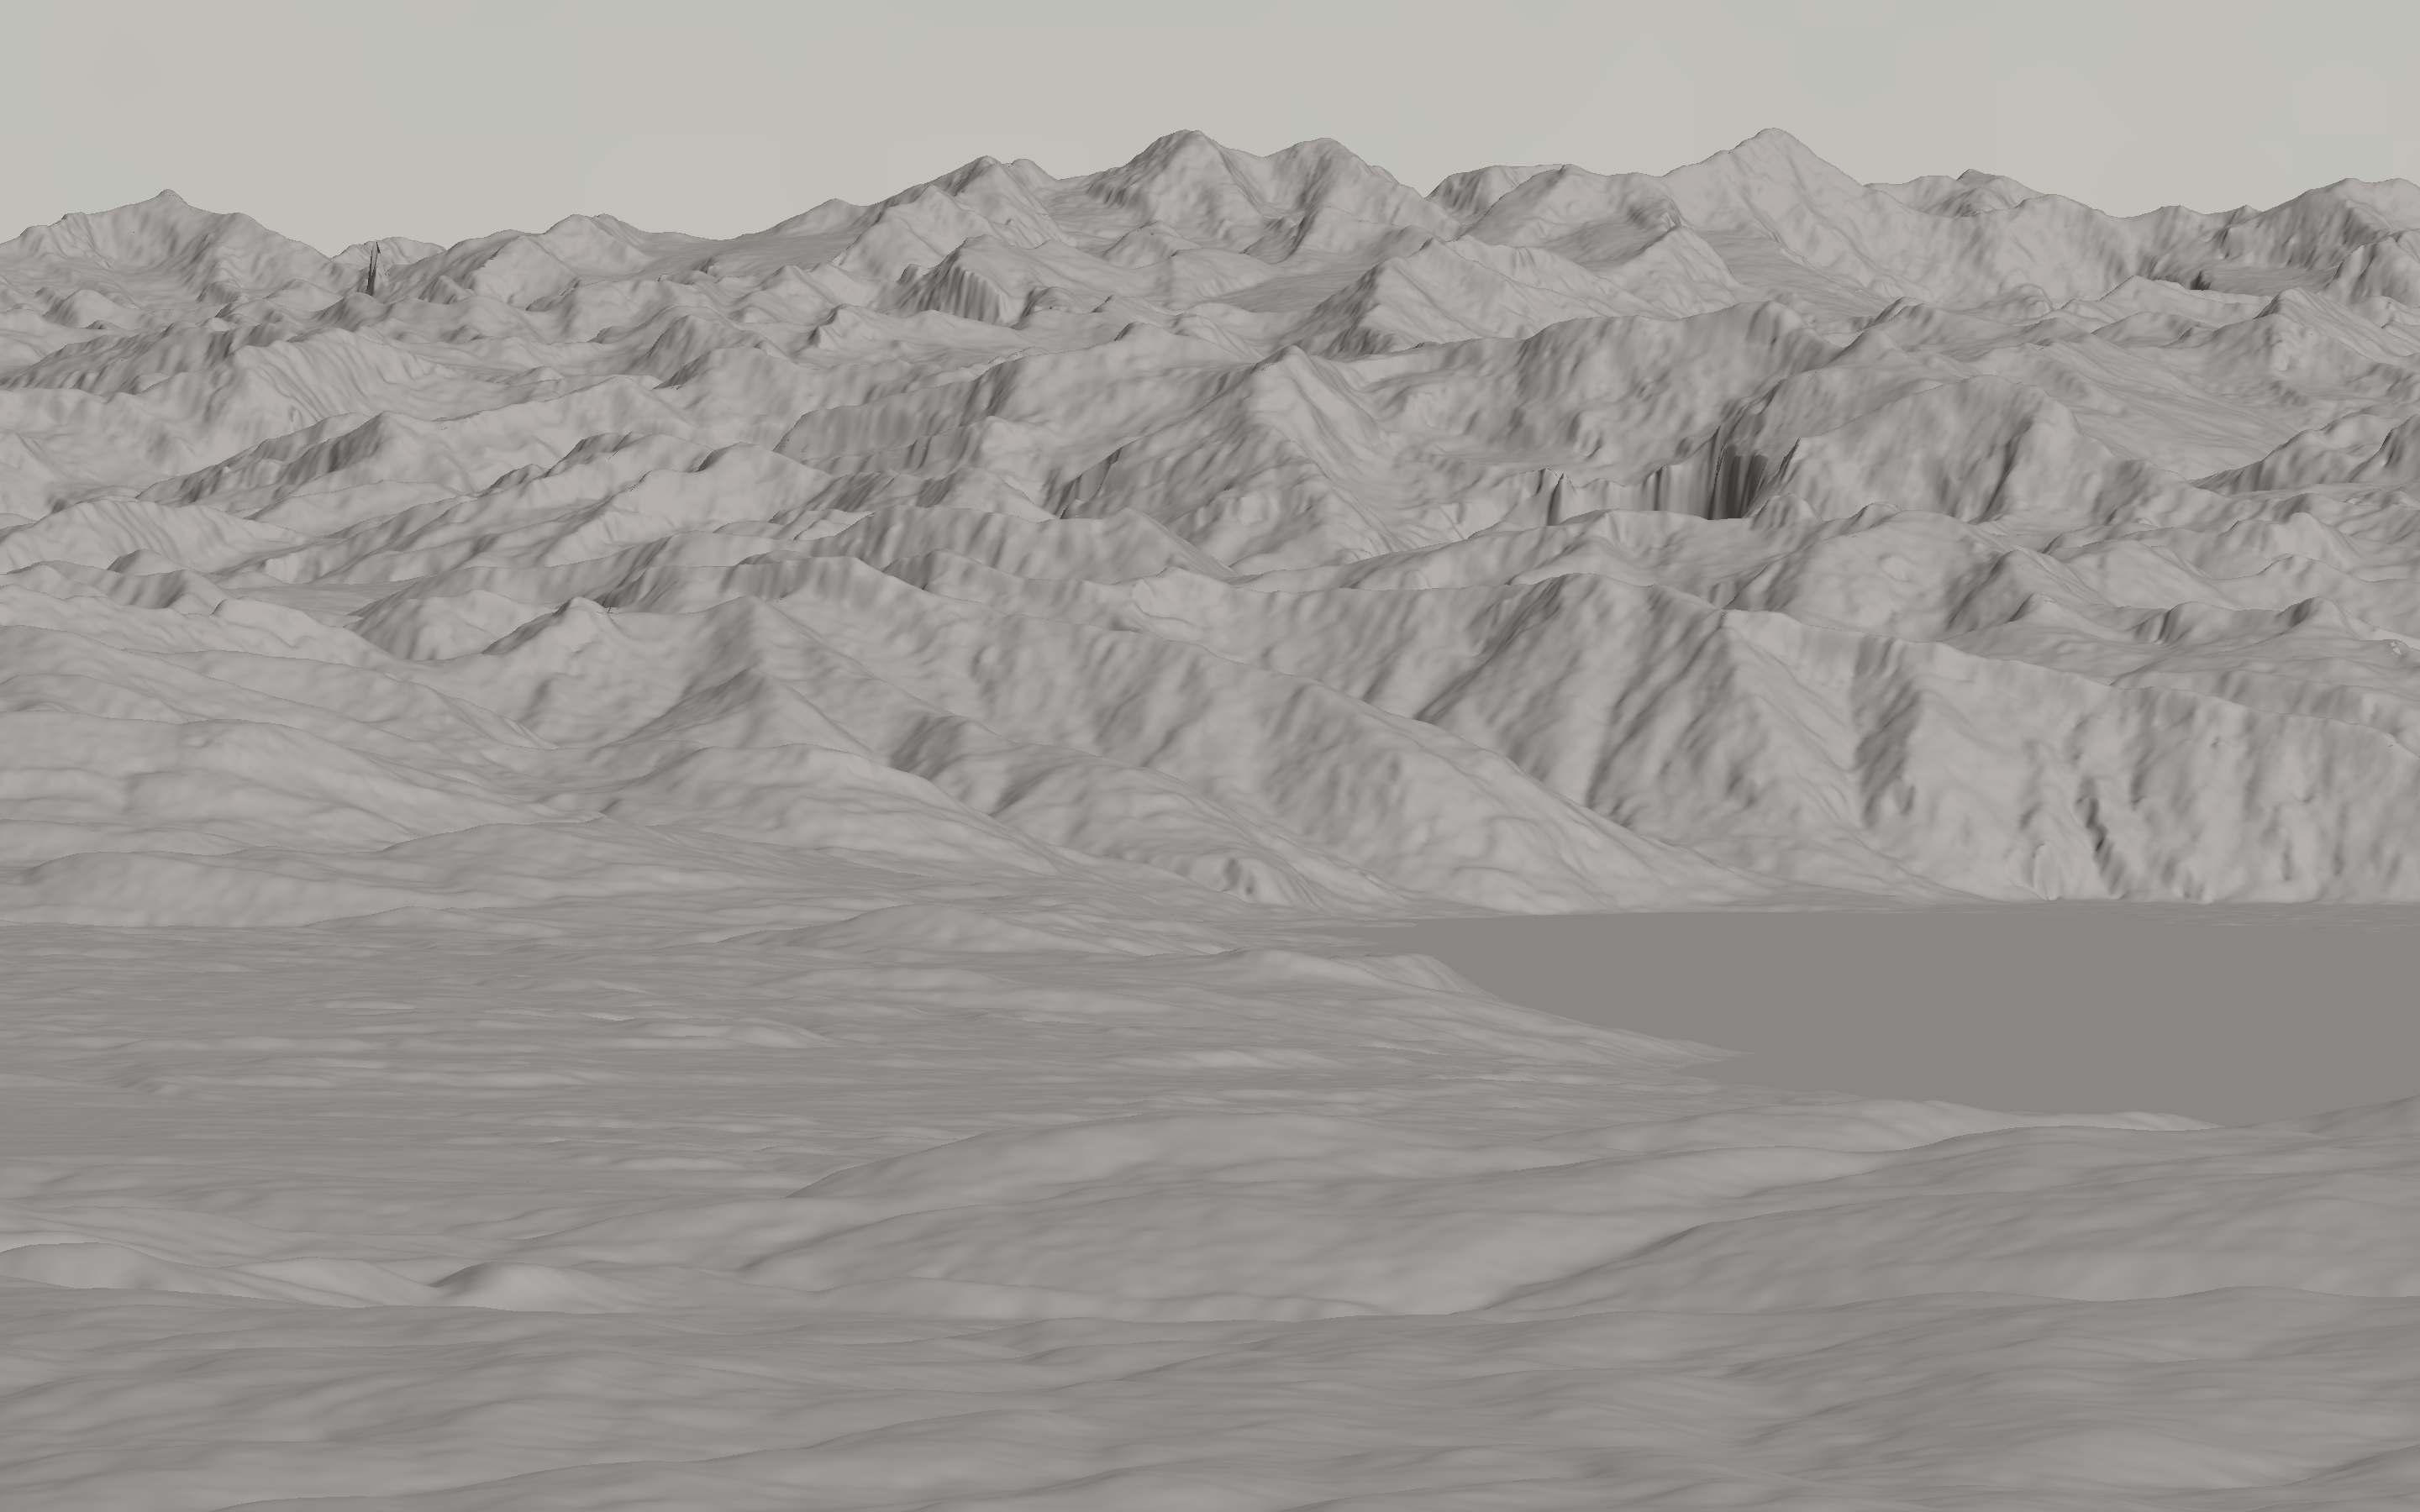
\includegraphics[width=0.4\textwidth]{results-accuracy-zoom-1-no-lod} }}
  \qquad
  \subfloat[\centering With LOD.]{{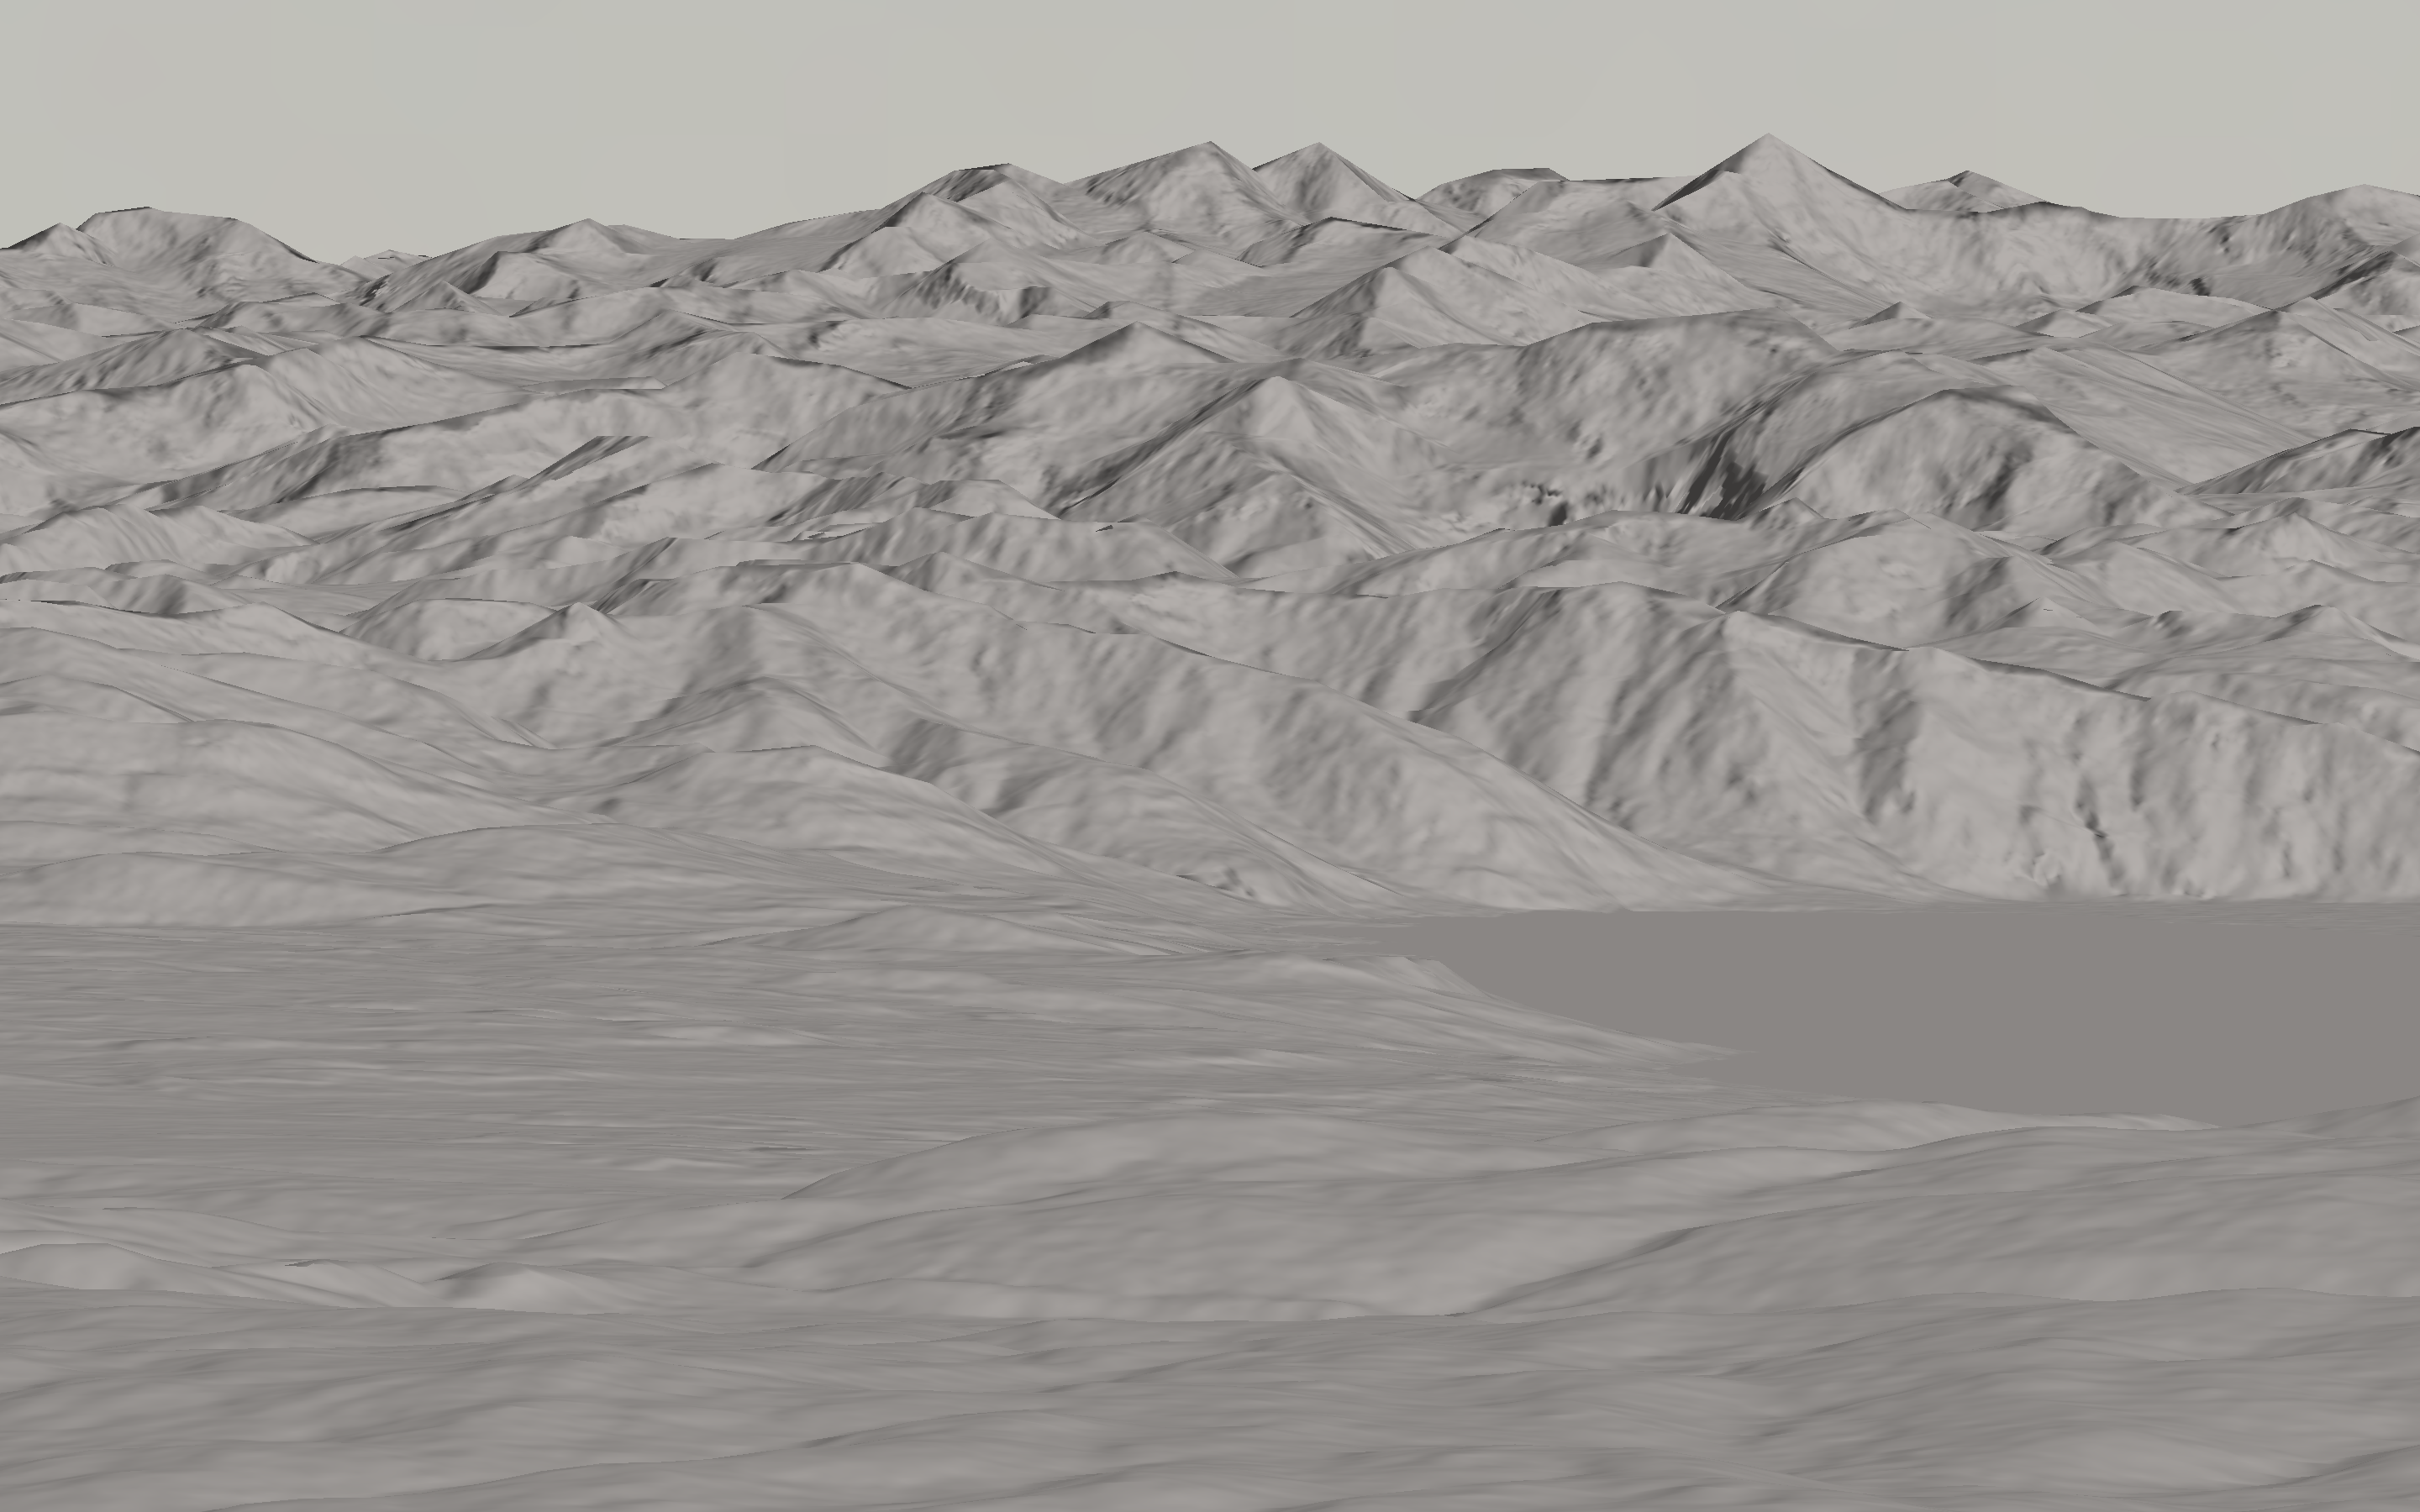
\includegraphics[width=0.4\textwidth]{results-accuracy-zoom-1-lod} }}
  \qquad
  \subfloat[\centering Absolute difference.]{{\includegraphics[width=0.4\textwidth]{results-accuracy-zoom-1-diff} }}
  \qquad
  \subfloat[\centering Absolute difference (binarised).]{{\includegraphics[width=0.4\textwidth]{results-accuracy-zoom-1-diff-bin} }}
  \caption{Screenshot showcasing the screenshot of a small section of the terrain with no LOD (a), with LOD (b),
  the absolute difference (c) between (a) and (b) and the binarised absolute difference (d) of (c). The FOV is set to $6^{\circ}$ and the computed RSME is 4.82.}\label{fig:results-zoom-1}
\end{figure}
\subsubsection{Low FOV Screenshot 2}
\begin{figure}[H]
  \centering
  \subfloat[\centering No LOD.]{{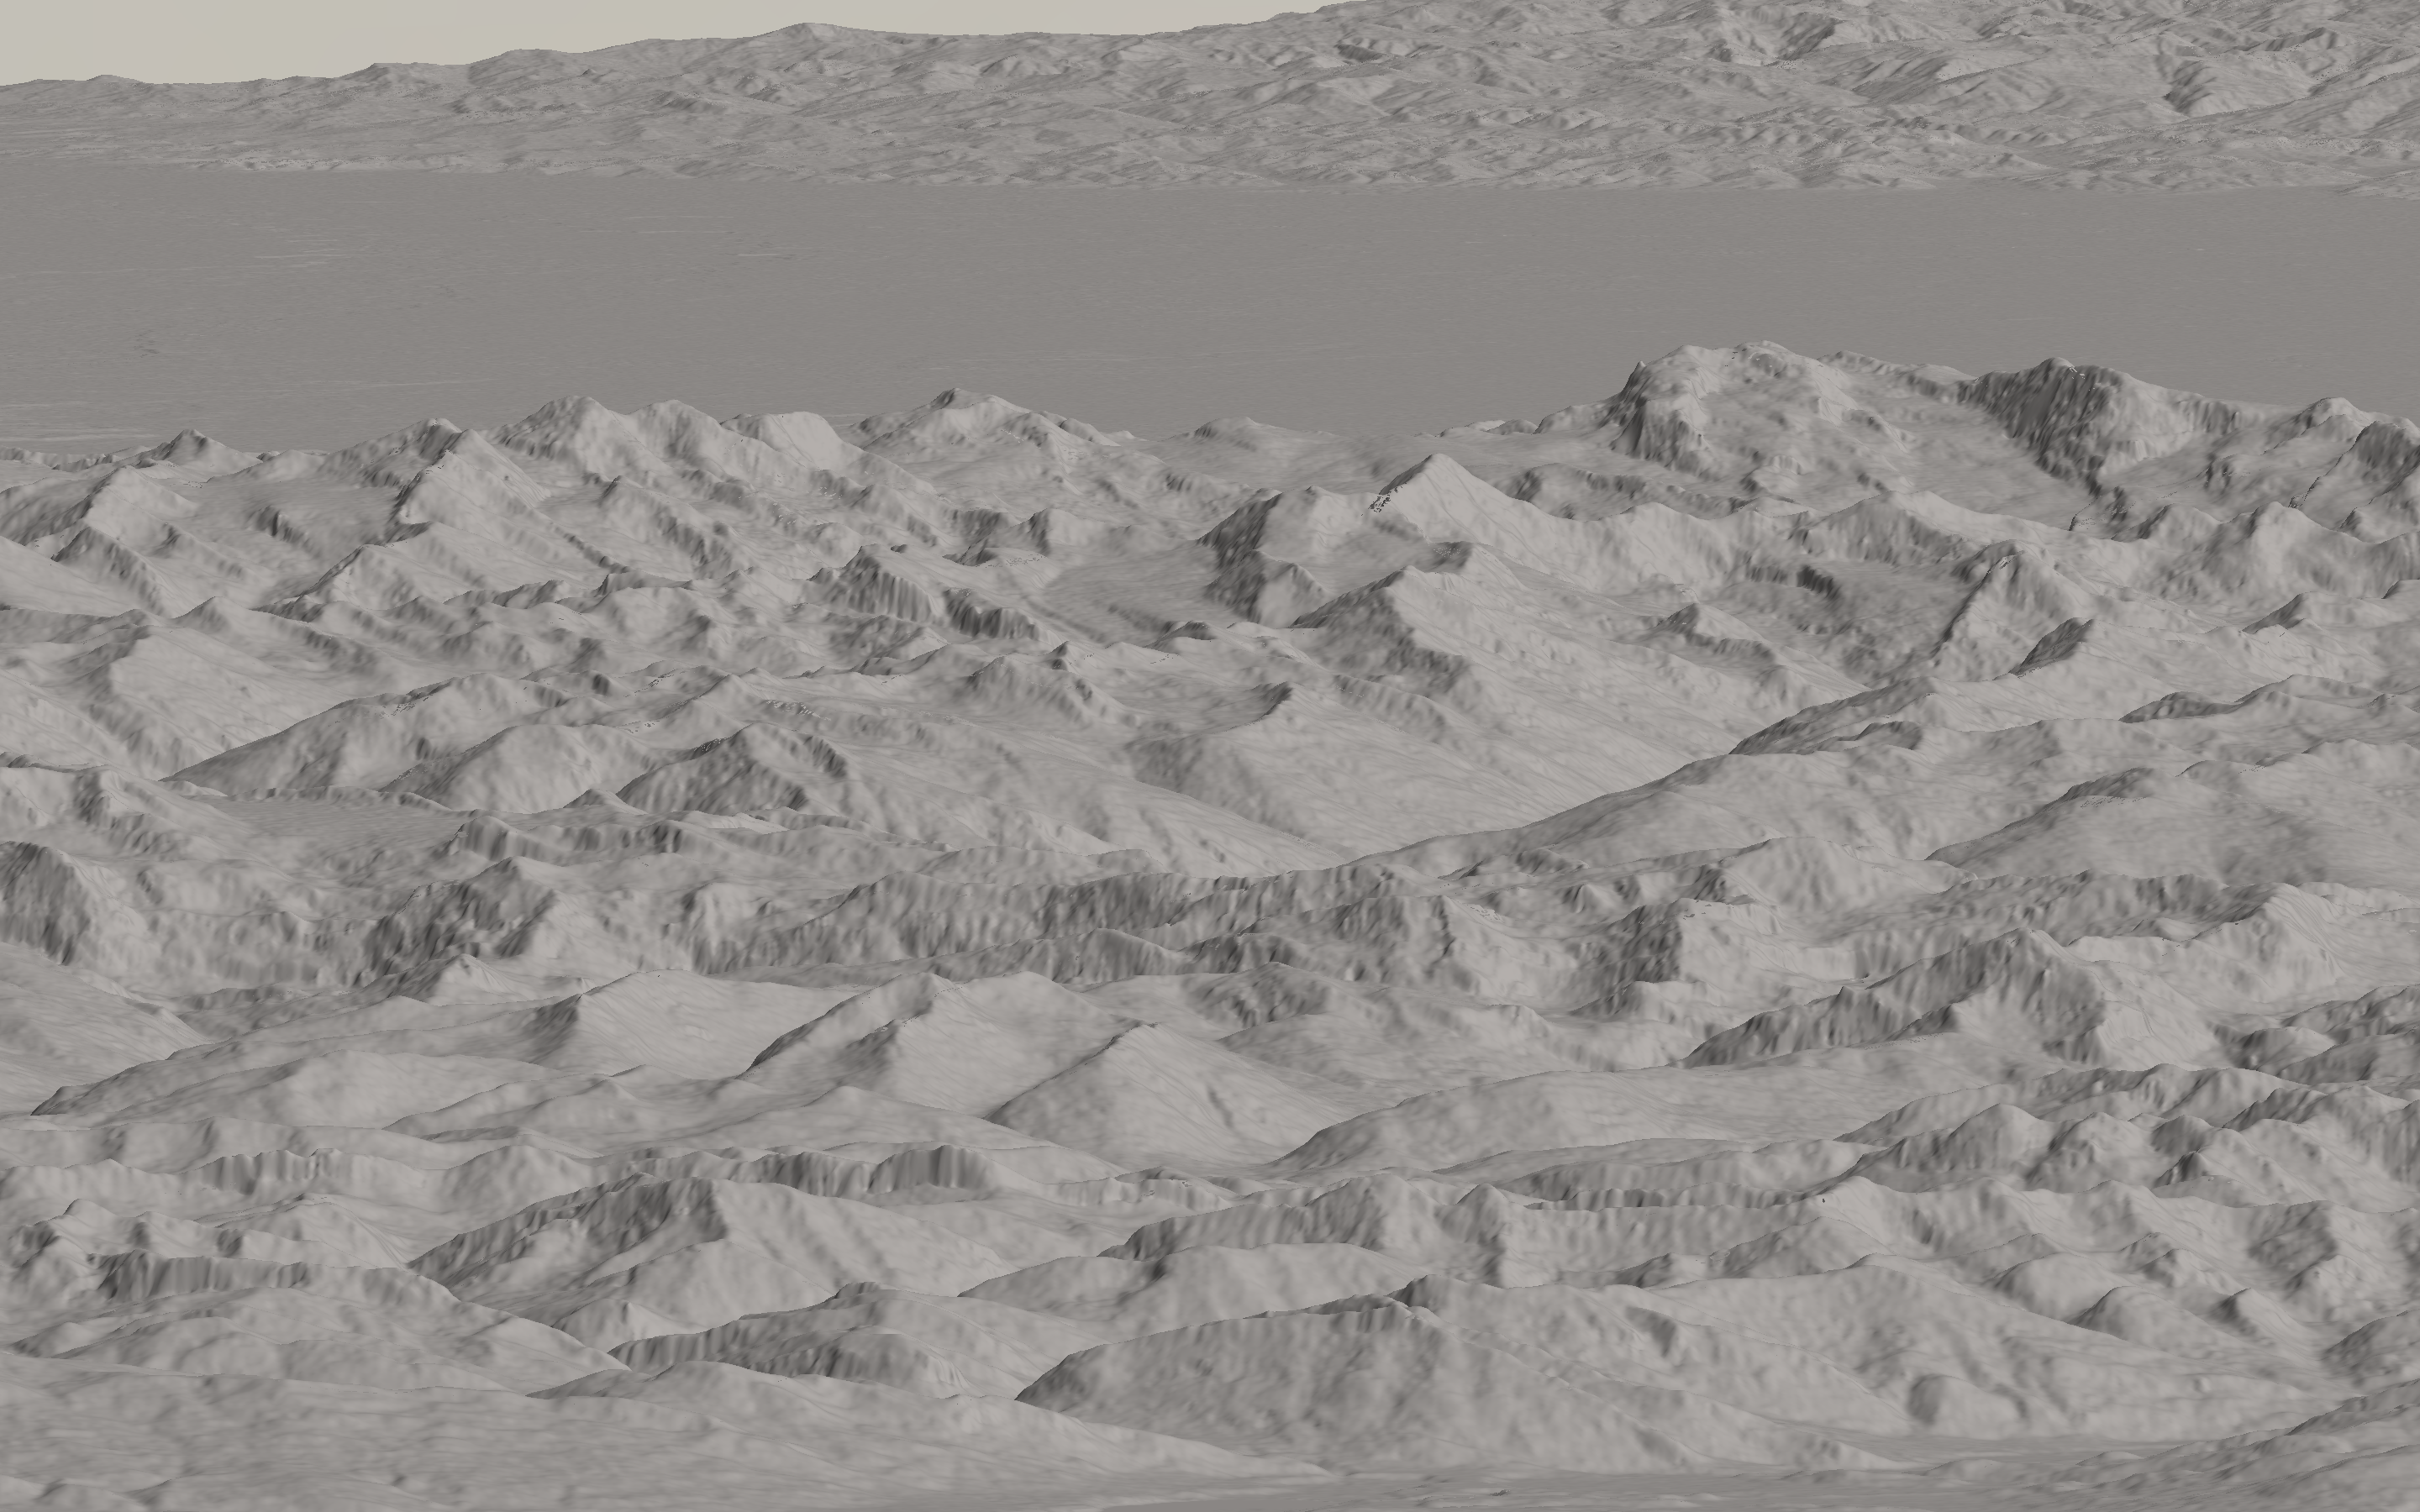
\includegraphics[width=0.4\textwidth]{results-accuracy-zoom-2-no-lod} }}
  \qquad
  \subfloat[\centering With LOD.]{{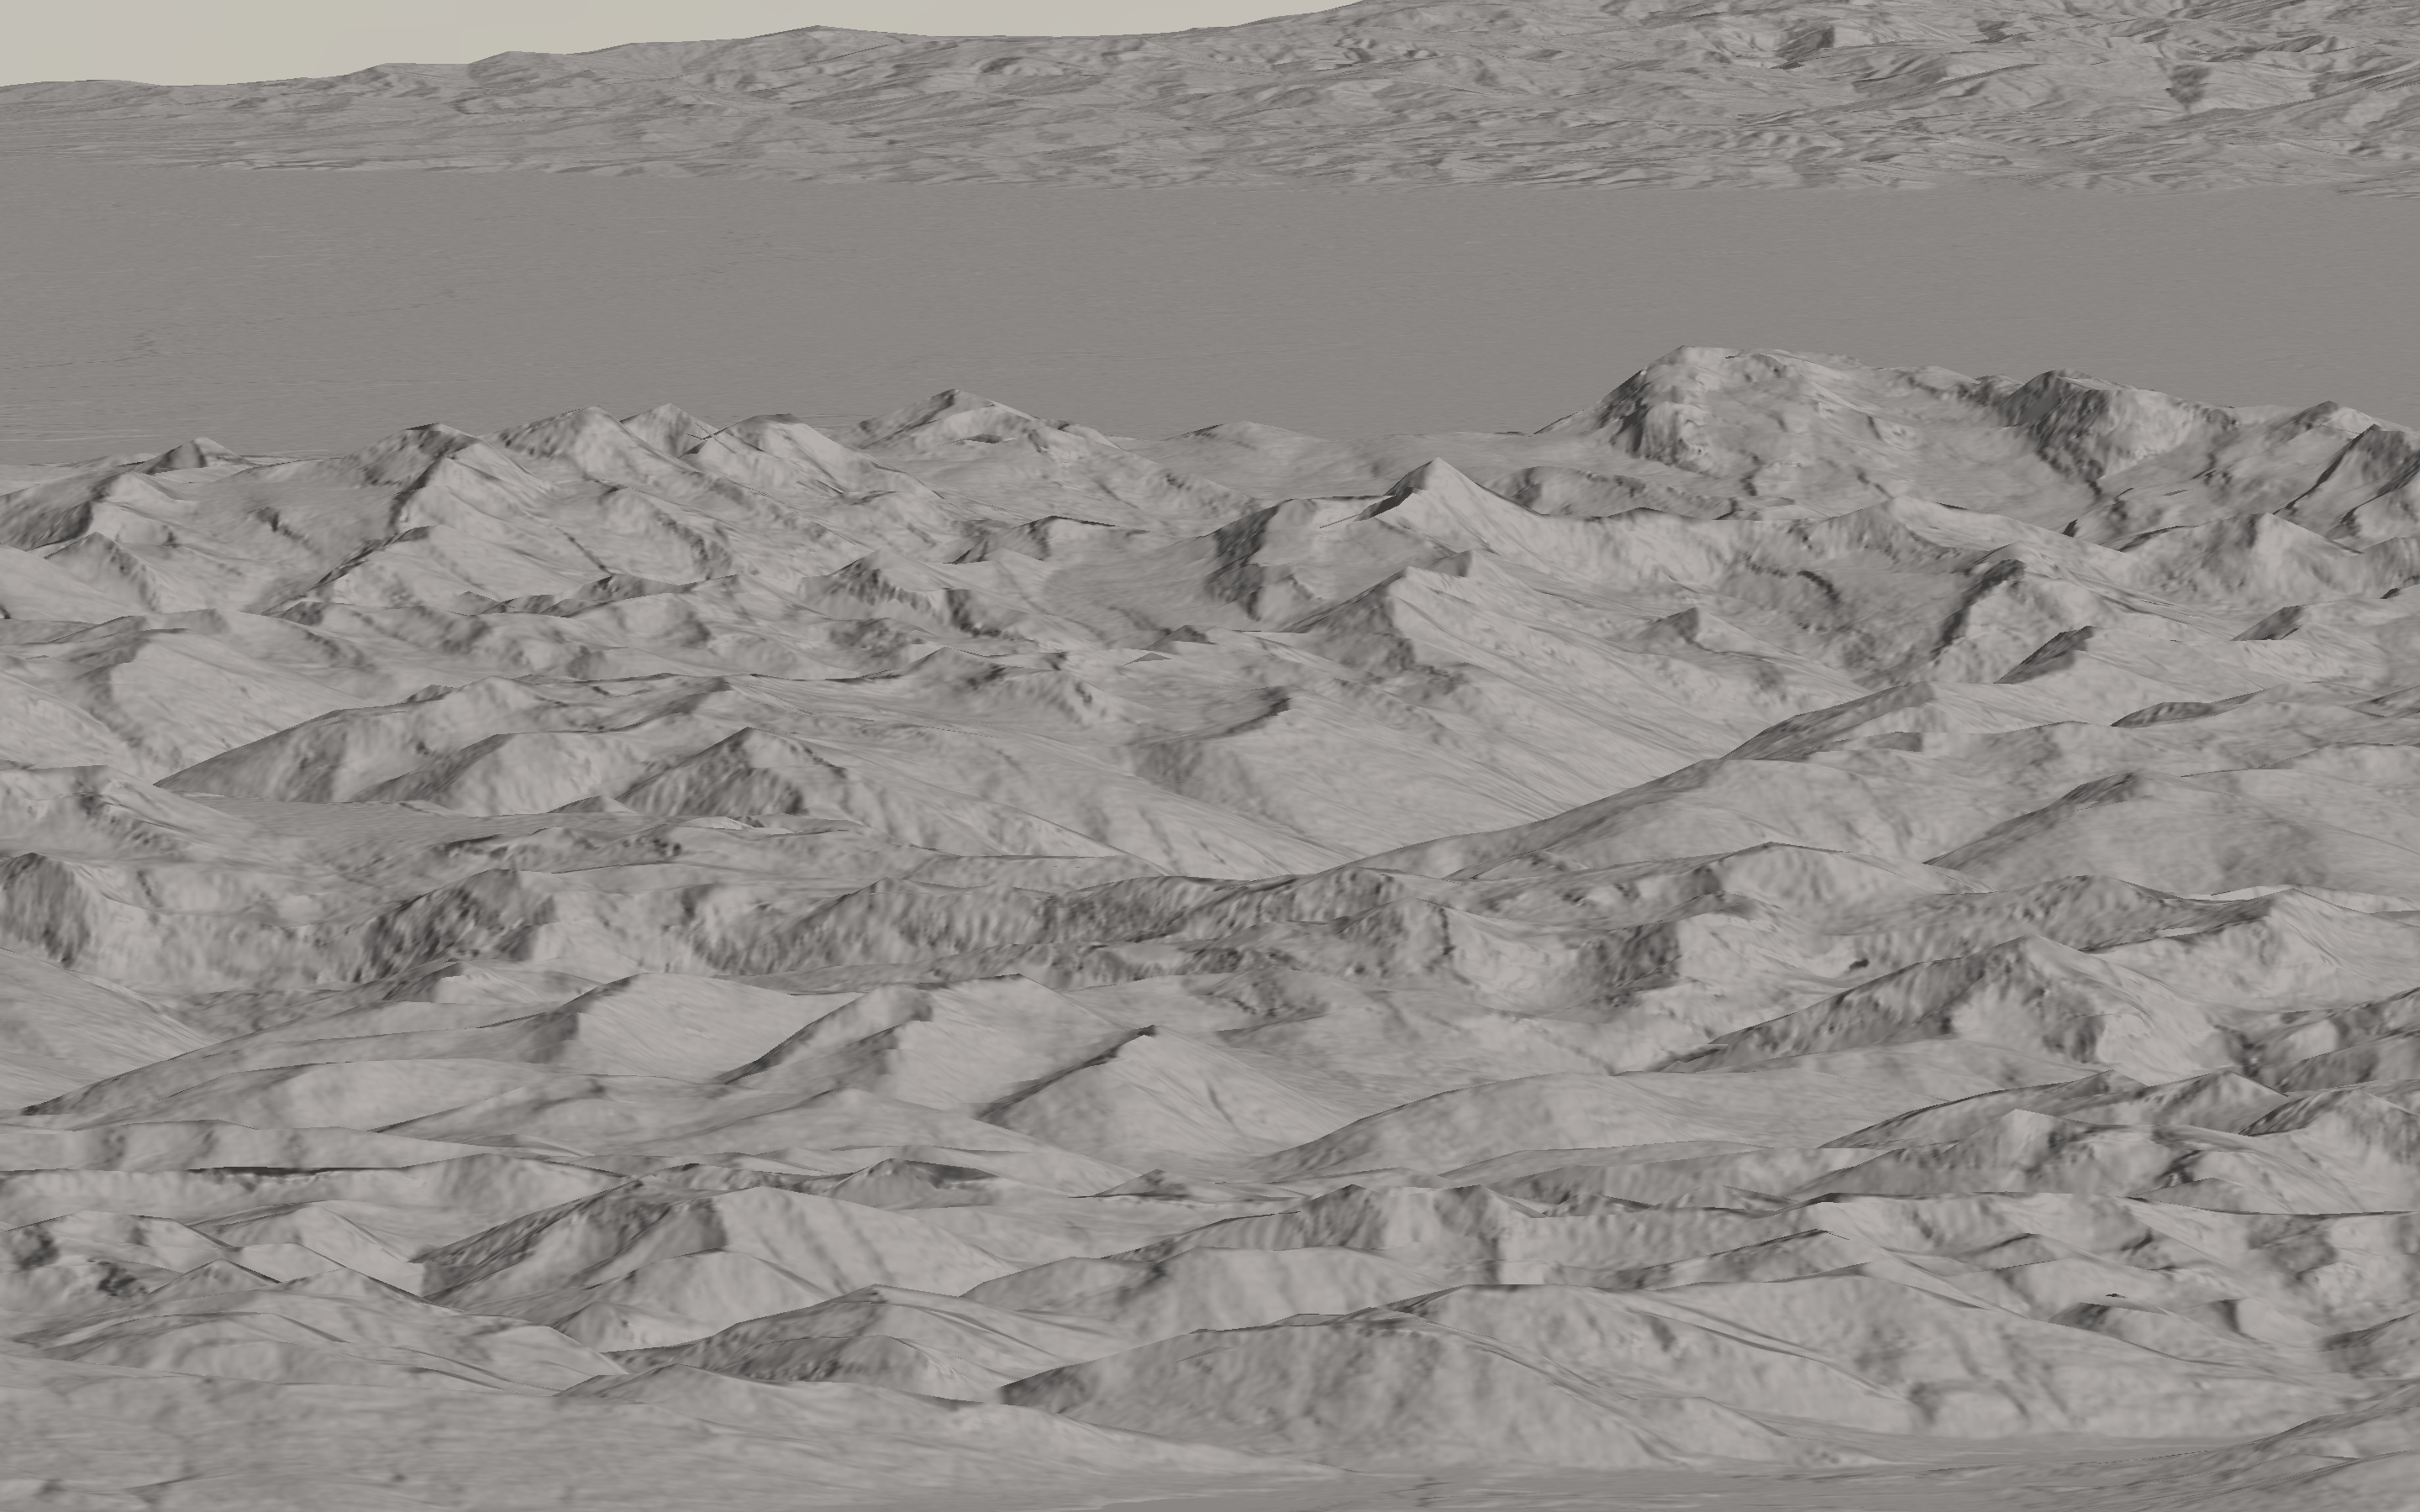
\includegraphics[width=0.4\textwidth]{results-accuracy-zoom-2-lod} }}
  \qquad
  \subfloat[\centering Absolute difference.]{{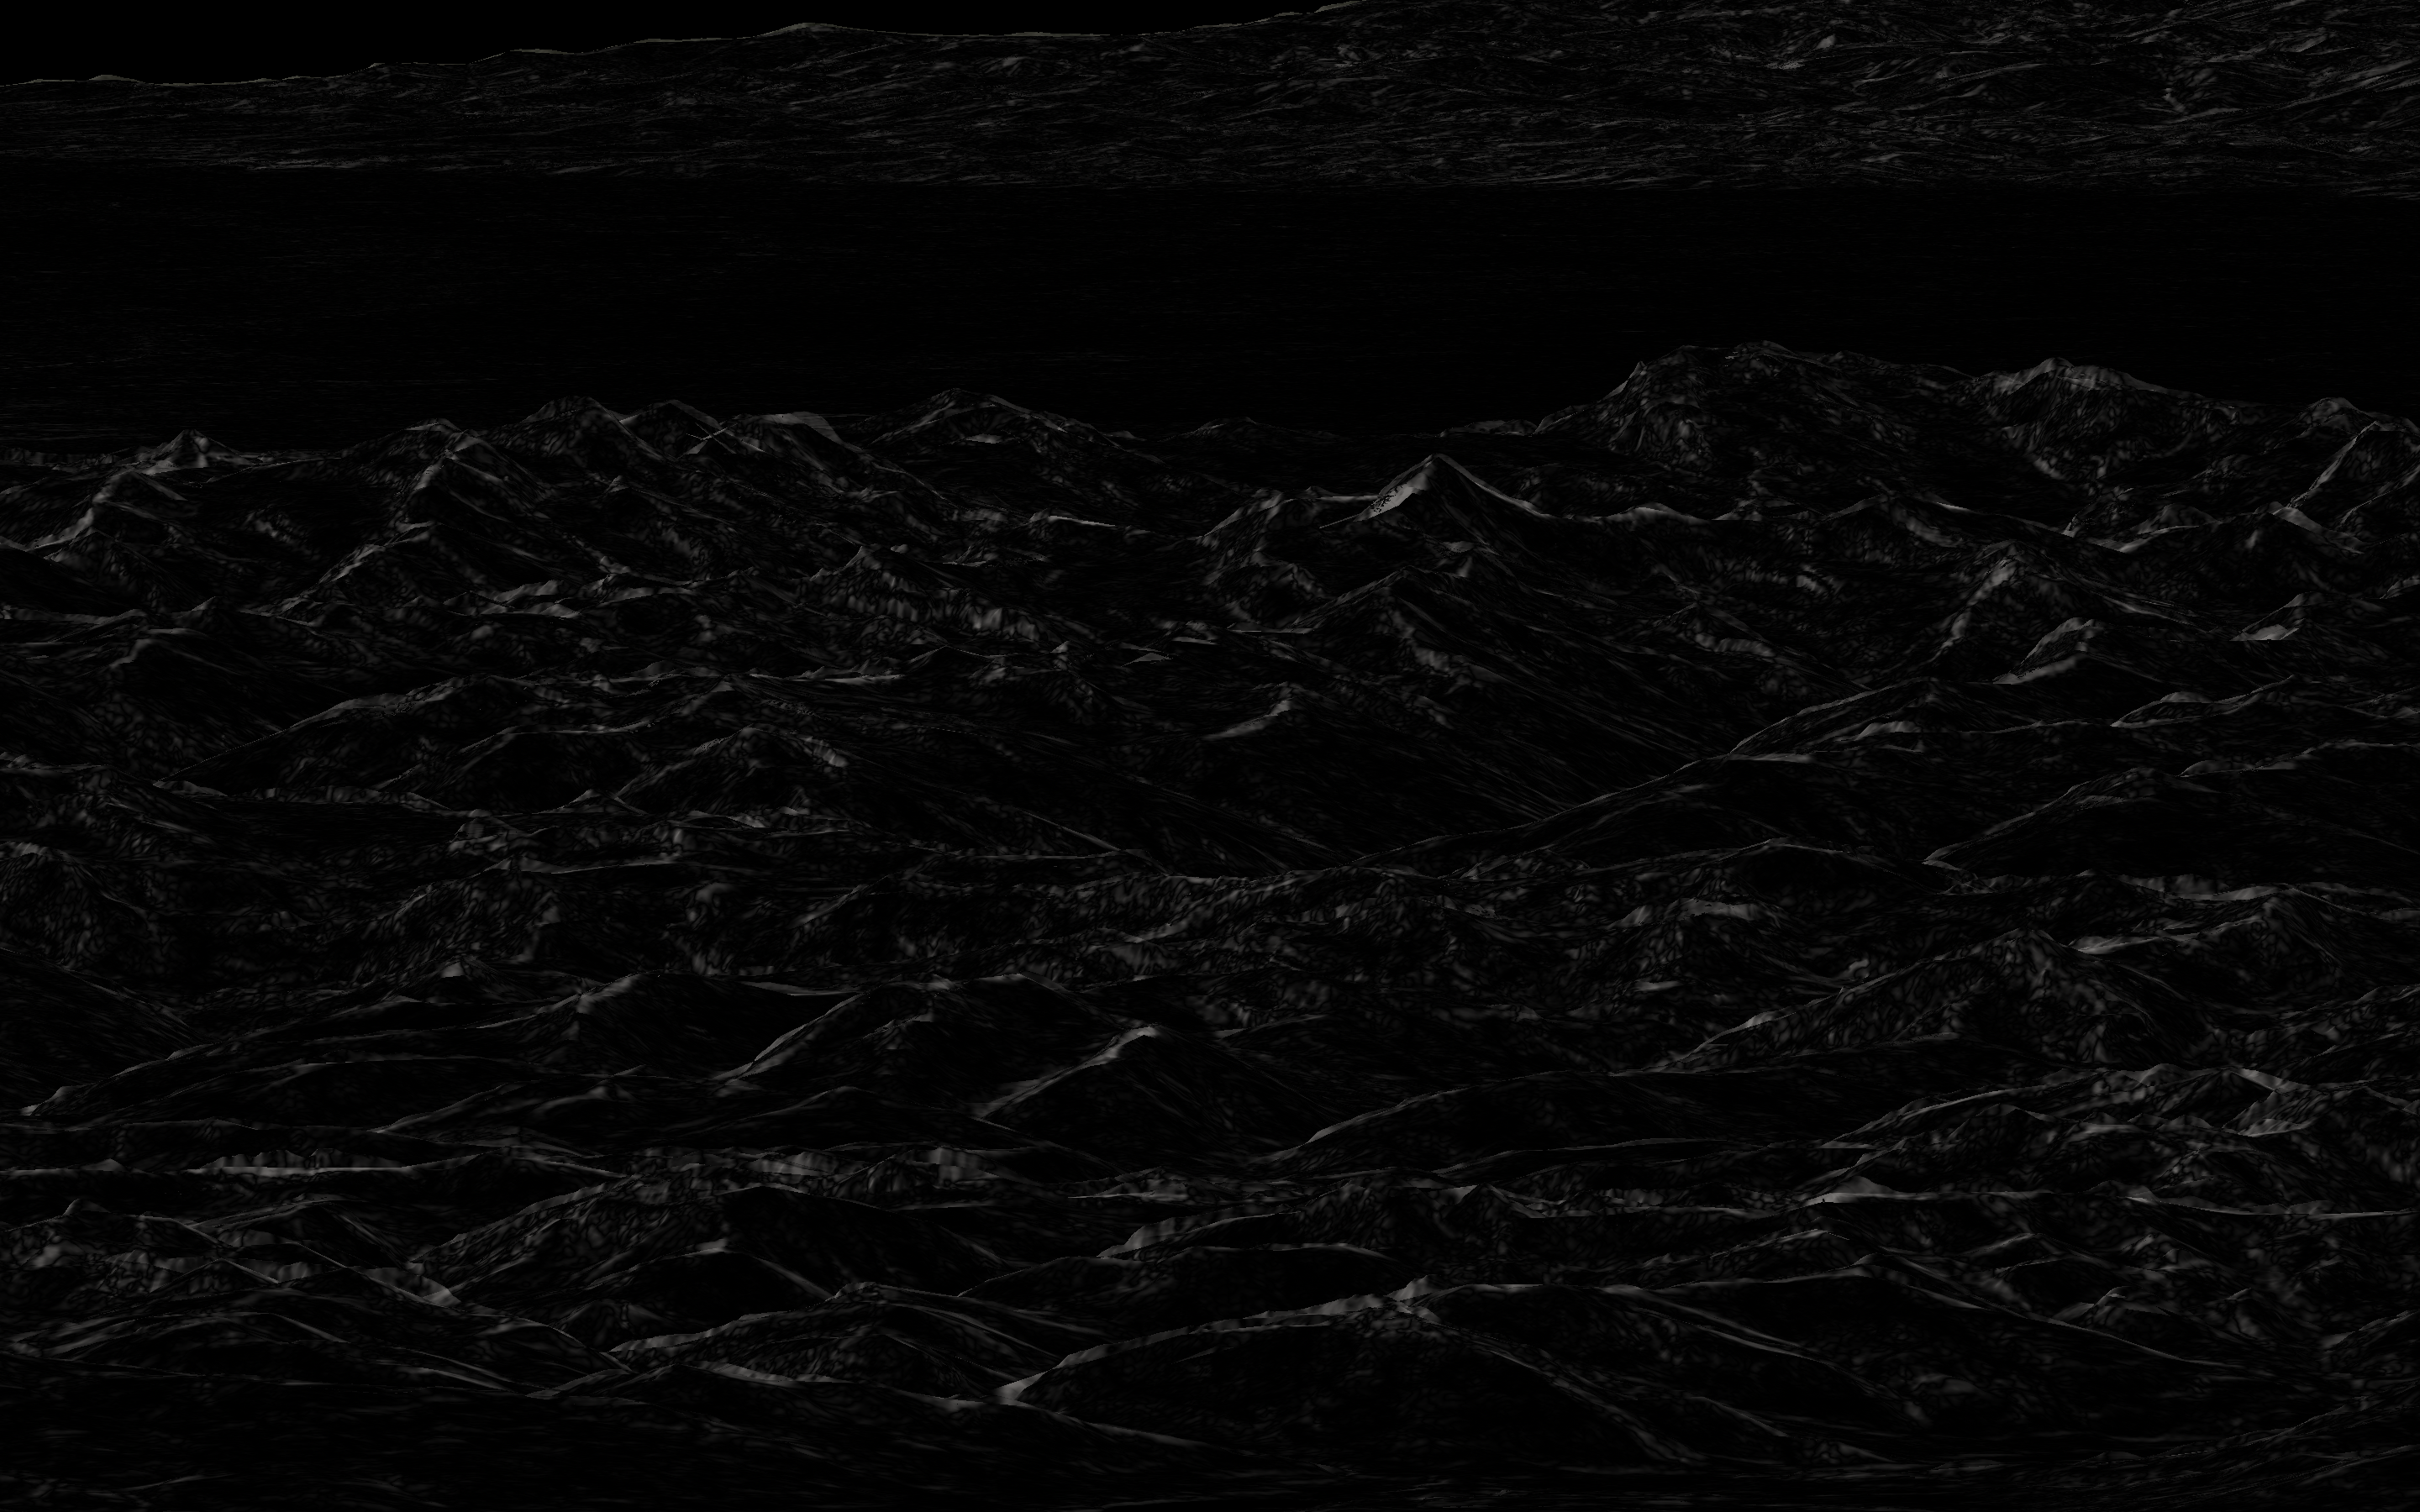
\includegraphics[width=0.4\textwidth]{results-accuracy-zoom-2-diff} }}
  \qquad
  \subfloat[\centering Absolute difference (binarised).]{{\includegraphics[width=0.4\textwidth]{results-accuracy-zoom-2-diff-bin} }}
  \caption{Screenshot showcasing the screenshot of a small section of the terrain with no LOD (a), with LOD (b),
  the absolute difference (c) between (a) and (b) and the binarised absolute difference (d) of (c). The FOV is set to $3^{\circ}$ and the computed RSME is 5.71.}\label{fig:results-zoom-2}
\end{figure}
\subsubsection{Low FOV Screenshot 3}
\begin{figure}[H]
  \centering
  \subfloat[\centering No LOD.]{{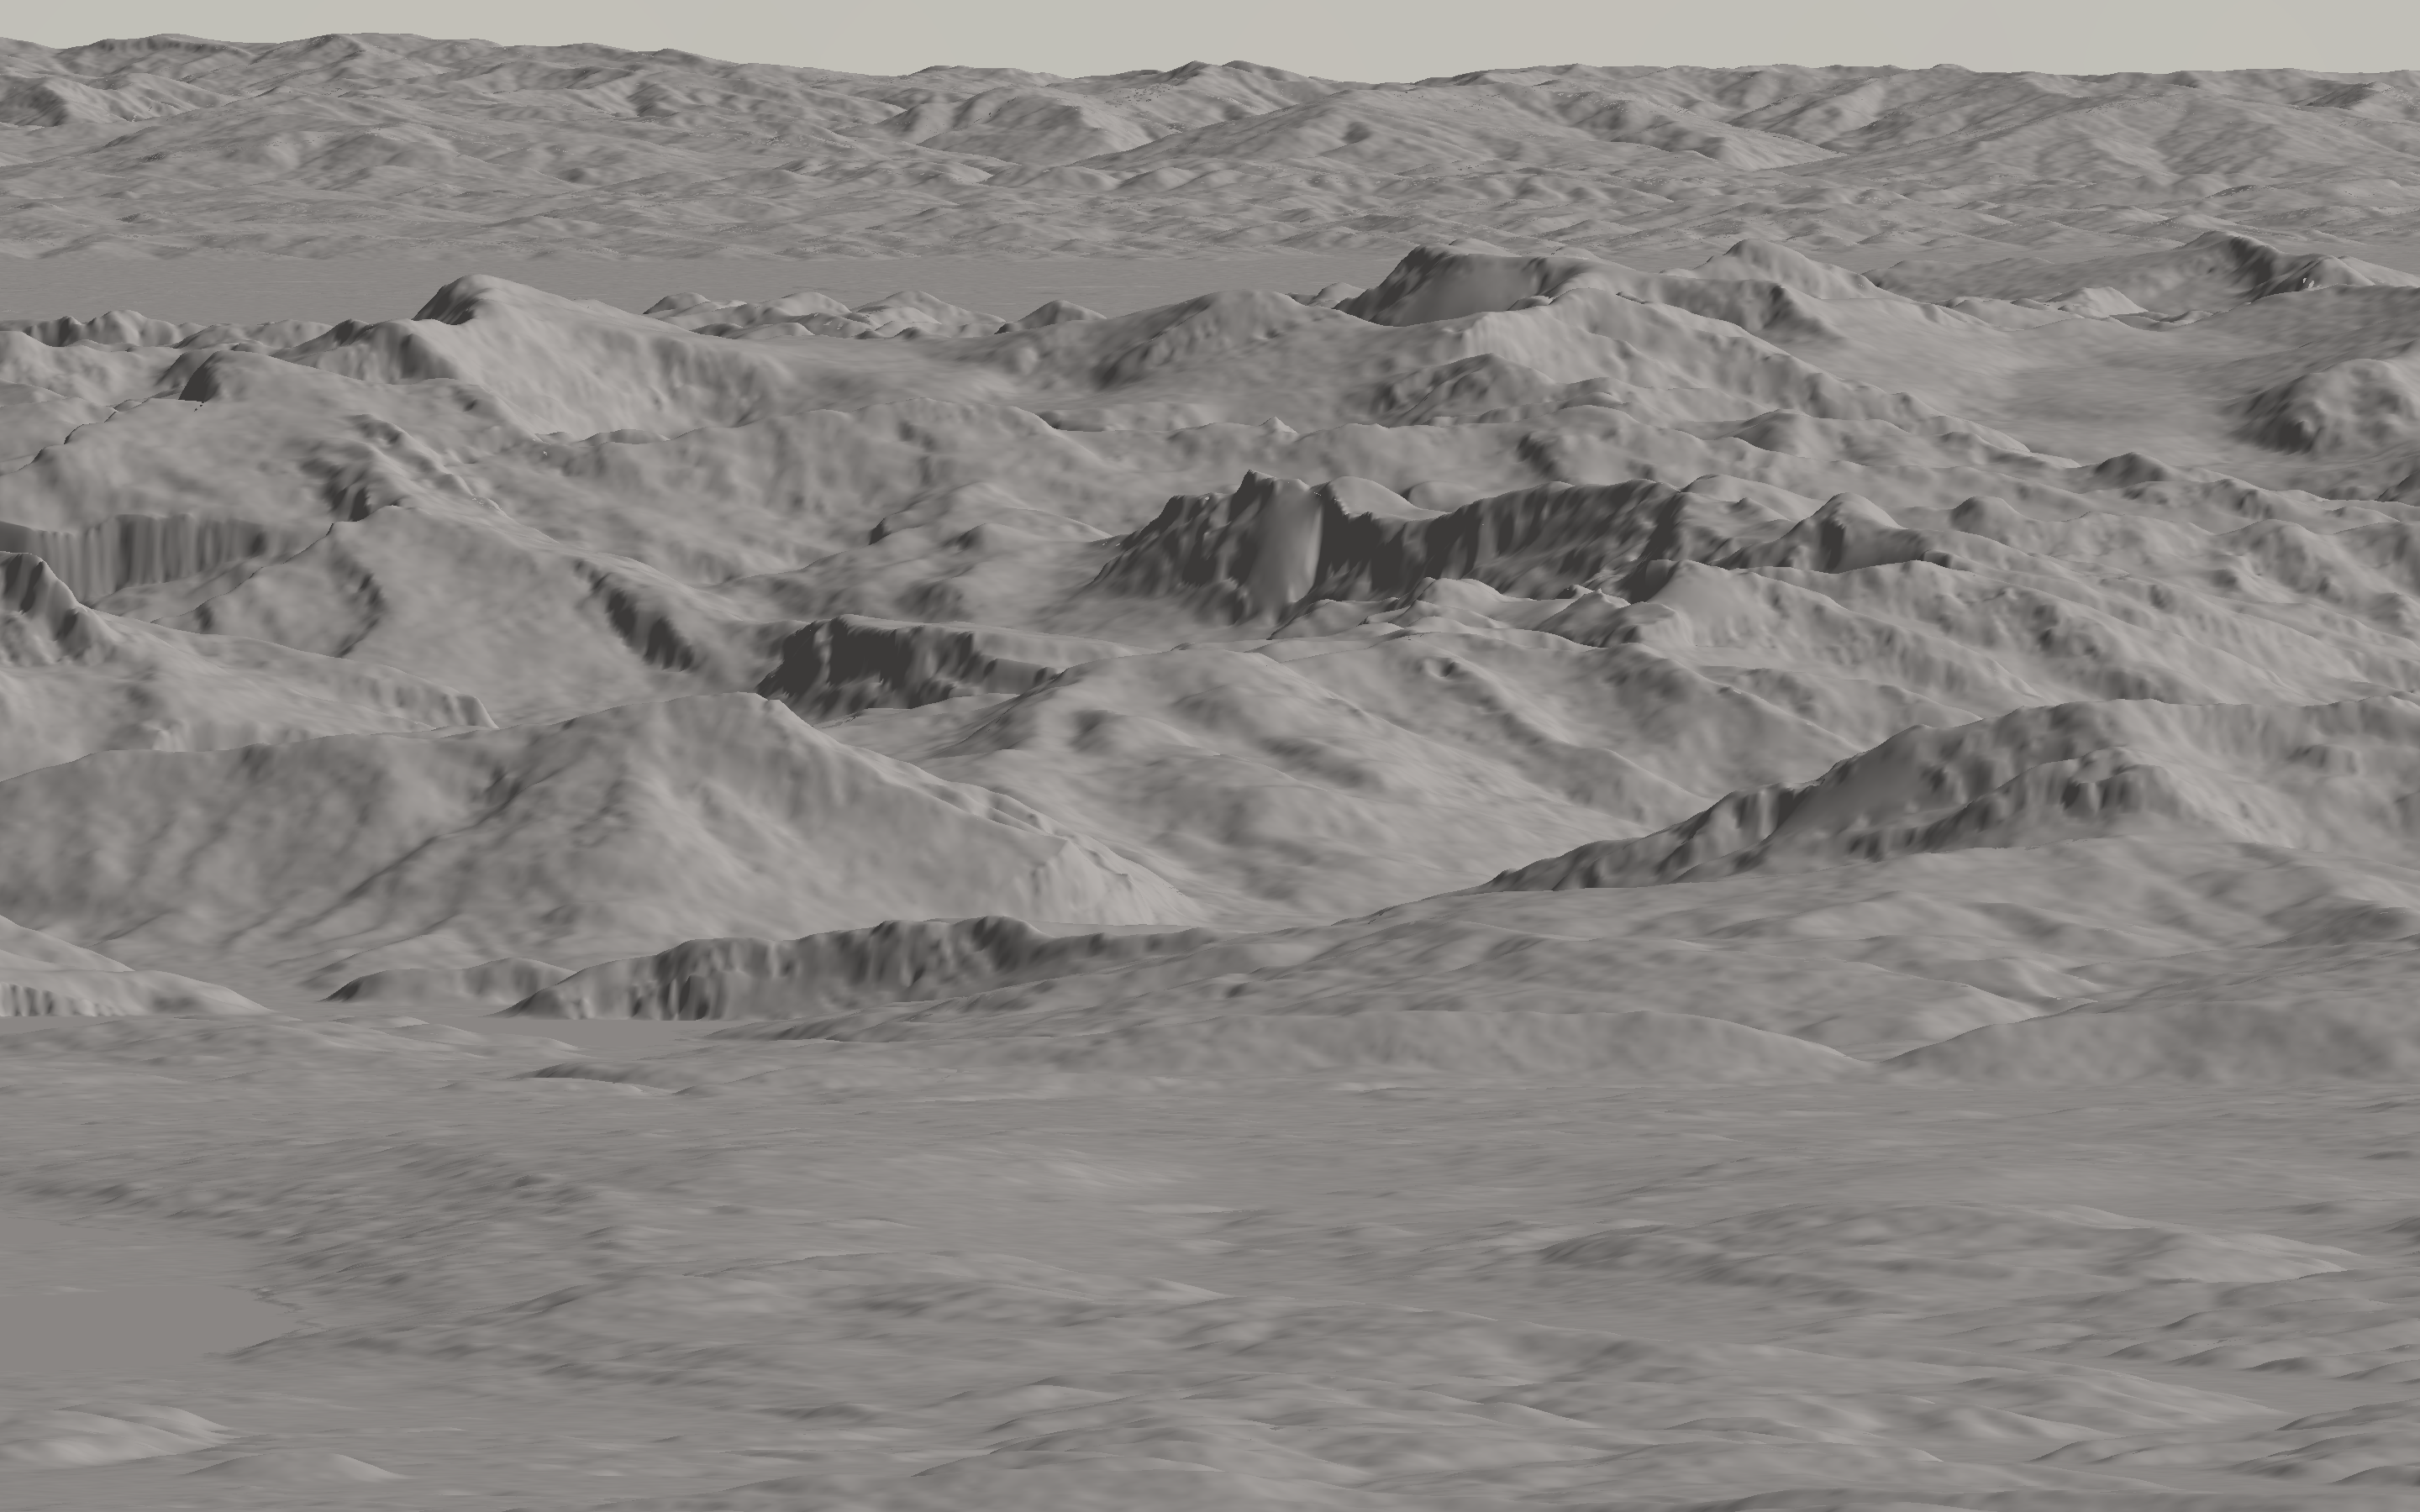
\includegraphics[width=0.4\textwidth]{results-accuracy-zoom-3-no-lod} }}
  \qquad
  \subfloat[\centering With LOD.]{{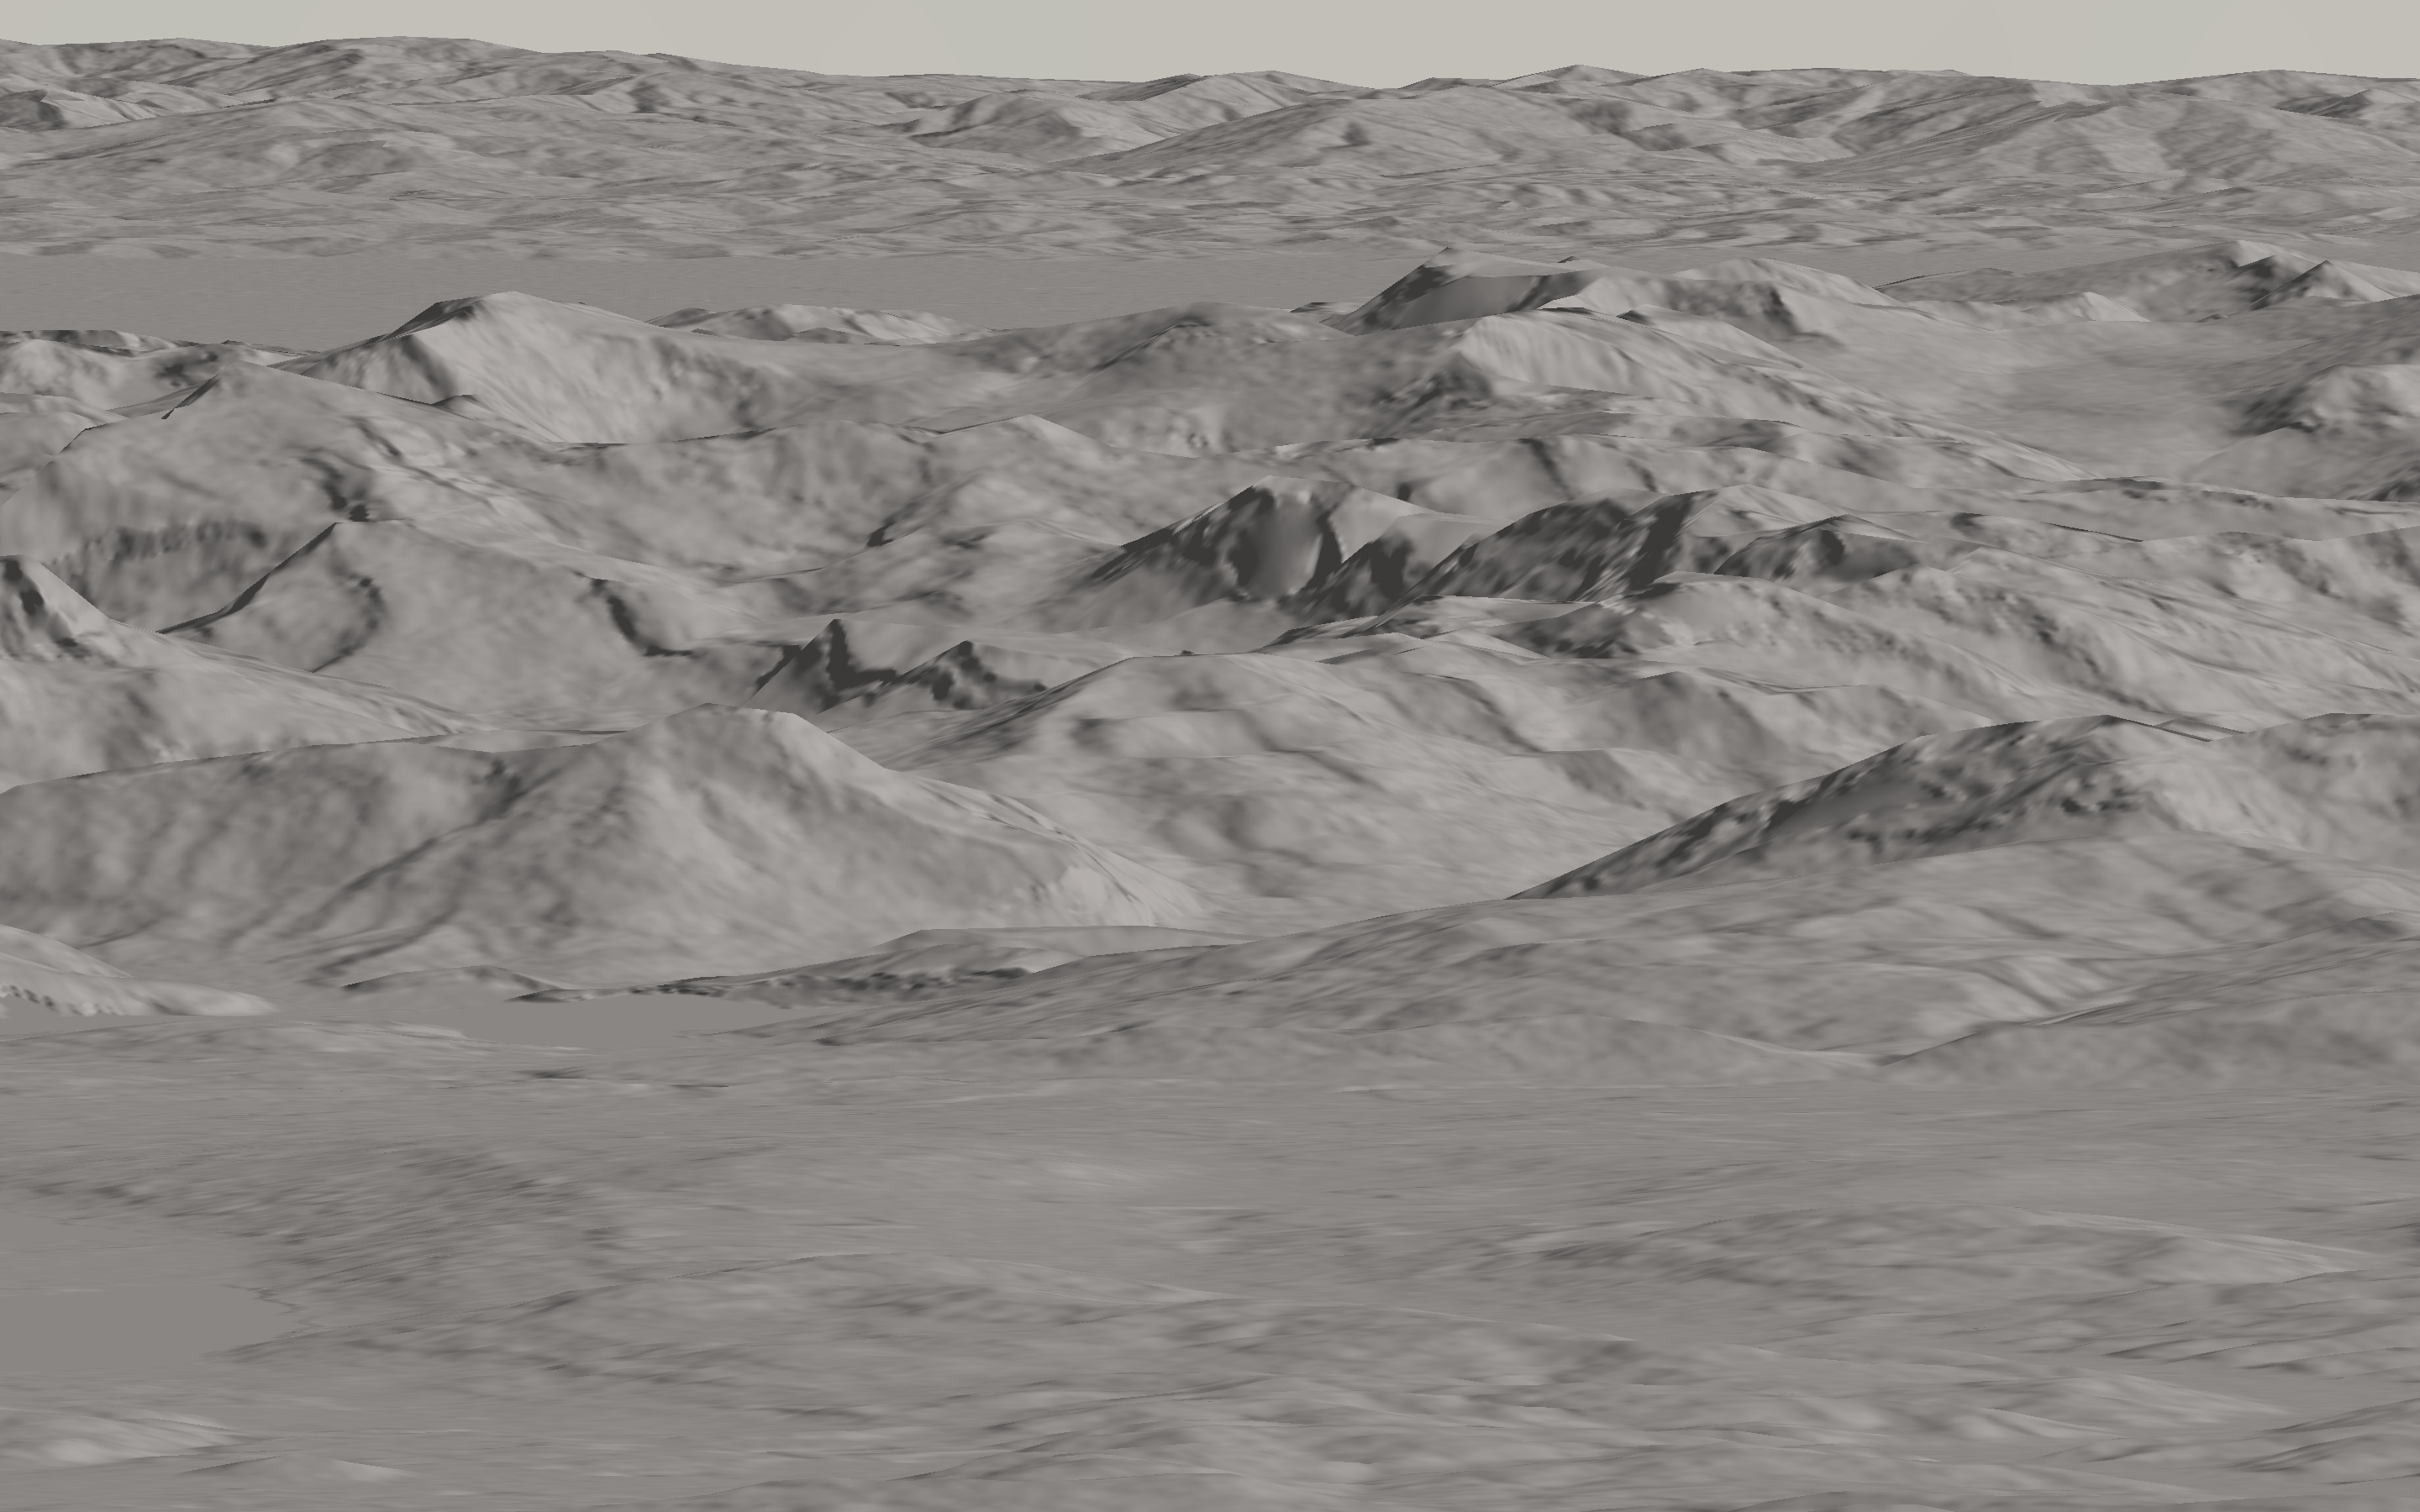
\includegraphics[width=0.4\textwidth]{results-accuracy-zoom-3-lod} }}
  \qquad
  \subfloat[\centering Absolute difference.]{{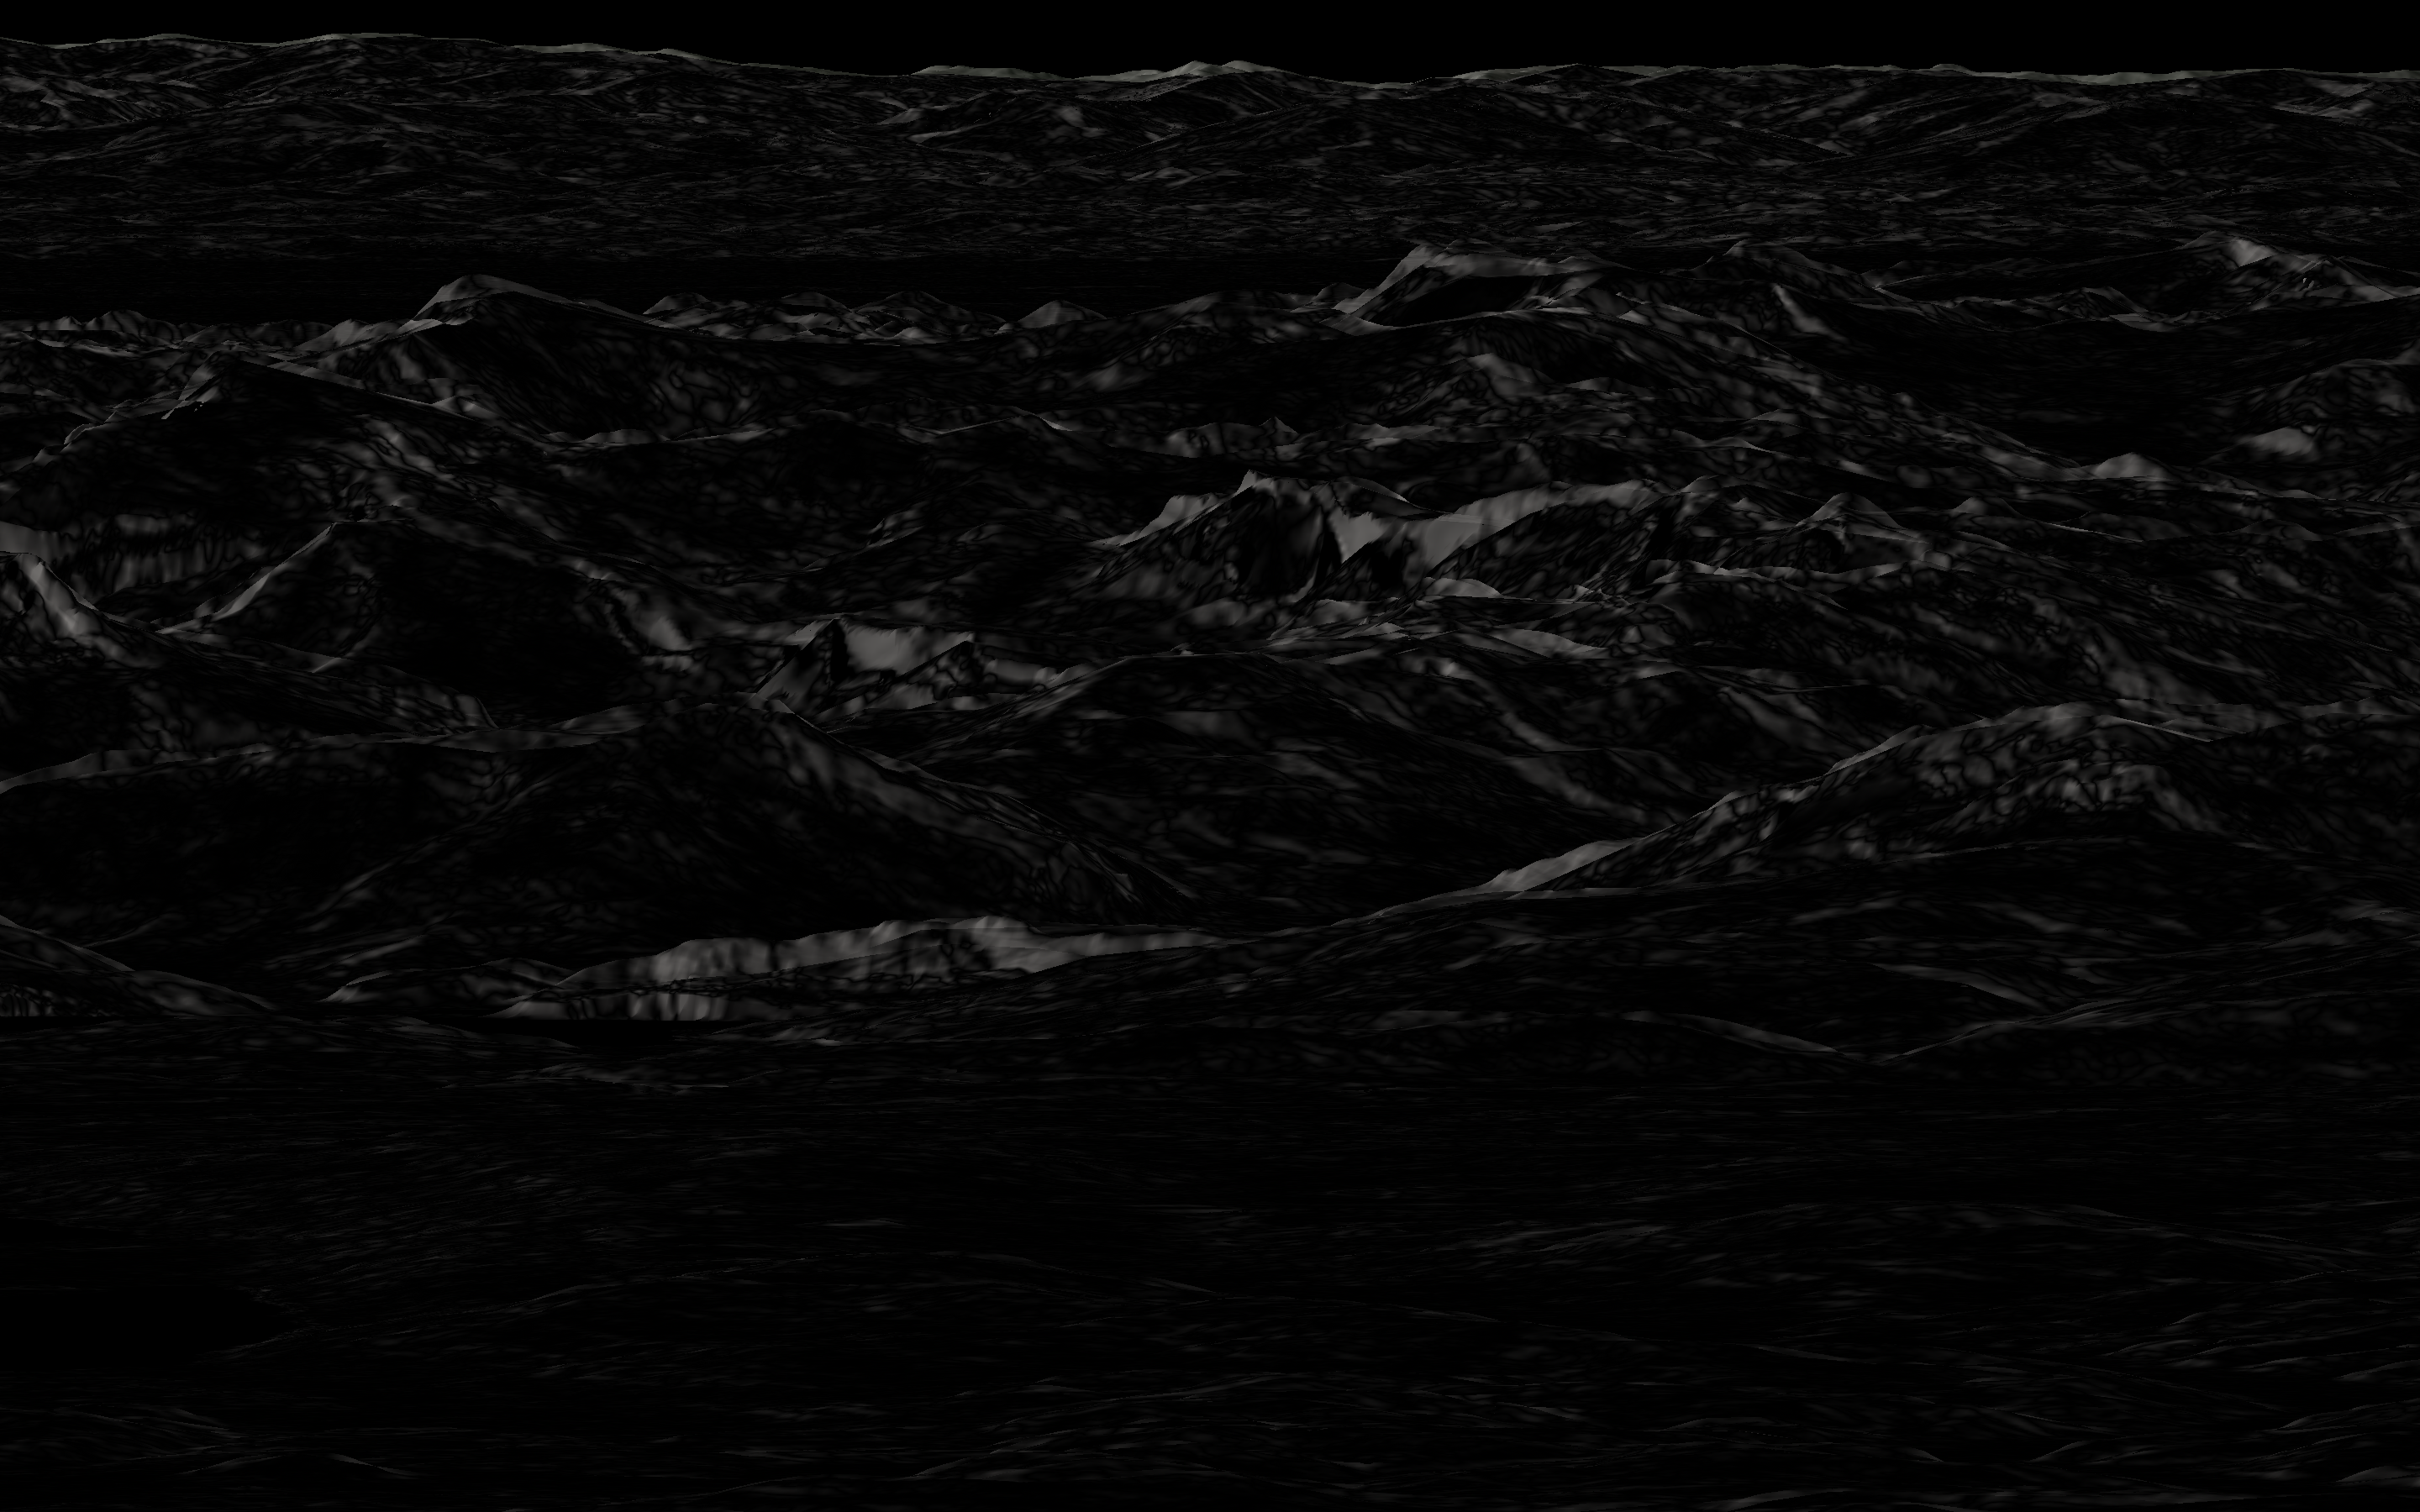
\includegraphics[width=0.4\textwidth]{results-accuracy-zoom-3-diff} }}
  \qquad
  \subfloat[\centering Absolute difference (binarised).]{{\includegraphics[width=0.4\textwidth]{results-accuracy-zoom-3-diff-bin} }}
  \caption{Screenshot showcasing the screenshot of a small section of the terrain with no LOD (a), with LOD (b),
  the absolute difference (c) between (a) and (b) and the binarised absolute difference (d) of (c). The FOV is set to $2^{\circ}$ and the computed RSME is 4.78.}\label{fig:results-zoom-3}
\end{figure}

\subsubsection{Low FOV Screenshot 4}
\begin{figure}[H]
  \centering
  \subfloat[\centering No LOD.]{{\includegraphics[width=0.4\textwidth]{results-accuracy-zoom-4-no-lod} }}
  \qquad
  \subfloat[\centering With LOD.]{{\includegraphics[width=0.4\textwidth]{results-accuracy-zoom-4-lod} }}
  \qquad
  \subfloat[\centering Absolute difference.]{{\includegraphics[width=0.4\textwidth]{results-accuracy-zoom-4-diff} }}
  \qquad
  \subfloat[\centering Absolute difference (binarised).]{{\includegraphics[width=0.4\textwidth]{results-accuracy-zoom-4-diff-bin} }}
  \caption{Screenshot showcasing the screenshot of a small section of the terrain with no LOD (a), with LOD (b),
  the absolute difference (c) between (a) and (b) and the binarised absolute difference (d) of (c). The FOV is set to $1^{\circ}$ and the computed RSME is 5.3.}\label{fig:results-zoom-4}
\end{figure}
\subsubsection{Low FOV Screenshot 5}
\begin{figure}[H]
  \centering
  \subfloat[\centering No LOD.]{{\includegraphics[width=0.4\textwidth]{results-accuracy-zoom-5-no-lod} }}
  \qquad
  \subfloat[\centering With LOD.]{{\includegraphics[width=0.4\textwidth]{results-accuracy-zoom-5-lod} }}
  \qquad
  \subfloat[\centering Absolute difference.]{{\includegraphics[width=0.4\textwidth]{results-accuracy-zoom-5-diff} }}
  \qquad
  \subfloat[\centering Absolute difference (binarised).]{{\includegraphics[width=0.4\textwidth]{results-accuracy-zoom-5-diff-bin} }}
  \caption{Screenshot showcasing the screenshot of a small section of the terrain with no LOD (a), with LOD (b),
  the absolute difference (c) between (a) and (b) and the binarised absolute difference (d) of (c). The FOV is set to $1^{\circ}$ and the computed RSME is 4.49.}\label{fig:results-zoom-5}
\end{figure}

\end{document}
